\documentclass[a4paper]{article}

\addtolength{\oddsidemargin}{-.5in}
\addtolength{\evensidemargin}{-.5in}	\addtolength{\textwidth}{1.375in}

\addtolength{\topmargin}{-.5in}
\addtolength{\textheight}{1.375in}

\usepackage[british]{babel}
\usepackage[UKenglish]{datetime}
\usepackage{textcomp}
\usepackage{gensymb}
\usepackage{pgfplots}
\usepackage{blindtext}
\usepackage{scalerel,amssymb}
\def\msquare{\mathord{\scalerel*{\Box}{gX}}}
% \usepackage{epstopdf}
% \epstopdfDeclaregraphicsRule{.tif}{png}{.png}{convert #1 \OutputFile}
% \AppendGraphicsExtentions{.tif}
\pgfplotsset{compat=1.16}
\usepackage[utf8]{inputenc}
\usepackage{amsmath}
\usepackage{graphicx}
\usepackage{xcolor}
\usepackage{soul}
\usepackage{subcaption}
%\usepackage{circuitikz}
\usepackage[colorinlistoftodos]{todonotes}
\usetikzlibrary{positioning,fit,calc,arrows.meta, positioning}
\tikzset{block/.style={draw,thick,text width=2cm,minimum height=1cm,align=center},
         line/.style={-latex}
         }
\usepackage{listings}
\usepackage{lipsum}
\usepackage{courier}
\usepackage{hyperref}
\usepackage{import}
\usepackage{pdfpages}
\usepackage[nottoc]{tocbibind}

\usepackage{setspace}
\usepackage[acronym, toc]{glossaries}
\usepackage[titletoc, page]{appendix}
\newglossaryentry{latex}
{
    name=latex,
    description={Is a mark up language specially suited for scientific documents}
}

\newglossaryentry{maths}
{
    name=mathematics,
    description={Mathematics is what mathematicians do}
}

\newglossaryentry{formula}
{
    name=formula,
    description={A mathematical expression}
}

\newacronym{gcd}{GCD}{Greatest Common Divisor}

\newacronym{lcm}{LCM}{Least Common Multiple}

\newacronym{tlm}{TLM}{Transmission Line Measurement}

\newacronym{tlms}{TLMs}{Transmission Line Measurements}

\newacronym{sem}{SEM}{Scanning Electron Microscope}

\newacronym{ipa}{IPA}{isopropanol}

\newacronym{lor}{LOR}{lift-off resist}

\newacronym{ebpvd}{EBPVD}{electron-beam physical vapor deposition}

%\onehalfspacing
\singlespacing


\definecolor{codegreen}{rgb}{0,0.6,0}
\definecolor{codegray}{rgb}{0.5,0.5,0.5}
\definecolor{codepurple}{rgb}{0.58,0,0.82}
\definecolor{backcolour}{rgb}{0.92,0.96,1}

\lstdefinestyle{mystyle}{
    backgroundcolor=\color{backcolour},
    commentstyle=\color{codegreen},
    keywordstyle=\color{magenta},
    numbers=left,
    numberstyle=\tiny\color{codegray},
    stringstyle=\color{codepurple},
    basicstyle=\footnotesize\ttfamily,
    breakatwhitespace=false,
    breaklines=true,
    captionpos=b,
    keepspaces=true,
    showspaces=false,
    showstringspaces=false,
    showtabs=false,
    tabsize=2
}

\lstset{style=mystyle}


\title{Manufacture of Red LEDs from a GaAs Substrate}

\author{Angus Bruce}\date{\today}



\begin{document}
  \clearpage
\vfill
  \maketitle
  \begin{center}
    \vfill
    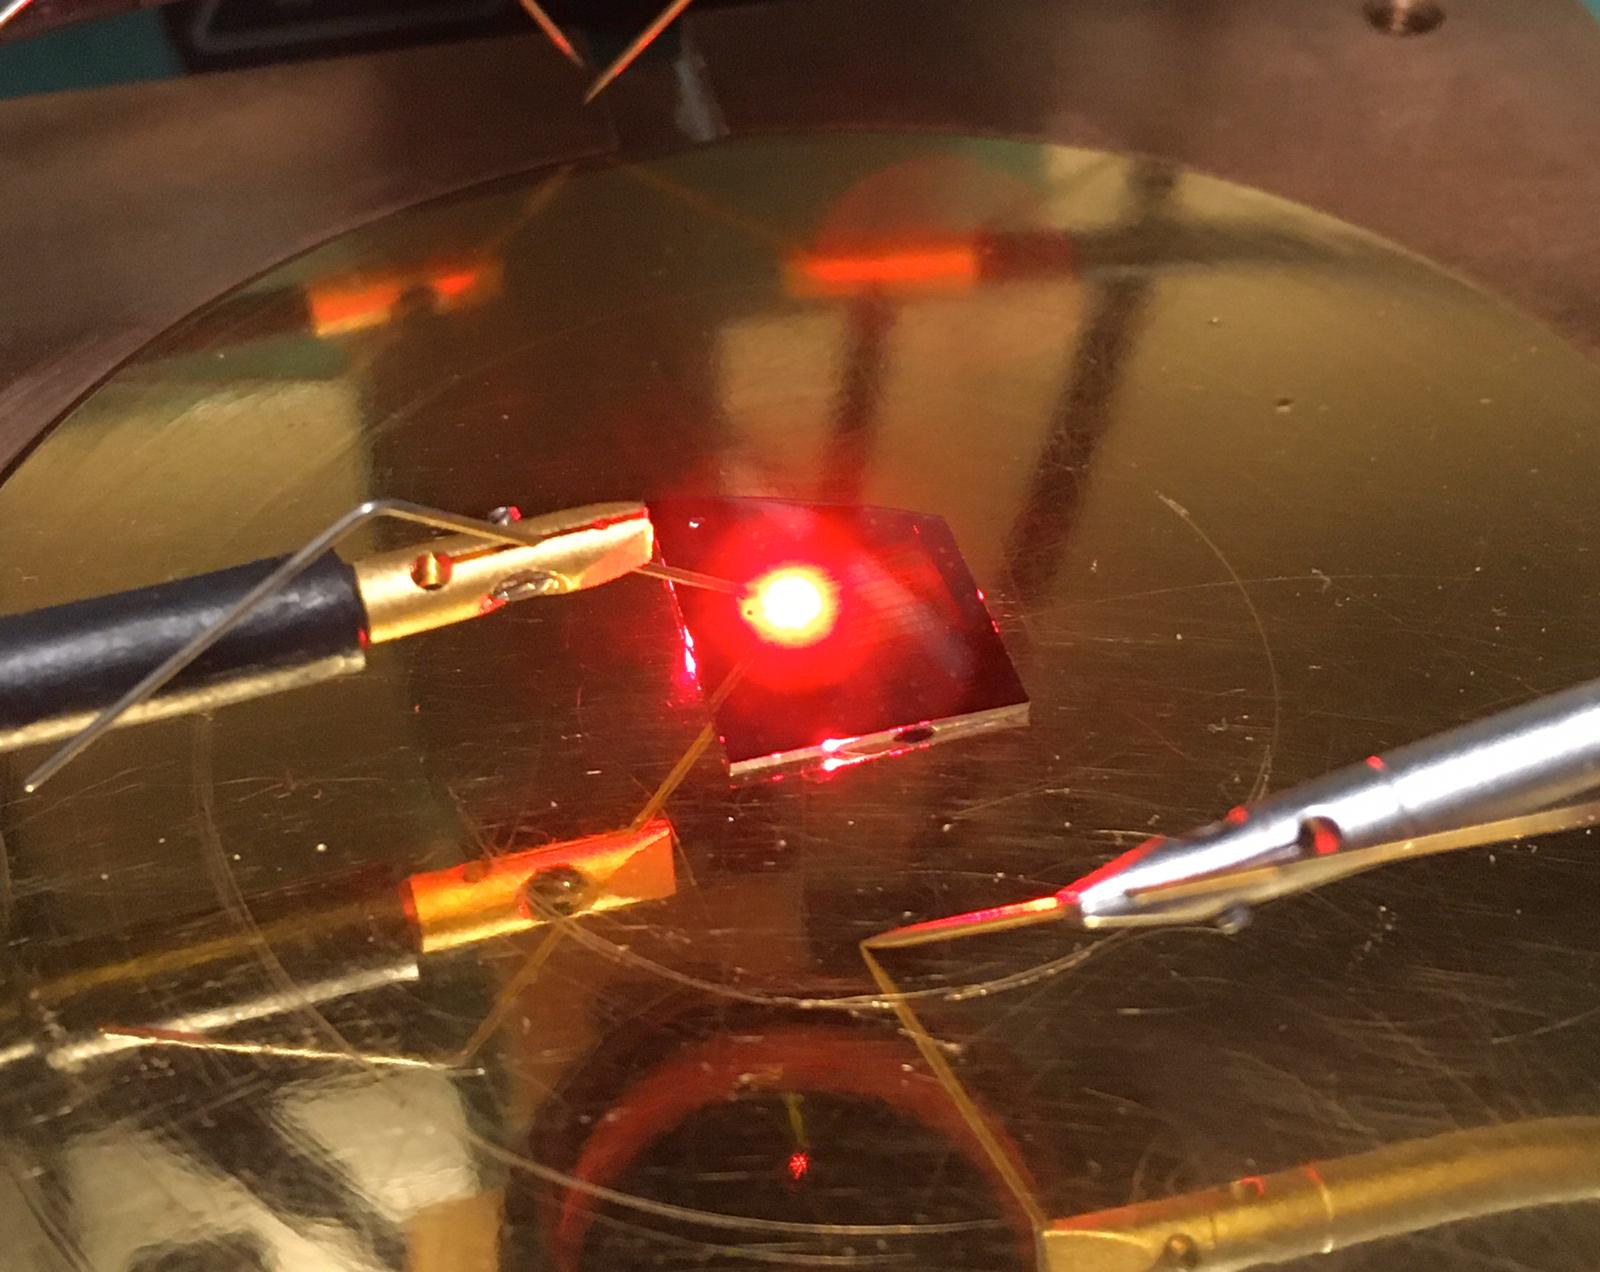
\includegraphics[width=8cm]{Figures/LED_on_picture.jpeg}
    \vfill
    Completed in partial fulfilment of the Degree of Master of Engineering in Electronics with Music

    \vspace{1.5cm}

    James Watt School of Engineering

    University of Glasgow

    \vfill
    
\includegraphics[width=6cm]{Figures/logo-glasgow-university-1-transparent.png}
    \vfill
  \end{center}
  \thispagestyle{empty}

  % \newpage
  % \thispagestyle{empty}
  % \begin{abstract}

  Lorem ipsum dolor sit amet, consectetur adipiscing elit. Sed ullamcorper molestie sem sit amet elementum. Integer id luctus lacus. Vivamus quis fringilla neque. Nam turpis lectus, sollicitudin sed dui sed, gravida aliquam urna. Ut luctus at nunc in luctus. Etiam lobortis felis nec vehicula aliquet. Nam dictum lectus volutpat, bibendum dolor sagittis, pretium tortor. Morbi vitae vulputate turpis, sit amet facilisis mauris. Donec sollicitudin lectus nec lectus ultricies, non lacinia est scelerisque. Suspendisse potenti. Ut fermentum nibh diam, et tincidunt lacus semper vel. Pellentesque ac velit metus.

  Orci varius natoque penatibus et magnis dis parturient montes, nascetur ridiculus mus. Phasellus vitae odio finibus, ultricies felis ac, dignissim neque. Proin lacinia interdum ipsum, eget maximus dui pretium quis. Duis at nulla eget ipsum interdum vehicula nec feugiat erat. Vivamus massa ligula, condimentum faucibus est sed, vulputate imperdiet dui. Nullam lobortis fermentum nulla. Morbi vitae magna libero. Integer aliquet tortor id fringilla vulputate. Sed nec mauris eu nunc blandit tincidunt. Donec vel sapien nec elit aliquet tincidunt sit amet non ligula. Donec ornare mauris ut aliquam tempus.

  Sed sit amet massa in purus imperdiet interdum. Proin iaculis, nibh id vehicula interdum, tellus diam elementum nunc, nec mattis dolor neque ac arcu. Etiam turpis leo, porttitor ac rutrum at, mattis at est. Aliquam varius imperdiet porttitor. Vivamus vestibulum pulvinar nisi et tincidunt. Suspendisse vel ante aliquam, dapibus metus in, molestie velit. Aliquam erat volutpat. Vivamus sit amet congue orci.

\end{abstract}



  % \newpage
  % \thispagestyle{empty}
  % \renewcommand{\abstractname}{Acknowledgements}
\begin{abstract}
  % \begin{center}
    ma Maw 'n' tha'
  % \end{center}
\end{abstract}



  \newpage
  \pagestyle{empty}
  % \thispagestyle{empty}
  \tableofcontents
  % \thispagestyle{empty}
  \listoffigures
  % \thispagestyle{empty}
  \listoftables
  %\newpage
  % \printglossary
  % \printglossary[type=\acronymtype]


  \newpage
  % \pagenumbering{arabic}
  \pagestyle{plain}
  % \onehalfspacing
  \spacing{1.5}

  \newpage
\section{Introduction}
\label{sec:intro}

An LED emit photons due to the recombination of electrons and holes when a potential difference is applied across it. LEDs are almost always made from a direct bandgap semiconductor such as GaAs as the recombination rate is higher due to the probability of a phonon, electron and hole being in close proximity is lower in an indirect bandgap semiconductor such as silicon. The wavelength of light produced by an LED depends largely on its bandgap. Using InGaAsP and altering the ratios, the bandgap can be tailored. Using InGaAsP and other direct bandgap semiconductors, LEDs are able to produce a wide range of wavelengths ranging from infrared through visible to ultraviolet.

The applications of LEDs in the world today are as useful as they are varied. In the home, LEDs provide energy-efficient long-lifetime lighting, far outperforming traditional incandescent bulbs. Due to their high ratio of optical power to area, it is possible to make high-resolution displays and screens from them. They are used in streetlights, reducing their running cost and carbon footprints. Small LEDs can be switched on an off very quickly making them suitable for using in optical communication systems. Since it is possible to engineer LEDs with small wavelengths, LEDs can be useful in wavelength division multiplexing which can vastly increase the bandwidth of a given channel.

This report details the manufacture and testing of a red AlInGaP LED. The p and n contact layers are heavily doped GaAs.


%
% \subsection{subsection1}
\label{sec:intro:subsection1}
\subsubsection{subsubsection1}
\label{sec:intro:subsubsection1}

Hello World!


%
% This is an example of a citation: \cite{lin_koizumi_yater_koeck_2014, emission_suppression_08}
%
%
%
% \begin{table}[ht]
% \centering
%  \begin{tabular}{| c | c | c | c |}
%  \hline
%  Semiconductor & Electron Mobility ($cm^2.V^{-1}.s^{-1}$) & Hole Mobility ($cm^2.V^{-1}.s^{-1}$) & Band Gap (eV) \\ %[0.5ex]
%  \hline\hline
%  Diamond & 4500 & 3800 & 5.47\\
%  Silicon & 1450 & 480 & 1.12\\
%  GaAs & 8500 & 400 & 1.43\\
%  GaN & 1100 & 200 & 3.45\\
%  \hline
% \end{tabular}
% \caption{Example table}
% \label{tab:example}
% \end{table}
%
%
%
%
% \begin{figure}[!htb]
%   \centering
%   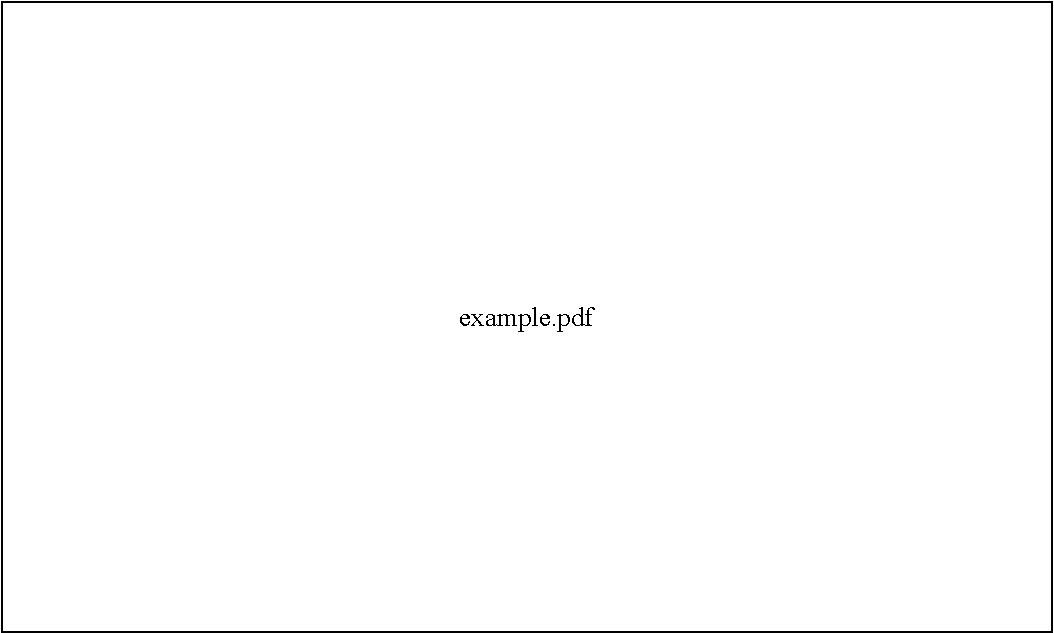
\includegraphics[width=0.67\textwidth]{Figures/example.pdf}
%   \caption{Example Figure}
%   \label{fig:example}
% \end{figure}
%
% Here's an example equation:
%
% \begin{center}
% \begin{equation}
% \%_{err}(V) = \left(\frac{R(V)}{R_{avg}}-1\right)\times100
% \end{equation}
% \end{center}
%
% Here's an example plot with subplots:
%
% \begin{figure*}[!htb]
  \centering
  \begin{subfigure}[t]{0.5\textwidth}
      % \begin{figure}[!htb]
\begin{center}
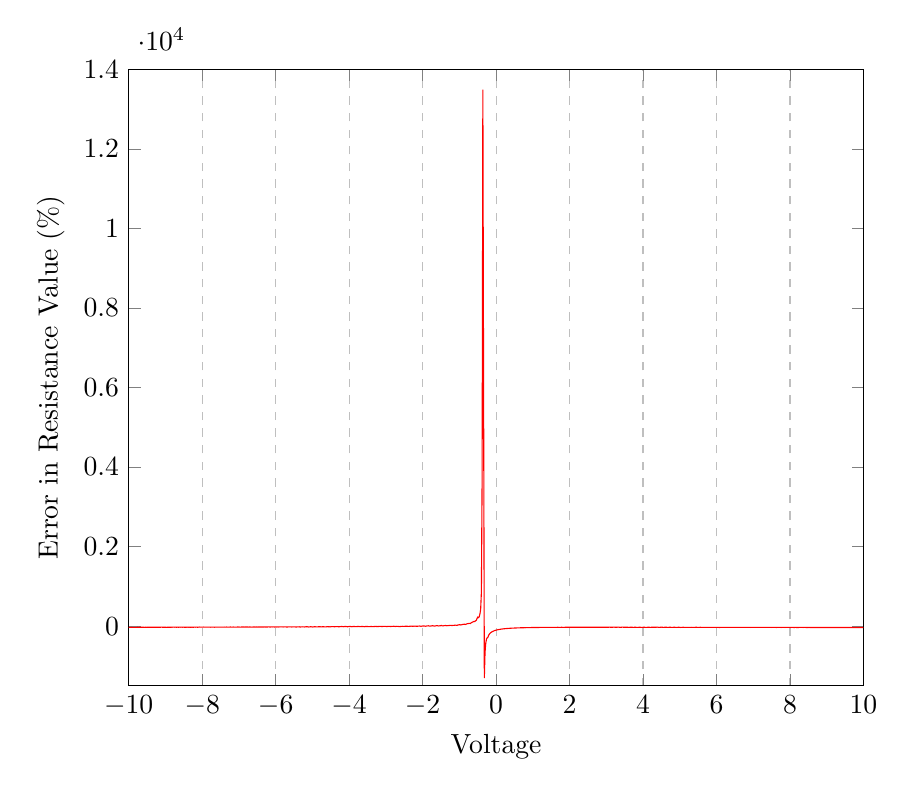
\begin{tikzpicture}

\begin{axis}[
    %title={Temperature dependence of CuSO$_4\cdot$5H$_2$O solubility},
    xlabel={Voltage},
    ylabel={Error in Resistance Value (\%)},
    % height=8cm,
    width=0.9\textwidth,
    xmin=-10, xmax=10,
    ymin=-1500, ymax=14000,
    xtick={-10, -8, -6, -4, -2, 0, 2, 4, 6, 8, 10},
    ytick={-2000, 0, 2000, 4000, 6000, 8000, 10000, 12000, 14000},
    legend pos=south east,
    xmajorgrids=true,
    grid style=dashed,
]

\addplot[color=red]
  coordinates {
  (-10.0,-30.364475134465007)
(-9.98,-28.849073474295984)
(-9.96,-28.423593785412805)
(-9.94,-30.78228828365822)
(-9.92,-28.13613833876788)
(-9.9,-28.85477695538019)
(-9.88,-28.998504678702663)
(-9.86,-28.570798792364048)
(-9.84,-29.847182664035323)
(-9.82,-28.860572428094823)
(-9.8,-29.005459245960196)
(-9.78,-29.150346063825594)
(-9.76,-27.542222126691584)
(-9.74,-29.440119699556366)
(-9.72,-28.43066236196965)
(-9.7,-27.38755644646339)
(-9.68,-29.30465641456027)
(-9.66,-26.461344952595102)
(-9.64,-27.836705581846076)
(-9.62,-28.581575497825117)
(-9.6,-26.293475219249117)
(-9.58,-28.878533603863264)
(-9.56,-28.43557109568967)
(-9.54,-26.75414099912882)
(-9.52,-29.323970762920492)
(-9.5,-26.43246920455763)
(-9.48,-27.214806779008494)
(-9.46,-29.18415298799418)
(-9.44,-25.614599333110622)
(-9.42,-27.675472558888192)
(-9.4,-27.829027818848083)
(-9.38,-26.730106262787256)
(-9.36,-28.136138338767893)
(-9.34,-25.751275673019023)
(-9.32,-25.91026651740229)
(-9.3,-27.981259326566942)
(-9.28,-25.569571850866733)
(-9.26,-26.387239050552058)
(-9.24,-27.190561211646404)
(-9.22,-26.050803067348195)
(-9.2,-27.505753587353578)
(-9.18,-26.371623878335836)
(-9.16,-25.870160718819125)
(-9.14,-27.978542150914286)
(-9.12,-24.14370157981056)
(-9.1,-25.004456293897682)
(-9.08,-27.17367590580495)
(-9.06,-26.679438440229397)
(-9.04,-28.136138338767893)
(-9.02,-28.295129183151147)
(-9.0,-27.165005073075555)
(-8.98,-29.239311653742938)
(-8.96,-28.136138338767868)
(-8.94,-27.650571705921724)
(-8.92,-28.456959149755523)
(-8.9,-25.973568427665995)
(-8.88,-26.81753537250674)
(-8.86,-26.98236074328939)
(-8.84,-25.08531402296087)
(-8.82,-26.63897455415889)
(-8.8,-24.714049688233008)
(-8.78,-24.162895987305532)
(-8.76,-26.457076150421344)
(-8.74,-23.775467121460103)
(-8.72,-24.68114498967019)
(-8.7,-28.30096370955053)
(-8.68,-23.556578527022698)
(-8.66,-25.91178071592022)
(-8.64,-26.082885148446955)
(-8.62,-24.084989274531765)
(-8.6,-26.425094013500463)
(-8.58,-23.689117196364894)
(-8.56,-24.61340002204082)
(-8.54,-26.93840731108069)
(-8.52,-24.22275973345327)
(-8.5,-25.86858930576784)
(-8.48,-26.04301615446015)
(-8.46,-26.217443003152454)
(-8.44,-27.793929473714396)
(-8.42,-24.363285601553198)
(-8.4,-25.290044807629975)
(-8.38,-26.915150397921693)
(-8.36,-23.60352448017542)
(-8.34,-26.550906096240713)
(-8.32,-27.438430943998636)
(-8.3,-24.611975254268625)
(-8.28,-27.07931684374978)
(-8.26,-24.517357919407768)
(-8.24,-27.43159067542247)
(-8.22,-23.797607990798753)
(-8.2,-24.682558074884554)
(-8.18,-26.149951207427304)
(-8.16,-23.003005362965588)
(-8.14,-25.613958046486584)
(-8.12,-26.912004422694803)
(-8.1,-24.754746709413123)
(-8.08,-21.7860988385297)
(-8.06,-23.5450468598824)
(-8.04,-24.214920283800346)
(-8.02,-25.11068470334179)
(-8.0,-25.219706908187177)
(-7.98,-23.250319050236566)
(-7.96,-22.023399833232325)
(-7.94,-22.472953588290345)
(-7.92,-23.82738432053554)
(-7.9,-24.8246150524717)
(-7.88,-25.09428176051468)
(-7.86,-23.086880084792426)
(-7.84,-22.352167113552944)
(-7.82,-23.143408343704163)
(-7.8,-23.757056452990955)
(-7.78,-25.888011171210778)
(-7.76,-25.525698919449624)
(-7.74,-24.752937059261825)
(-7.72,-24.374453104592163)
(-7.7,-23.99014631985065)
(-7.68,-24.436684343063707)
(-7.66,-26.249038005755885)
(-7.64,-24.416312900356086)
(-7.62,-23.433637324022826)
(-7.6,-22.595613856949537)
(-7.58,-23.920660420092265)
(-7.56,-25.454062272377232)
(-7.54,-25.240960689060397)
(-7.52,-23.23632958913843)
(-7.5,-22.64940263214109)
(-7.48,-23.20833068199769)
(-7.46,-23.23820045922228)
(-7.44,-23.879964299606073)
(-7.42,-24.770054525064577)
(-7.4,-23.32863663594035)
(-7.38,-22.18965682806734)
(-7.36,-22.85326402761546)
(-7.34,-21.9703040542243)
(-7.32,-23.717594640339456)
(-7.3,-24.71208522861733)
(-7.28,-23.063395162680912)
(-7.26,-22.63765782020386)
(-7.24,-21.924616082334868)
(-7.22,-22.046712560983185)
(-7.2,-23.63934416161878)
(-7.18,-23.125368485153963)
(-7.16,-21.754067899266726)
(-7.14,-22.350488459261907)
(-7.12,-22.474137116973825)
(-7.1,-22.69190639473515)
(-7.08,-23.558272151213423)
(-7.06,-22.94063436690481)
(-7.04,-21.925681158167563)
(-7.02,-22.33923816781873)
(-7.0,-21.10303769940012)
(-6.98,-22.686536005641145)
(-6.96,-23.66109933422228)
(-6.94,-21.975093878449492)
(-6.92,-20.508644070376235)
(-6.9,-22.13243632812474)
(-6.88,-20.56179816367657)
(-6.86,-22.094486252204113)
(-6.84,-22.321616029894486)
(-6.82,-21.254573179691015)
(-6.8,-20.669763101237272)
(-6.78,-21.514661394466216)
(-6.76,-20.517064000338813)
(-6.74,-22.576338299759513)
(-6.72,-22.209221913099253)
(-6.7,-20.911978789379905)
(-6.68,-22.17078536040361)
(-6.66,-22.80430344132163)
(-6.64,-21.825681285946718)
(-6.62,-22.86985016255566)
(-6.6,-21.159992193462106)
(-6.58,-20.016202684217298)
(-6.56,-23.27035603878863)
(-6.54,-20.9304079299364)
(-6.52,-19.54801201386789)
(-6.5,-22.663062781786625)
(-6.48,-21.655817031496603)
(-6.46,-20.06877645806483)
(-6.44,-20.969387107524796)
(-6.42,-20.123616366843798)
(-6.4,-19.928844945702373)
(-6.38,-22.025265748527055)
(-6.36,-20.760374451207298)
(-6.34,-20.123267368125596)
(-6.32,-21.585012828213568)
(-6.3,-19.153155631113872)
(-6.28,-19.753724887528858)
(-6.26,-20.797927112796998)
(-6.24,-19.693678945901073)
(-6.22,-19.721045342517286)
(-6.2,-18.93086930501471)
(-6.18,-17.877465779139346)
(-6.16,-20.609507203516884)
(-6.14,-21.876042740799374)
(-6.12,-19.034088113633917)
(-6.1,-18.336520839508964)
(-6.08,-19.799508278213796)
(-6.06,-18.38549444020491)
(-6.04,-20.560445747832723)
(-6.02,-20.23959306773281)
(-6.0,-19.314526577957956)
(-5.98,-19.462913655515724)
(-5.96,-19.732268459343437)
(-5.94,-18.660187067888945)
(-5.92,-19.91075658236181)
(-5.9,-19.207929915916633)
(-5.88,-17.59760012323618)
(-5.86,-18.51350051570816)
(-5.84,-18.539411470963596)
(-5.82,-18.692131635231167)
(-5.8,-19.844154300933415)
(-5.78,-19.25094859993748)
(-5.76,-17.608311471198856)
(-5.74,-19.433873840728054)
(-5.72,-19.082423483809507)
(-5.7,-21.588052934719936)
(-5.68,-21.74334082902637)
(-5.66,-18.519740183779287)
(-5.64,-16.807844874928346)
(-5.62,-18.17769397566359)
(-5.6,-16.851730309318224)
(-5.58,-18.09633413609575)
(-5.56,-20.595574158098074)
(-5.54,-17.469777445434097)
(-5.52,-16.521776858164717)
(-5.5,-16.402022179192755)
(-5.48,-16.706014825813863)
(-5.46,-19.857703294459284)
(-5.44,-23.16442463893421)
(-5.42,-17.895841019418622)
(-5.4,-16.938173593610127)
(-5.38,-17.103864550294002)
(-5.36,-15.823798403801536)
(-5.34,-21.23295950924067)
(-5.32,-20.483414301631676)
(-5.3,-16.327226097423065)
(-5.28,-15.90399167302624)
(-5.26,-16.95871873065006)
(-5.24,-17.564221737115528)
(-5.22,-19.9809390205564)
(-5.2,-18.62106257874411)
(-5.18,-14.776830722256785)
(-5.16,-15.569780015492318)
(-5.14,-14.17745145475533)
(-5.12,-17.575499169912977)
(-5.1,-21.147656094603327)
(-5.08,-17.777383504716404)
(-5.06,-15.669958254676597)
(-5.04,-15.69044162648746)
(-5.02,-16.025003366064904)
(-5.0,-19.651317462844233)
(-4.98,-19.54091028036511)
(-4.96,-16.091159642252517)
(-4.94,-14.661664277286857)
(-4.92,-15.816619196842375)
(-4.9,-16.158828061895857)
(-4.88,-18.518669863658754)
(-4.86,-19.003161485717047)
(-4.84,-15.248272309852961)
(-4.82,-13.576892912390514)
(-4.8,-15.784537115743614)
(-4.78,-15.641144710046762)
(-4.76,-16.972820022459977)
(-4.74,-16.017084745009804)
(-4.72,-13.821791910311088)
(-4.7,-12.948414997992009)
(-4.68,-17.080159621655255)
(-4.66,-16.61215255444678)
(-4.64,-16.804311849272203)
(-4.62,-16.327862682738814)
(-4.6,-13.189662909225907)
(-4.58,-13.018898940686285)
(-4.56,-16.06065338749527)
(-4.54,-14.68045712813969)
(-4.52,-17.1365676763344)
(-4.5,-14.53821948320705)
(-4.48,-11.357351254867854)
(-4.46,-12.523792846862658)
(-4.44,-12.53411574126353)
(-4.42,-12.544529586275887)
(-4.4,-14.632561741516914)
(-4.38,-12.759502750499818)
(-4.36,-10.784044179108188)
(-4.34,-11.193291682873753)
(-4.32,-9.541992314533)
(-4.3,-12.410826206548165)
(-4.28,-15.686039498335113)
(-4.26,-12.830281697935986)
(-4.24,-10.170172923459852)
(-4.22,-9.52699993723164)
(-4.2,-7.979201531349123)
(-4.18,-10.597934004776732)
(-4.16,-13.895833954284099)
(-4.14,-10.602047092097067)
(-4.12,-8.842638533166147)
(-4.1,-9.061162712638371)
(-4.08,-8.602071203919259)
(-4.06,-12.539784668884192)
(-4.04,-14.809271974360982)
(-4.02,-9.946158392096926)
(-4.0,-9.033086504769472)
(-3.98,-8.32750980394108)
(-3.96,-8.553697886092792)
(-3.94,-12.609995387267114)
(-3.92,-13.692911240186923)
(-3.9,-9.473817674804508)
(-3.88,-9.470200244941351)
(-3.86,-7.781081777807197)
(-3.84,-10.63561244199116)
(-3.82,-12.684493783108564)
(-3.8,-12.697354759372747)
(-3.78,-8.227906392075202)
(-3.76,-7.967261632754507)
(-3.74,-6.155432048530674)
(-3.72,-10.4110035590538)
(-3.7,-12.76368499128646)
(-3.68,-9.6792995514569)
(-3.66,-6.331291424462404)
(-3.64,-7.632607186834428)
(-3.62,-8.656187073855248)
(-3.6,-10.912568188555227)
(-3.58,-13.317848804848042)
(-3.56,-9.406746631024676)
(-3.54,-7.826786130158803)
(-3.52,-8.081107177493807)
(-3.5,-8.868291371625936)
(-3.48,-10.683486221040084)
(-3.46,-12.447548821174959)
(-3.44,-11.202699671466053)
(-3.42,-9.375218701543576)
(-3.4,-8.829429235750297)
(-3.38,-9.635471571813792)
(-3.36,-10.436730273835348)
(-3.34,-11.233247800105294)
(-3.32,-8.235376647965154)
(-3.3,-7.072592679441225)
(-3.28,-6.462910218713757)
(-3.26,-7.327456876733896)
(-3.24,-7.603606435558696)
(-3.22,-10.724678028870594)
(-3.2,-7.570595934106594)
(-3.18,-6.647434606732794)
(-3.16,-6.316087933377268)
(-3.14,-6.290479395237192)
(-3.12,-9.0035517925957)
(-3.1,-9.586862358027782)
(-3.08,-7.15574919605918)
(-3.06,-6.503649369315356)
(-3.04,-5.507725151321097)
(-3.02,-4.476733179172099)
(-3.0,-7.072592679441225)
(-2.98,-11.065486814588166)
(-2.96,-6.703056790681106)
(-2.94,-7.007150843299992)
(-2.92,-5.646368682195247)
(-2.9,-5.61358749204115)
(-2.88,-8.258900006937731)
(-2.86,-9.537568507427896)
(-2.84,-4.8071981726216295)
(-2.82,-4.766875054194286)
(-2.8,-3.6308368527538604)
(-2.78,-2.8299925008631988)
(-2.76,-6.793111755168879)
(-2.74,-7.119348607652832)
(-2.72,-3.424059427593207)
(-2.7,-5.626251709471431)
(-2.68,-5.218922612154476)
(-2.66,-5.926244085198107)
(-2.64,-11.179496823196256)
(-2.62,-8.777462426149151)
(-2.6,-8.048208504328969)
(-2.58,-3.833629104782754)
(-2.56,-4.181517785023836)
(-2.54,-3.318745434571202)
(-2.52,-6.45819659798299)
(-2.5,-5.242798442468189)
(-2.48,-3.140012543556703)
(-2.46,-0.9052131801395746)
(-2.44,-1.2681179879468818)
(-2.42,-2.077395709357144)
(-2.4,-5.442287287852476)
(-2.38,-4.127807873468359)
(-2.36,-3.1970813239110885)
(-2.34,-2.2317230887888617)
(-2.32,1.1675722415403378)
(-2.3,-0.6689412134411765)
(-2.28,-3.844128763140131)
(-2.26,-1.9249230951784102)
(-2.24,0.10886201564672682)
(-2.22,-0.7849671094929733)
(-2.2,1.3464715735324706)
(-2.18,-2.085488486571241)
(-2.16,-3.4664544849120738)
(-2.14,-1.9204949266347304)
(-2.12,0.23117547487636614)
(-2.1,1.9689928976942328)
(-2.08,3.803355732890834)
(-2.06,-0.5110517324340313)
(-2.04,-2.525081257371342)
(-2.02,0.8090281636728314)
(-2.0,3.8495110711446845)
(-1.98,4.013483983362254)
(-1.96,6.064133174710062)
(-1.94,-0.41722026943550317)
(-1.92,-0.8774321914039818)
(-1.9,2.201599667919929)
(-1.88,5.550046814934673)
(-1.86,8.495765170366653)
(-1.84,10.191254547222584)
(-1.82,3.474864100824737)
(-1.8,1.0585554611076686)
(-1.78,3.829280646910038)
(-1.76,6.107715204503794)
(-1.74,11.645642223699904)
(-1.72,10.36235897974931)
(-1.7,6.790703517565189)
(-1.68,1.2846372406627227)
(-1.66,5.0123330613074835)
(-1.64,8.324203239357232)
(-1.62,13.690874893746141)
(-1.6,14.069621684495438)
(-1.58,6.715132917995059)
(-1.56,5.364308450678679)
(-1.54,8.927506848717993)
(-1.52,10.113981577694364)
(-1.5,16.159259150698468)
(-1.48,15.607081802851663)
(-1.46,6.627274416055773)
(-1.44,7.795792491848186)
(-1.42,12.883499512112383)
(-1.4,14.328870824687456)
(-1.38,16.94826543926924)
(-1.36,14.176228807565039)
(-1.34,11.455526187559073)
(-1.32,15.121720136925255)
(-1.3,15.622549702477407)
(-1.28,12.727626135266057)
(-1.26,19.773102768720218)
(-1.24,21.603696042477914)
(-1.22,20.829535869216052)
(-1.2,13.82871435253239)
(-1.18,18.966549888122742)
(-1.16,18.412044782712012)
(-1.14,21.7669475234908)
(-1.12,25.604751967197203)
(-1.1,25.07950605594198)
(-1.08,21.57420205847538)
(-1.06,20.22678876405626)
(-1.04,28.504842035215617)
(-1.02,32.217061497937884)
(-1.0,37.14477416265672)
(-0.98,36.69756294256108)
(-0.96,30.661566656785656)
(-0.94,35.32057283965984)
(-0.92,41.99903936497758)
(-0.9,43.60007880796826)
(-0.88,46.66094216577983)
(-0.86,51.47774761926376)
(-0.84,43.182267066971015)
(-0.82,46.15170278325975)
(-0.8,57.59618785357921)
(-0.78,62.19274333264193)
(-0.76,63.326958320982094)
(-0.74,67.86381827434269)
(-0.72,70.65296964408682)
(-0.7,67.68234387620826)
(-0.68,82.88707308996199)
(-0.66,93.11949794956513)
(-0.64,104.59462394656826)
(-0.62,110.96398783126853)
(-0.6,119.09713921107357)
(-0.58,115.29462687765819)
(-0.56,136.17231531860324)
(-0.54,142.5405331066584)
(-0.52,190.13360298012964)
(-0.5,227.84608422094945)
(-0.48,214.73224085211146)
(-0.46,235.9489467903128)
(-0.44,304.970531902435)
(-0.42,424.7361247864653)
(-0.4,845.5771271214754)
(-0.38,3735.4308189983435)
(-0.36,13487.70493594725)
(-0.34,5996.2357696654)
(-0.32,-1302.7424545812908)
(-0.3,-645.5252656470049)
(-0.28,-422.4660459157851)
(-0.26,-320.33731169717396)
(-0.24,-290.7890132599083)
(-0.22,-274.8899288215826)
(-0.2,-223.0545576390961)
(-0.18,-196.82256810645043)
(-0.16,-175.25011692275615)
(-0.14,-157.95472714615494)
(-0.12,-146.66484523456631)
(-0.1,-137.58570170566534)
(-0.08,-126.8148737541911)
(-0.06,-118.64979108855505)
(-0.04,-111.47985010562813)
(-0.02,-105.51103233598407)
(0.0,-100.0)
(0.02,-95.05069823269751)
(0.04,-90.83369111463875)
(0.06,-86.7572736496501)
(0.08,-83.24851709528389)
(0.1,-79.94869931327229)
(0.12,-76.96671100601536)
(0.14,-74.01616572166193)
(0.16,-71.65133662278812)
(0.18,-69.14242581340224)
(0.2,-67.09530143716478)
(0.22,-64.89775851360776)
(0.24,-63.272302387785984)
(0.26,-61.52264408583123)
(0.28,-59.82052463030152)
(0.3,-58.088727647026374)
(0.32,-56.77361704587541)
(0.34,-55.282370122952194)
(0.36,-54.12945000346887)
(0.38,-53.11080454795981)
(0.4,-52.026794618670145)
(0.42,-50.61711076944129)
(0.44,-49.326764213233766)
(0.46,-48.21839541953826)
(0.48,-47.608363308943765)
(0.5,-47.03430007279472)
(0.52,-46.49311560160265)
(0.54,-45.312168408870704)
(0.56,-44.59834453429241)
(0.58,-43.244771563841745)
(0.6,-42.72274575353444)
(0.62,-42.760027967672265)
(0.64,-41.98679179718901)
(0.66,-40.71231412948351)
(0.68,-40.11344861563989)
(0.7,-39.537616390790284)
(0.72,-39.5537612195244)
(0.74,-39.569025421236624)
(0.76,-39.044045912347755)
(0.78,-37.43994185740954)
(0.8,-38.577896016040924)
(0.82,-37.57588287901448)
(0.84,-36.590710298912846)
(0.86,-35.621957261812895)
(0.88,-35.731505831418445)
(0.9,-35.835837802471325)
(0.92,-35.9353171237078)
(0.94,-35.54195614355136)
(0.96,-34.170508401924785)
(0.98,-34.30355930223183)
(1.0,-33.45938735071101)
(1.02,-34.0817096272871)
(1.04,-34.209140732674825)
(1.06,-33.41285545375345)
(1.08,-32.627629692594894)
(1.1,-32.31999329849714)
(1.12,-32.02067140153718)
(1.14,-32.18145505479752)
(1.16,-32.33597440987885)
(1.18,-32.05179746774528)
(1.2,-31.340259559332374)
(1.22,-31.504756854138137)
(1.24,-31.241366929068036)
(1.26,-31.815914387686394)
(1.28,-31.963207894691482)
(1.3,-31.306602823822228)
(1.32,-30.65767734442515)
(1.34,-30.82070788358402)
(1.36,-30.97821196378836)
(1.38,-31.130465907985894)
(1.4,-30.90013301804605)
(1.42,-30.295981175580877)
(1.44,-29.31423443157498)
(1.46,-29.865482603342997)
(1.48,-29.65706662789448)
(1.5,-30.18407222030559)
(1.52,-29.978801458286654)
(1.54,-29.777698630521922)
(1.56,-28.86572069065856)
(1.58,-29.73706595003295)
(1.6,-29.545233665458703)
(1.62,-29.357126279614054)
(1.64,-29.51152325094458)
(1.66,-28.651907680834153)
(1.68,-28.136138338767893)
(1.7,-29.300599060130438)
(1.72,-30.08719340649365)
(1.74,-29.274253794941252)
(1.76,-28.783560515896113)
(1.78,-28.29726807343431)
(1.8,-28.45412002753439)
(1.82,-29.224984727574434)
(1.84,-29.66515667198558)
(1.86,-28.59680411864758)
(1.88,-28.440646227162947)
(1.9,-27.679376506175313)
(1.92,-27.226469203815583)
(1.94,-27.38755644646338)
(1.96,-27.54466622632976)
(1.98,-28.569053168052417)
(2.0,-27.847528452578196)
(2.02,-27.126003737103964)
(2.04,-26.698861105543237)
(2.06,-27.71506102434659)
(2.08,-26.727043012077058)
(2.1,-27.72312763956539)
(2.12,-27.58964509419577)
(2.14,-26.346425308890442)
(2.16,-26.78021642063142)
(2.18,-26.102255461563207)
(2.2,-26.25909717597449)
(2.22,-28.2653898885183)
(2.24,-26.829522672200024)
(2.26,-27.494496716792604)
(2.28,-26.59067894820376)
(2.3,-25.94673753546871)
(2.32,-26.35858699025685)
(2.34,-27.7657060621636)
(2.36,-27.14831893448979)
(2.38,-26.277590192356705)
(2.4,-26.669528917110085)
(2.42,-26.558046782017865)
(2.44,-26.93840731108068)
(2.46,-27.068853264591176)
(2.48,-26.71777264808567)
(2.5,-26.36899419955726)
(2.52,-26.50286875555806)
(2.54,-28.697574757996257)
(2.56,-27.68416436605574)
(2.58,-28.024548491467826)
(2.6,-26.78446695955975)
(2.62,-26.451829081082757)
(2.64,-27.47683685563731)
(2.66,-28.45888023245604)
(2.68,-27.920977076309107)
(2.7,-27.815317527780238)
(2.72,-27.280616176134163)
(2.74,-26.307267607868255)
(2.76,-26.64783351146427)
(2.78,-28.85272955191408)
(2.8,-27.723127639565405)
(2.82,-27.829027818848097)
(2.84,-27.3171769523151)
(2.86,-26.8053260857821)
(2.88,-27.935960451132136)
(2.9,-27.232821641908835)
(2.92,-27.540581474172043)
(2.94,-27.643920108211496)
(2.96,-26.951569190505808)
(2.98,-26.255403667192933)
(3.0,-27.361325814118477)
(3.02,-26.877067986212598)
(3.04,-27.755906266486228)
(3.06,-26.893810943028495)
(3.08,-25.2227385416909)
(3.1,-24.940036674589095)
(3.12,-27.013265500311135)
(3.14,-26.35361435500364)
(3.16,-26.839625370652865)
(3.18,-25.99511655352392)
(3.2,-23.7518709164646)
(3.22,-24.67394708685956)
(3.24,-27.41929183840647)
(3.26,-27.513555378831477)
(3.28,-27.606429284753897)
(3.3,-25.704654297598374)
(3.32,-23.725057316083564)
(3.34,-24.992094391088994)
(3.36,-28.476725360859035)
(3.38,-28.726569127064383)
(3.4,-28.13613833876788)
(3.42,-26.326616642262046)
(3.44,-24.630584111390718)
(3.46,-25.997332932183603)
(3.48,-27.970553404064592)
(3.5,-28.21817471052729)
(3.52,-27.47683685563731)
(3.54,-26.218657111148)
(3.56,-25.97356842766598)
(3.58,-27.07692042312614)
(3.6,-29.39140229791605)
(3.62,-29.3078317354184)
(3.64,-28.13613833876788)
(3.66,-26.775686614668825)
(3.68,-25.88032205343772)
(3.7,-27.430052361747048)
(3.72,-28.90064750537673)
(3.74,-29.419421582718453)
(3.76,-28.13613833876788)
(3.78,-27.289775942329385)
(3.8,-26.59067894820376)
(3.82,-29.393016577698905)
(3.84,-30.172765997183358)
(3.86,-29.950882320112125)
(3.88,-28.284006366877424)
(3.9,-27.165005073075555)
(3.92,-26.79149227857851)
(3.94,-29.636278592133568)
(3.96,-30.92696791784485)
(3.98,-31.640016871007692)
(4.0,-28.422448544589518)
(4.02,-27.047291949961338)
(4.04,-26.9793759780237)
(4.06,-31.05688129853441)
(4.08,-31.10795216686394)
(4.1,-30.90013301804605)
(4.12,-27.996325378337474)
(4.14,-27.07931684374978)
(4.16,-26.583088283220626)
(4.18,-28.614319927768474)
(4.2,-29.479388089445113)
(4.22,-28.6098172762713)
(4.24,-27.31326969379194)
(4.26,-26.408641664219047)
(4.28,-25.92068210258346)
(4.3,-26.98142600583693)
(4.32,-27.19233527755096)
(4.34,-28.46578908033317)
(4.36,-26.380066531256563)
(4.38,-24.76966680779239)
(4.4,-25.564738392320773)
(4.42,-28.588518762894346)
(4.44,-29.408065093833923)
(4.46,-28.584486851805877)
(4.48,-26.293475219249107)
(4.5,-25.55539192551921)
(4.52,-26.443692321383793)
(4.54,-28.825931077226485)
(4.56,-29.617867445185052)
(4.58,-28.572811109278838)
(4.6,-26.211213472842022)
(4.62,-25.624766829101166)
(4.64,-26.875368835939252)
(4.66,-30.694206262139556)
(4.68,-31.41866383063493)
(4.7,-28.802666566654512)
(4.72,-26.51702187153041)
(4.74,-25.690509538778304)
(4.76,-29.323970762920492)
(4.78,-30.519971937562794)
(4.8,-31.449416539365238)
(4.82,-29.01971040837319)
(4.84,-27.657843086446864)
(4.86,-27.479574818607123)
(4.88,-29.066414865126877)
(4.9,-30.791485428451782)
(4.92,-32.11017677164708)
(4.94,-29.337683796479563)
(4.96,-27.903569207178126)
(4.98,-27.49553665459158)
(5.0,-30.579731780108077)
(5.02,-32.188611740717064)
(5.04,-30.879033822021018)
(5.06,-29.199544391387366)
(5.08,-28.474056183569907)
(5.1,-27.625257805631176)
(5.12,-30.733627314475076)
(5.14,-31.596250196530917)
(5.16,-31.023525637656668)
(5.18,-29.390211797196063)
(5.2,-28.7934297564011)
(5.22,-29.16741732031125)
(5.24,-29.323078996836283)
(5.26,-30.41165089505138)
(5.28,-30.65767734442515)
(5.3,-29.15207090689542)
(5.32,-28.45888023245604)
(5.34,-29.14456771215298)
(5.36,-30.91996081344974)
(5.38,-30.76153729630574)
(5.4,-30.002732148150525)
(5.42,-28.61031337905461)
(5.44,-28.03030054545236)
(5.46,-28.29373452662146)
(5.48,-31.24756251683798)
(5.5,-30.413514236482975)
(5.52,-29.96318566913819)
(5.54,-28.80440028554615)
(5.56,-27.720139139571177)
(5.58,-30.18796168703426)
(5.6,-32.02067140153719)
(5.62,-31.777888085114103)
(5.64,-30.214845081034937)
(5.66,-29.285560326395377)
(5.68,-28.638682825909367)
(5.7,-30.99325952341254)
(5.72,-31.398316304698316)
(5.74,-31.250239010754612)
(5.76,-30.266872781553744)
(5.78,-29.45429340999972)
(5.8,-29.01730285505002)
(5.82,-30.477447661507494)
(5.84,-31.154043290420674)
(5.86,-31.008809086693933)
(5.88,-30.039816793370054)
(5.9,-29.427965412571655)
(5.92,-29.094323160917646)
(5.94,-30.52224312048848)
(5.96,-31.710998804058764)
(5.98,-31.829648995214455)
(6.0,-30.093519784793653)
(6.02,-29.12509056346374)
(6.04,-28.982702154148875)
(6.06,-31.953905989520848)
(6.08,-32.65532076136077)
(6.1,-32.01464700162596)
(6.12,-29.78818113557781)
(6.14,-29.01478272201331)
(6.16,-29.14830540441904)
(6.18,-30.606458583372753)
(6.2,-31.326149460598153)
(6.22,-30.848821235633707)
(6.24,-29.31423443157497)
(6.26,-29.08767749065053)
(6.28,-29.571621218392995)
(6.3,-31.068463997295638)
(6.32,-31.351329247432446)
(6.34,-30.71519420130602)
(6.36,-29.379765116588953)
(6.38,-28.98211936204138)
(6.4,-30.39819693827397)
(6.42,-31.015850498637832)
(6.44,-31.37555321792188)
(6.46,-31.08067898878274)
(6.48,-29.528174400002392)
(6.5,-28.88016126705104)
(6.52,-30.025033149457382)
(6.54,-30.639070946803713)
(6.56,-31.318920090663948)
(6.58,-30.705713697112046)
(6.6,-29.50334617061059)
(6.62,-29.373698901817612)
(6.64,-29.41182819074242)
(6.66,-29.449687696962577)
(6.68,-31.106401277693664)
(6.7,-30.501173047018582)
(6.72,-29.479388089445123)
(6.74,-29.680251510350686)
(6.76,-29.959673467426594)
(6.78,-30.790201411483842)
(6.8,-31.28877119004804)
(6.82,-30.85333852573321)
(6.84,-29.858902145715238)
(6.86,-29.893900597831013)
(6.88,-30.08719340649365)
(6.9,-31.586555537734316)
(6.92,-32.063125314791485)
(6.94,-31.34151983356952)
(6.96,-29.987055268452465)
(6.98,-30.331978556194407)
(7.0,-30.364475134465007)
(7.02,-31.82644474839873)
(7.04,-31.7797214003406)
(7.06,-30.764347253234348)
(7.08,-30.033534026193166)
(7.1,-30.295981175580867)
(7.12,-30.780479568726648)
(7.14,-31.912424063004607)
(7.16,-31.5035610364188)
(7.18,-30.72200231905927)
(7.2,-30.153914152150207)
(7.22,-30.9295685311374)
(7.24,-31.32334234063878)
(7.26,-31.924369042204447)
(7.28,-31.665502495589116)
(7.3,-30.82724286300178)
(7.32,-30.49108517967506)
(7.34,-30.44821405677165)
(7.36,-30.842308861575784)
(7.38,-31.01517962280268)
(7.4,-31.75146608147873)
(7.42,-31.142839162404133)
(7.44,-30.163645407580088)
(7.46,-31.12738849013469)
(7.48,-31.784050098221282)
(7.5,-32.084304125599694)
(7.52,-31.97177244556074)
(7.54,-30.956483572159765)
(7.56,-30.06040239972776)
(7.58,-31.566825201992522)
(7.6,-31.72933142182949)
(7.62,-32.22739778977862)
(7.64,-32.0495169440825)
(7.66,-31.190352459370253)
(7.68,-30.733627314475076)
(7.7,-29.49136916520294)
(7.72,-31.337993561298028)
(7.74,-31.835013571331295)
(7.76,-32.32238270738335)
(7.78,-31.482739739658594)
(7.8,-30.626470178513543)
(7.82,-28.899873710673685)
(7.84,-29.573415571992523)
(7.86,-32.10938069023024)
(7.88,-31.936631022775362)
(7.9,-31.10139476653716)
(7.92,-30.92696791784485)
(7.94,-28.675117301227125)
(7.96,-30.57811422046023)
(7.98,-31.729331421829478)
(8.0,-32.20390409317725)
(8.02,-32.03441385341019)
(8.04,-31.86492361364315)
(8.06,-31.04491369172252)
(8.08,-31.525943134109024)
(8.1,-32.62762969259491)
(8.12,-32.46127816097169)
(8.14,-31.66216893429562)
(8.16,-31.494262715460962)
(8.18,-32.58642334989923)
(8.2,-33.03594708839734)
(8.22,-32.25677260833394)
(8.24,-32.0919472375513)
(8.26,-31.296817439609125)
(8.28,-30.486825402453054)
(8.3,-30.318919183618387)
(8.32,-32.05598533847144)
(8.34,-31.89265838015046)
(8.36,-32.34438249010131)
(8.38,-31.56600446350849)
(8.4,-32.02067140153718)
(8.42,-31.85881585725513)
(8.44,-32.9058636702656)
(8.46,-32.746872825882335)
(8.48,-32.587881981499066)
(8.5,-32.428891137115826)
(8.52,-31.665167259631954)
(8.54,-32.70642778652169)
(8.56,-32.548831598668095)
(8.58,-32.97913771159004)
(8.6,-32.82291192536999)
(8.62,-32.07604303510736)
(8.64,-33.092266729197675)
(8.66,-32.35423456670977)
(8.68,-32.19800878048971)
(8.7,-33.20346191744451)
(8.72,-31.885557208049566)
(8.74,-32.89635139752471)
(8.76,-33.31277244148375)
(8.78,-32.00811364379117)
(8.8,-33.008264553088694)
(8.82,-32.282130357685126)
(8.84,-32.12857509772523)
(8.86,-33.11829681528188)
(8.88,-32.39924877629859)
(8.9,-32.24699483210107)
(8.92,-33.226495206438486)
(8.94,-31.94248694370603)
(8.96,-32.92706244951668)
(8.98,-33.332905194435504)
(9.0,-32.627629692594894)
(9.02,-33.03594708839736)
(9.04,-32.88746803537828)
(9.06,-32.17848055721218)
(9.08,-33.14304673319799)
(9.1,-32.44203087632106)
(9.12,-32.84852270999623)
(9.14,-33.24840492035959)
(9.16,-32.55399868679445)
(9.18,-32.9562754014115)
(9.2,-32.81021064193745)
(9.22,-32.6641458824634)
(9.24,-33.59779182502153)
(9.26,-32.3720163635153)
(9.28,-32.77251651046028)
(9.3,-33.16660865505412)
(9.32,-31.933822085093155)
(9.34,-33.4118583416758)
(9.36,-33.26927131457018)
(9.38,-32.59169776176426)
(9.4,-33.51178153389941)
(9.42,-32.84151023325331)
(9.44,-33.228852944681975)
(9.46,-33.61014342624454)
(9.48,-32.413749151936464)
(9.5,-33.84625137774175)
(9.52,-33.706980328010694)
(9.54,-32.521531471638355)
(9.56,-33.94052716525201)
(9.58,-33.28916717881747)
(9.6,-33.1498961290864)
(9.62,-34.033363627762135)
(9.64,-32.87135402962426)
(9.66,-33.24952849543248)
(9.68,-33.62192930527416)
(9.7,-32.453540880431056)
(9.72,-33.852581880002255)
(9.74,-33.21049498278617)
(9.76,-32.558529825612936)
(9.78,-34.437633671002786)
(9.8,-32.79906066029821)
(9.82,-33.17205288699817)
(9.84,-34.03541056468992)
(9.86,-32.89984128979654)
(9.88,-33.767261827148)
(9.9,-33.633187458377044)
(9.92,-32.49152389399408)
(9.94,-33.858631026606744)
(9.96,-33.72554980130816)
(9.98,-33.09688998329323)
(10.0,-34.43078315581012)

};


\end{axis}
\end{tikzpicture}

% \caption{Percentage Error vs Voltage of 14um gap at $300\degree C$}
\caption{Full}
\label{fig:err_res_sub1}
\end{center}
% \end{figure}

  \end{subfigure}%
  ~
  \begin{subfigure}[t]{0.5\textwidth}
      % \begin{figure}[!htb]
\begin{center}
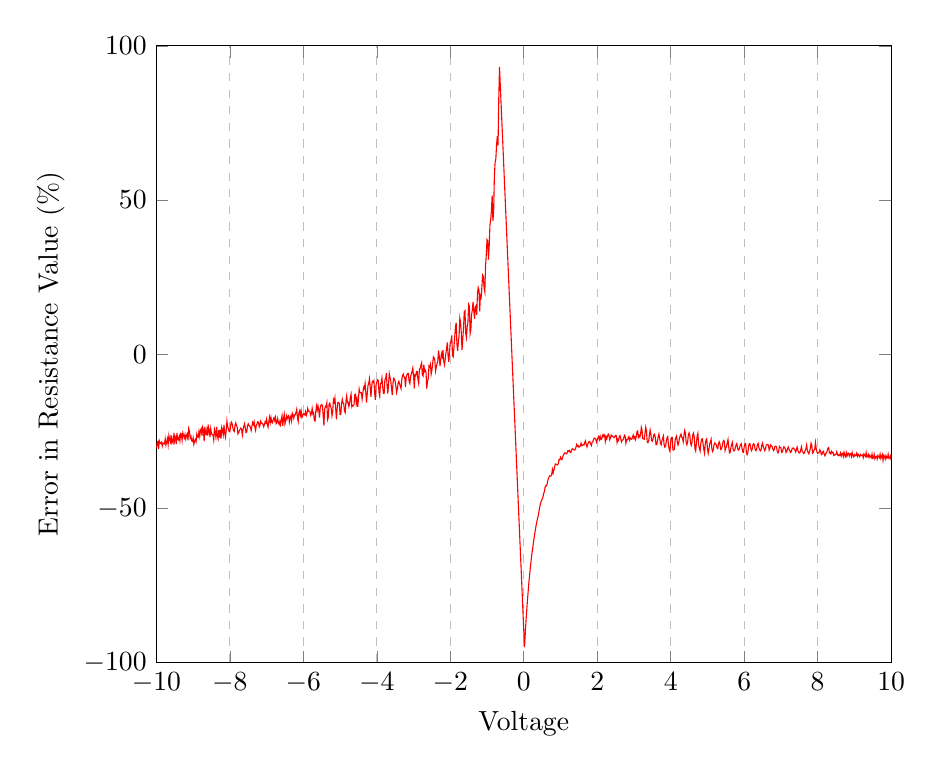
\begin{tikzpicture}

\begin{axis}[
    %title={Temperature dependence of CuSO$_4\cdot$5H$_2$O solubility},
    xlabel={Voltage},
    ylabel={Error in Resistance Value (\%)},
    % height=8cm,
    width=0.9\textwidth,
    xmin=-10, xmax=10,
    ymin=-100, ymax=100,
    xtick={-10, -8, -6, -4, -2, 0, 2, 4, 6, 8, 10},
    ytick={-100, -50, 0, 50, 100},
    legend pos=south east,
    xmajorgrids=true,
    grid style=dashed,
]

\addplot[color=red]
  coordinates {
  (-10.0,-30.364475134465007)
(-9.98,-28.849073474295984)
(-9.96,-28.423593785412805)
(-9.94,-30.78228828365822)
(-9.92,-28.13613833876788)
(-9.9,-28.85477695538019)
(-9.88,-28.998504678702663)
(-9.86,-28.570798792364048)
(-9.84,-29.847182664035323)
(-9.82,-28.860572428094823)
(-9.8,-29.005459245960196)
(-9.78,-29.150346063825594)
(-9.76,-27.542222126691584)
(-9.74,-29.440119699556366)
(-9.72,-28.43066236196965)
(-9.7,-27.38755644646339)
(-9.68,-29.30465641456027)
(-9.66,-26.461344952595102)
(-9.64,-27.836705581846076)
(-9.62,-28.581575497825117)
(-9.6,-26.293475219249117)
(-9.58,-28.878533603863264)
(-9.56,-28.43557109568967)
(-9.54,-26.75414099912882)
(-9.52,-29.323970762920492)
(-9.5,-26.43246920455763)
(-9.48,-27.214806779008494)
(-9.46,-29.18415298799418)
(-9.44,-25.614599333110622)
(-9.42,-27.675472558888192)
(-9.4,-27.829027818848083)
(-9.38,-26.730106262787256)
(-9.36,-28.136138338767893)
(-9.34,-25.751275673019023)
(-9.32,-25.91026651740229)
(-9.3,-27.981259326566942)
(-9.28,-25.569571850866733)
(-9.26,-26.387239050552058)
(-9.24,-27.190561211646404)
(-9.22,-26.050803067348195)
(-9.2,-27.505753587353578)
(-9.18,-26.371623878335836)
(-9.16,-25.870160718819125)
(-9.14,-27.978542150914286)
(-9.12,-24.14370157981056)
(-9.1,-25.004456293897682)
(-9.08,-27.17367590580495)
(-9.06,-26.679438440229397)
(-9.04,-28.136138338767893)
(-9.02,-28.295129183151147)
(-9.0,-27.165005073075555)
(-8.98,-29.239311653742938)
(-8.96,-28.136138338767868)
(-8.94,-27.650571705921724)
(-8.92,-28.456959149755523)
(-8.9,-25.973568427665995)
(-8.88,-26.81753537250674)
(-8.86,-26.98236074328939)
(-8.84,-25.08531402296087)
(-8.82,-26.63897455415889)
(-8.8,-24.714049688233008)
(-8.78,-24.162895987305532)
(-8.76,-26.457076150421344)
(-8.74,-23.775467121460103)
(-8.72,-24.68114498967019)
(-8.7,-28.30096370955053)
(-8.68,-23.556578527022698)
(-8.66,-25.91178071592022)
(-8.64,-26.082885148446955)
(-8.62,-24.084989274531765)
(-8.6,-26.425094013500463)
(-8.58,-23.689117196364894)
(-8.56,-24.61340002204082)
(-8.54,-26.93840731108069)
(-8.52,-24.22275973345327)
(-8.5,-25.86858930576784)
(-8.48,-26.04301615446015)
(-8.46,-26.217443003152454)
(-8.44,-27.793929473714396)
(-8.42,-24.363285601553198)
(-8.4,-25.290044807629975)
(-8.38,-26.915150397921693)
(-8.36,-23.60352448017542)
(-8.34,-26.550906096240713)
(-8.32,-27.438430943998636)
(-8.3,-24.611975254268625)
(-8.28,-27.07931684374978)
(-8.26,-24.517357919407768)
(-8.24,-27.43159067542247)
(-8.22,-23.797607990798753)
(-8.2,-24.682558074884554)
(-8.18,-26.149951207427304)
(-8.16,-23.003005362965588)
(-8.14,-25.613958046486584)
(-8.12,-26.912004422694803)
(-8.1,-24.754746709413123)
(-8.08,-21.7860988385297)
(-8.06,-23.5450468598824)
(-8.04,-24.214920283800346)
(-8.02,-25.11068470334179)
(-8.0,-25.219706908187177)
(-7.98,-23.250319050236566)
(-7.96,-22.023399833232325)
(-7.94,-22.472953588290345)
(-7.92,-23.82738432053554)
(-7.9,-24.8246150524717)
(-7.88,-25.09428176051468)
(-7.86,-23.086880084792426)
(-7.84,-22.352167113552944)
(-7.82,-23.143408343704163)
(-7.8,-23.757056452990955)
(-7.78,-25.888011171210778)
(-7.76,-25.525698919449624)
(-7.74,-24.752937059261825)
(-7.72,-24.374453104592163)
(-7.7,-23.99014631985065)
(-7.68,-24.436684343063707)
(-7.66,-26.249038005755885)
(-7.64,-24.416312900356086)
(-7.62,-23.433637324022826)
(-7.6,-22.595613856949537)
(-7.58,-23.920660420092265)
(-7.56,-25.454062272377232)
(-7.54,-25.240960689060397)
(-7.52,-23.23632958913843)
(-7.5,-22.64940263214109)
(-7.48,-23.20833068199769)
(-7.46,-23.23820045922228)
(-7.44,-23.879964299606073)
(-7.42,-24.770054525064577)
(-7.4,-23.32863663594035)
(-7.38,-22.18965682806734)
(-7.36,-22.85326402761546)
(-7.34,-21.9703040542243)
(-7.32,-23.717594640339456)
(-7.3,-24.71208522861733)
(-7.28,-23.063395162680912)
(-7.26,-22.63765782020386)
(-7.24,-21.924616082334868)
(-7.22,-22.046712560983185)
(-7.2,-23.63934416161878)
(-7.18,-23.125368485153963)
(-7.16,-21.754067899266726)
(-7.14,-22.350488459261907)
(-7.12,-22.474137116973825)
(-7.1,-22.69190639473515)
(-7.08,-23.558272151213423)
(-7.06,-22.94063436690481)
(-7.04,-21.925681158167563)
(-7.02,-22.33923816781873)
(-7.0,-21.10303769940012)
(-6.98,-22.686536005641145)
(-6.96,-23.66109933422228)
(-6.94,-21.975093878449492)
(-6.92,-20.508644070376235)
(-6.9,-22.13243632812474)
(-6.88,-20.56179816367657)
(-6.86,-22.094486252204113)
(-6.84,-22.321616029894486)
(-6.82,-21.254573179691015)
(-6.8,-20.669763101237272)
(-6.78,-21.514661394466216)
(-6.76,-20.517064000338813)
(-6.74,-22.576338299759513)
(-6.72,-22.209221913099253)
(-6.7,-20.911978789379905)
(-6.68,-22.17078536040361)
(-6.66,-22.80430344132163)
(-6.64,-21.825681285946718)
(-6.62,-22.86985016255566)
(-6.6,-21.159992193462106)
(-6.58,-20.016202684217298)
(-6.56,-23.27035603878863)
(-6.54,-20.9304079299364)
(-6.52,-19.54801201386789)
(-6.5,-22.663062781786625)
(-6.48,-21.655817031496603)
(-6.46,-20.06877645806483)
(-6.44,-20.969387107524796)
(-6.42,-20.123616366843798)
(-6.4,-19.928844945702373)
(-6.38,-22.025265748527055)
(-6.36,-20.760374451207298)
(-6.34,-20.123267368125596)
(-6.32,-21.585012828213568)
(-6.3,-19.153155631113872)
(-6.28,-19.753724887528858)
(-6.26,-20.797927112796998)
(-6.24,-19.693678945901073)
(-6.22,-19.721045342517286)
(-6.2,-18.93086930501471)
(-6.18,-17.877465779139346)
(-6.16,-20.609507203516884)
(-6.14,-21.876042740799374)
(-6.12,-19.034088113633917)
(-6.1,-18.336520839508964)
(-6.08,-19.799508278213796)
(-6.06,-18.38549444020491)
(-6.04,-20.560445747832723)
(-6.02,-20.23959306773281)
(-6.0,-19.314526577957956)
(-5.98,-19.462913655515724)
(-5.96,-19.732268459343437)
(-5.94,-18.660187067888945)
(-5.92,-19.91075658236181)
(-5.9,-19.207929915916633)
(-5.88,-17.59760012323618)
(-5.86,-18.51350051570816)
(-5.84,-18.539411470963596)
(-5.82,-18.692131635231167)
(-5.8,-19.844154300933415)
(-5.78,-19.25094859993748)
(-5.76,-17.608311471198856)
(-5.74,-19.433873840728054)
(-5.72,-19.082423483809507)
(-5.7,-21.588052934719936)
(-5.68,-21.74334082902637)
(-5.66,-18.519740183779287)
(-5.64,-16.807844874928346)
(-5.62,-18.17769397566359)
(-5.6,-16.851730309318224)
(-5.58,-18.09633413609575)
(-5.56,-20.595574158098074)
(-5.54,-17.469777445434097)
(-5.52,-16.521776858164717)
(-5.5,-16.402022179192755)
(-5.48,-16.706014825813863)
(-5.46,-19.857703294459284)
(-5.44,-23.16442463893421)
(-5.42,-17.895841019418622)
(-5.4,-16.938173593610127)
(-5.38,-17.103864550294002)
(-5.36,-15.823798403801536)
(-5.34,-21.23295950924067)
(-5.32,-20.483414301631676)
(-5.3,-16.327226097423065)
(-5.28,-15.90399167302624)
(-5.26,-16.95871873065006)
(-5.24,-17.564221737115528)
(-5.22,-19.9809390205564)
(-5.2,-18.62106257874411)
(-5.18,-14.776830722256785)
(-5.16,-15.569780015492318)
(-5.14,-14.17745145475533)
(-5.12,-17.575499169912977)
(-5.1,-21.147656094603327)
(-5.08,-17.777383504716404)
(-5.06,-15.669958254676597)
(-5.04,-15.69044162648746)
(-5.02,-16.025003366064904)
(-5.0,-19.651317462844233)
(-4.98,-19.54091028036511)
(-4.96,-16.091159642252517)
(-4.94,-14.661664277286857)
(-4.92,-15.816619196842375)
(-4.9,-16.158828061895857)
(-4.88,-18.518669863658754)
(-4.86,-19.003161485717047)
(-4.84,-15.248272309852961)
(-4.82,-13.576892912390514)
(-4.8,-15.784537115743614)
(-4.78,-15.641144710046762)
(-4.76,-16.972820022459977)
(-4.74,-16.017084745009804)
(-4.72,-13.821791910311088)
(-4.7,-12.948414997992009)
(-4.68,-17.080159621655255)
(-4.66,-16.61215255444678)
(-4.64,-16.804311849272203)
(-4.62,-16.327862682738814)
(-4.6,-13.189662909225907)
(-4.58,-13.018898940686285)
(-4.56,-16.06065338749527)
(-4.54,-14.68045712813969)
(-4.52,-17.1365676763344)
(-4.5,-14.53821948320705)
(-4.48,-11.357351254867854)
(-4.46,-12.523792846862658)
(-4.44,-12.53411574126353)
(-4.42,-12.544529586275887)
(-4.4,-14.632561741516914)
(-4.38,-12.759502750499818)
(-4.36,-10.784044179108188)
(-4.34,-11.193291682873753)
(-4.32,-9.541992314533)
(-4.3,-12.410826206548165)
(-4.28,-15.686039498335113)
(-4.26,-12.830281697935986)
(-4.24,-10.170172923459852)
(-4.22,-9.52699993723164)
(-4.2,-7.979201531349123)
(-4.18,-10.597934004776732)
(-4.16,-13.895833954284099)
(-4.14,-10.602047092097067)
(-4.12,-8.842638533166147)
(-4.1,-9.061162712638371)
(-4.08,-8.602071203919259)
(-4.06,-12.539784668884192)
(-4.04,-14.809271974360982)
(-4.02,-9.946158392096926)
(-4.0,-9.033086504769472)
(-3.98,-8.32750980394108)
(-3.96,-8.553697886092792)
(-3.94,-12.609995387267114)
(-3.92,-13.692911240186923)
(-3.9,-9.473817674804508)
(-3.88,-9.470200244941351)
(-3.86,-7.781081777807197)
(-3.84,-10.63561244199116)
(-3.82,-12.684493783108564)
(-3.8,-12.697354759372747)
(-3.78,-8.227906392075202)
(-3.76,-7.967261632754507)
(-3.74,-6.155432048530674)
(-3.72,-10.4110035590538)
(-3.7,-12.76368499128646)
(-3.68,-9.6792995514569)
(-3.66,-6.331291424462404)
(-3.64,-7.632607186834428)
(-3.62,-8.656187073855248)
(-3.6,-10.912568188555227)
(-3.58,-13.317848804848042)
(-3.56,-9.406746631024676)
(-3.54,-7.826786130158803)
(-3.52,-8.081107177493807)
(-3.5,-8.868291371625936)
(-3.48,-10.683486221040084)
(-3.46,-12.447548821174959)
(-3.44,-11.202699671466053)
(-3.42,-9.375218701543576)
(-3.4,-8.829429235750297)
(-3.38,-9.635471571813792)
(-3.36,-10.436730273835348)
(-3.34,-11.233247800105294)
(-3.32,-8.235376647965154)
(-3.3,-7.072592679441225)
(-3.28,-6.462910218713757)
(-3.26,-7.327456876733896)
(-3.24,-7.603606435558696)
(-3.22,-10.724678028870594)
(-3.2,-7.570595934106594)
(-3.18,-6.647434606732794)
(-3.16,-6.316087933377268)
(-3.14,-6.290479395237192)
(-3.12,-9.0035517925957)
(-3.1,-9.586862358027782)
(-3.08,-7.15574919605918)
(-3.06,-6.503649369315356)
(-3.04,-5.507725151321097)
(-3.02,-4.476733179172099)
(-3.0,-7.072592679441225)
(-2.98,-11.065486814588166)
(-2.96,-6.703056790681106)
(-2.94,-7.007150843299992)
(-2.92,-5.646368682195247)
(-2.9,-5.61358749204115)
(-2.88,-8.258900006937731)
(-2.86,-9.537568507427896)
(-2.84,-4.8071981726216295)
(-2.82,-4.766875054194286)
(-2.8,-3.6308368527538604)
(-2.78,-2.8299925008631988)
(-2.76,-6.793111755168879)
(-2.74,-7.119348607652832)
(-2.72,-3.424059427593207)
(-2.7,-5.626251709471431)
(-2.68,-5.218922612154476)
(-2.66,-5.926244085198107)
(-2.64,-11.179496823196256)
(-2.62,-8.777462426149151)
(-2.6,-8.048208504328969)
(-2.58,-3.833629104782754)
(-2.56,-4.181517785023836)
(-2.54,-3.318745434571202)
(-2.52,-6.45819659798299)
(-2.5,-5.242798442468189)
(-2.48,-3.140012543556703)
(-2.46,-0.9052131801395746)
(-2.44,-1.2681179879468818)
(-2.42,-2.077395709357144)
(-2.4,-5.442287287852476)
(-2.38,-4.127807873468359)
(-2.36,-3.1970813239110885)
(-2.34,-2.2317230887888617)
(-2.32,1.1675722415403378)
(-2.3,-0.6689412134411765)
(-2.28,-3.844128763140131)
(-2.26,-1.9249230951784102)
(-2.24,0.10886201564672682)
(-2.22,-0.7849671094929733)
(-2.2,1.3464715735324706)
(-2.18,-2.085488486571241)
(-2.16,-3.4664544849120738)
(-2.14,-1.9204949266347304)
(-2.12,0.23117547487636614)
(-2.1,1.9689928976942328)
(-2.08,3.803355732890834)
(-2.06,-0.5110517324340313)
(-2.04,-2.525081257371342)
(-2.02,0.8090281636728314)
(-2.0,3.8495110711446845)
(-1.98,4.013483983362254)
(-1.96,6.064133174710062)
(-1.94,-0.41722026943550317)
(-1.92,-0.8774321914039818)
(-1.9,2.201599667919929)
(-1.88,5.550046814934673)
(-1.86,8.495765170366653)
(-1.84,10.191254547222584)
(-1.82,3.474864100824737)
(-1.8,1.0585554611076686)
(-1.78,3.829280646910038)
(-1.76,6.107715204503794)
(-1.74,11.645642223699904)
(-1.72,10.36235897974931)
(-1.7,6.790703517565189)
(-1.68,1.2846372406627227)
(-1.66,5.0123330613074835)
(-1.64,8.324203239357232)
(-1.62,13.690874893746141)
(-1.6,14.069621684495438)
(-1.58,6.715132917995059)
(-1.56,5.364308450678679)
(-1.54,8.927506848717993)
(-1.52,10.113981577694364)
(-1.5,16.159259150698468)
(-1.48,15.607081802851663)
(-1.46,6.627274416055773)
(-1.44,7.795792491848186)
(-1.42,12.883499512112383)
(-1.4,14.328870824687456)
(-1.38,16.94826543926924)
(-1.36,14.176228807565039)
(-1.34,11.455526187559073)
(-1.32,15.121720136925255)
(-1.3,15.622549702477407)
(-1.28,12.727626135266057)
(-1.26,19.773102768720218)
(-1.24,21.603696042477914)
(-1.22,20.829535869216052)
(-1.2,13.82871435253239)
(-1.18,18.966549888122742)
(-1.16,18.412044782712012)
(-1.14,21.7669475234908)
(-1.12,25.604751967197203)
(-1.1,25.07950605594198)
(-1.08,21.57420205847538)
(-1.06,20.22678876405626)
(-1.04,28.504842035215617)
(-1.02,32.217061497937884)
(-1.0,37.14477416265672)
(-0.98,36.69756294256108)
(-0.96,30.661566656785656)
(-0.94,35.32057283965984)
(-0.92,41.99903936497758)
(-0.9,43.60007880796826)
(-0.88,46.66094216577983)
(-0.86,51.47774761926376)
(-0.84,43.182267066971015)
(-0.82,46.15170278325975)
(-0.8,57.59618785357921)
(-0.78,62.19274333264193)
(-0.76,63.326958320982094)
(-0.74,67.86381827434269)
(-0.72,70.65296964408682)
(-0.7,67.68234387620826)
(-0.68,82.88707308996199)
(-0.66,93.11949794956513)
(0.02,-95.05069823269751)
(0.04,-90.83369111463875)
(0.06,-86.7572736496501)
(0.08,-83.24851709528389)
(0.1,-79.94869931327229)
(0.12,-76.96671100601536)
(0.14,-74.01616572166193)
(0.16,-71.65133662278812)
(0.18,-69.14242581340224)
(0.2,-67.09530143716478)
(0.22,-64.89775851360776)
(0.24,-63.272302387785984)
(0.26,-61.52264408583123)
(0.28,-59.82052463030152)
(0.3,-58.088727647026374)
(0.32,-56.77361704587541)
(0.34,-55.282370122952194)
(0.36,-54.12945000346887)
(0.38,-53.11080454795981)
(0.4,-52.026794618670145)
(0.42,-50.61711076944129)
(0.44,-49.326764213233766)
(0.46,-48.21839541953826)
(0.48,-47.608363308943765)
(0.5,-47.03430007279472)
(0.52,-46.49311560160265)
(0.54,-45.312168408870704)
(0.56,-44.59834453429241)
(0.58,-43.244771563841745)
(0.6,-42.72274575353444)
(0.62,-42.760027967672265)
(0.64,-41.98679179718901)
(0.66,-40.71231412948351)
(0.68,-40.11344861563989)
(0.7,-39.537616390790284)
(0.72,-39.5537612195244)
(0.74,-39.569025421236624)
(0.76,-39.044045912347755)
(0.78,-37.43994185740954)
(0.8,-38.577896016040924)
(0.82,-37.57588287901448)
(0.84,-36.590710298912846)
(0.86,-35.621957261812895)
(0.88,-35.731505831418445)
(0.9,-35.835837802471325)
(0.92,-35.9353171237078)
(0.94,-35.54195614355136)
(0.96,-34.170508401924785)
(0.98,-34.30355930223183)
(1.0,-33.45938735071101)
(1.02,-34.0817096272871)
(1.04,-34.209140732674825)
(1.06,-33.41285545375345)
(1.08,-32.627629692594894)
(1.1,-32.31999329849714)
(1.12,-32.02067140153718)
(1.14,-32.18145505479752)
(1.16,-32.33597440987885)
(1.18,-32.05179746774528)
(1.2,-31.340259559332374)
(1.22,-31.504756854138137)
(1.24,-31.241366929068036)
(1.26,-31.815914387686394)
(1.28,-31.963207894691482)
(1.3,-31.306602823822228)
(1.32,-30.65767734442515)
(1.34,-30.82070788358402)
(1.36,-30.97821196378836)
(1.38,-31.130465907985894)
(1.4,-30.90013301804605)
(1.42,-30.295981175580877)
(1.44,-29.31423443157498)
(1.46,-29.865482603342997)
(1.48,-29.65706662789448)
(1.5,-30.18407222030559)
(1.52,-29.978801458286654)
(1.54,-29.777698630521922)
(1.56,-28.86572069065856)
(1.58,-29.73706595003295)
(1.6,-29.545233665458703)
(1.62,-29.357126279614054)
(1.64,-29.51152325094458)
(1.66,-28.651907680834153)
(1.68,-28.136138338767893)
(1.7,-29.300599060130438)
(1.72,-30.08719340649365)
(1.74,-29.274253794941252)
(1.76,-28.783560515896113)
(1.78,-28.29726807343431)
(1.8,-28.45412002753439)
(1.82,-29.224984727574434)
(1.84,-29.66515667198558)
(1.86,-28.59680411864758)
(1.88,-28.440646227162947)
(1.9,-27.679376506175313)
(1.92,-27.226469203815583)
(1.94,-27.38755644646338)
(1.96,-27.54466622632976)
(1.98,-28.569053168052417)
(2.0,-27.847528452578196)
(2.02,-27.126003737103964)
(2.04,-26.698861105543237)
(2.06,-27.71506102434659)
(2.08,-26.727043012077058)
(2.1,-27.72312763956539)
(2.12,-27.58964509419577)
(2.14,-26.346425308890442)
(2.16,-26.78021642063142)
(2.18,-26.102255461563207)
(2.2,-26.25909717597449)
(2.22,-28.2653898885183)
(2.24,-26.829522672200024)
(2.26,-27.494496716792604)
(2.28,-26.59067894820376)
(2.3,-25.94673753546871)
(2.32,-26.35858699025685)
(2.34,-27.7657060621636)
(2.36,-27.14831893448979)
(2.38,-26.277590192356705)
(2.4,-26.669528917110085)
(2.42,-26.558046782017865)
(2.44,-26.93840731108068)
(2.46,-27.068853264591176)
(2.48,-26.71777264808567)
(2.5,-26.36899419955726)
(2.52,-26.50286875555806)
(2.54,-28.697574757996257)
(2.56,-27.68416436605574)
(2.58,-28.024548491467826)
(2.6,-26.78446695955975)
(2.62,-26.451829081082757)
(2.64,-27.47683685563731)
(2.66,-28.45888023245604)
(2.68,-27.920977076309107)
(2.7,-27.815317527780238)
(2.72,-27.280616176134163)
(2.74,-26.307267607868255)
(2.76,-26.64783351146427)
(2.78,-28.85272955191408)
(2.8,-27.723127639565405)
(2.82,-27.829027818848097)
(2.84,-27.3171769523151)
(2.86,-26.8053260857821)
(2.88,-27.935960451132136)
(2.9,-27.232821641908835)
(2.92,-27.540581474172043)
(2.94,-27.643920108211496)
(2.96,-26.951569190505808)
(2.98,-26.255403667192933)
(3.0,-27.361325814118477)
(3.02,-26.877067986212598)
(3.04,-27.755906266486228)
(3.06,-26.893810943028495)
(3.08,-25.2227385416909)
(3.1,-24.940036674589095)
(3.12,-27.013265500311135)
(3.14,-26.35361435500364)
(3.16,-26.839625370652865)
(3.18,-25.99511655352392)
(3.2,-23.7518709164646)
(3.22,-24.67394708685956)
(3.24,-27.41929183840647)
(3.26,-27.513555378831477)
(3.28,-27.606429284753897)
(3.3,-25.704654297598374)
(3.32,-23.725057316083564)
(3.34,-24.992094391088994)
(3.36,-28.476725360859035)
(3.38,-28.726569127064383)
(3.4,-28.13613833876788)
(3.42,-26.326616642262046)
(3.44,-24.630584111390718)
(3.46,-25.997332932183603)
(3.48,-27.970553404064592)
(3.5,-28.21817471052729)
(3.52,-27.47683685563731)
(3.54,-26.218657111148)
(3.56,-25.97356842766598)
(3.58,-27.07692042312614)
(3.6,-29.39140229791605)
(3.62,-29.3078317354184)
(3.64,-28.13613833876788)
(3.66,-26.775686614668825)
(3.68,-25.88032205343772)
(3.7,-27.430052361747048)
(3.72,-28.90064750537673)
(3.74,-29.419421582718453)
(3.76,-28.13613833876788)
(3.78,-27.289775942329385)
(3.8,-26.59067894820376)
(3.82,-29.393016577698905)
(3.84,-30.172765997183358)
(3.86,-29.950882320112125)
(3.88,-28.284006366877424)
(3.9,-27.165005073075555)
(3.92,-26.79149227857851)
(3.94,-29.636278592133568)
(3.96,-30.92696791784485)
(3.98,-31.640016871007692)
(4.0,-28.422448544589518)
(4.02,-27.047291949961338)
(4.04,-26.9793759780237)
(4.06,-31.05688129853441)
(4.08,-31.10795216686394)
(4.1,-30.90013301804605)
(4.12,-27.996325378337474)
(4.14,-27.07931684374978)
(4.16,-26.583088283220626)
(4.18,-28.614319927768474)
(4.2,-29.479388089445113)
(4.22,-28.6098172762713)
(4.24,-27.31326969379194)
(4.26,-26.408641664219047)
(4.28,-25.92068210258346)
(4.3,-26.98142600583693)
(4.32,-27.19233527755096)
(4.34,-28.46578908033317)
(4.36,-26.380066531256563)
(4.38,-24.76966680779239)
(4.4,-25.564738392320773)
(4.42,-28.588518762894346)
(4.44,-29.408065093833923)
(4.46,-28.584486851805877)
(4.48,-26.293475219249107)
(4.5,-25.55539192551921)
(4.52,-26.443692321383793)
(4.54,-28.825931077226485)
(4.56,-29.617867445185052)
(4.58,-28.572811109278838)
(4.6,-26.211213472842022)
(4.62,-25.624766829101166)
(4.64,-26.875368835939252)
(4.66,-30.694206262139556)
(4.68,-31.41866383063493)
(4.7,-28.802666566654512)
(4.72,-26.51702187153041)
(4.74,-25.690509538778304)
(4.76,-29.323970762920492)
(4.78,-30.519971937562794)
(4.8,-31.449416539365238)
(4.82,-29.01971040837319)
(4.84,-27.657843086446864)
(4.86,-27.479574818607123)
(4.88,-29.066414865126877)
(4.9,-30.791485428451782)
(4.92,-32.11017677164708)
(4.94,-29.337683796479563)
(4.96,-27.903569207178126)
(4.98,-27.49553665459158)
(5.0,-30.579731780108077)
(5.02,-32.188611740717064)
(5.04,-30.879033822021018)
(5.06,-29.199544391387366)
(5.08,-28.474056183569907)
(5.1,-27.625257805631176)
(5.12,-30.733627314475076)
(5.14,-31.596250196530917)
(5.16,-31.023525637656668)
(5.18,-29.390211797196063)
(5.2,-28.7934297564011)
(5.22,-29.16741732031125)
(5.24,-29.323078996836283)
(5.26,-30.41165089505138)
(5.28,-30.65767734442515)
(5.3,-29.15207090689542)
(5.32,-28.45888023245604)
(5.34,-29.14456771215298)
(5.36,-30.91996081344974)
(5.38,-30.76153729630574)
(5.4,-30.002732148150525)
(5.42,-28.61031337905461)
(5.44,-28.03030054545236)
(5.46,-28.29373452662146)
(5.48,-31.24756251683798)
(5.5,-30.413514236482975)
(5.52,-29.96318566913819)
(5.54,-28.80440028554615)
(5.56,-27.720139139571177)
(5.58,-30.18796168703426)
(5.6,-32.02067140153719)
(5.62,-31.777888085114103)
(5.64,-30.214845081034937)
(5.66,-29.285560326395377)
(5.68,-28.638682825909367)
(5.7,-30.99325952341254)
(5.72,-31.398316304698316)
(5.74,-31.250239010754612)
(5.76,-30.266872781553744)
(5.78,-29.45429340999972)
(5.8,-29.01730285505002)
(5.82,-30.477447661507494)
(5.84,-31.154043290420674)
(5.86,-31.008809086693933)
(5.88,-30.039816793370054)
(5.9,-29.427965412571655)
(5.92,-29.094323160917646)
(5.94,-30.52224312048848)
(5.96,-31.710998804058764)
(5.98,-31.829648995214455)
(6.0,-30.093519784793653)
(6.02,-29.12509056346374)
(6.04,-28.982702154148875)
(6.06,-31.953905989520848)
(6.08,-32.65532076136077)
(6.1,-32.01464700162596)
(6.12,-29.78818113557781)
(6.14,-29.01478272201331)
(6.16,-29.14830540441904)
(6.18,-30.606458583372753)
(6.2,-31.326149460598153)
(6.22,-30.848821235633707)
(6.24,-29.31423443157497)
(6.26,-29.08767749065053)
(6.28,-29.571621218392995)
(6.3,-31.068463997295638)
(6.32,-31.351329247432446)
(6.34,-30.71519420130602)
(6.36,-29.379765116588953)
(6.38,-28.98211936204138)
(6.4,-30.39819693827397)
(6.42,-31.015850498637832)
(6.44,-31.37555321792188)
(6.46,-31.08067898878274)
(6.48,-29.528174400002392)
(6.5,-28.88016126705104)
(6.52,-30.025033149457382)
(6.54,-30.639070946803713)
(6.56,-31.318920090663948)
(6.58,-30.705713697112046)
(6.6,-29.50334617061059)
(6.62,-29.373698901817612)
(6.64,-29.41182819074242)
(6.66,-29.449687696962577)
(6.68,-31.106401277693664)
(6.7,-30.501173047018582)
(6.72,-29.479388089445123)
(6.74,-29.680251510350686)
(6.76,-29.959673467426594)
(6.78,-30.790201411483842)
(6.8,-31.28877119004804)
(6.82,-30.85333852573321)
(6.84,-29.858902145715238)
(6.86,-29.893900597831013)
(6.88,-30.08719340649365)
(6.9,-31.586555537734316)
(6.92,-32.063125314791485)
(6.94,-31.34151983356952)
(6.96,-29.987055268452465)
(6.98,-30.331978556194407)
(7.0,-30.364475134465007)
(7.02,-31.82644474839873)
(7.04,-31.7797214003406)
(7.06,-30.764347253234348)
(7.08,-30.033534026193166)
(7.1,-30.295981175580867)
(7.12,-30.780479568726648)
(7.14,-31.912424063004607)
(7.16,-31.5035610364188)
(7.18,-30.72200231905927)
(7.2,-30.153914152150207)
(7.22,-30.9295685311374)
(7.24,-31.32334234063878)
(7.26,-31.924369042204447)
(7.28,-31.665502495589116)
(7.3,-30.82724286300178)
(7.32,-30.49108517967506)
(7.34,-30.44821405677165)
(7.36,-30.842308861575784)
(7.38,-31.01517962280268)
(7.4,-31.75146608147873)
(7.42,-31.142839162404133)
(7.44,-30.163645407580088)
(7.46,-31.12738849013469)
(7.48,-31.784050098221282)
(7.5,-32.084304125599694)
(7.52,-31.97177244556074)
(7.54,-30.956483572159765)
(7.56,-30.06040239972776)
(7.58,-31.566825201992522)
(7.6,-31.72933142182949)
(7.62,-32.22739778977862)
(7.64,-32.0495169440825)
(7.66,-31.190352459370253)
(7.68,-30.733627314475076)
(7.7,-29.49136916520294)
(7.72,-31.337993561298028)
(7.74,-31.835013571331295)
(7.76,-32.32238270738335)
(7.78,-31.482739739658594)
(7.8,-30.626470178513543)
(7.82,-28.899873710673685)
(7.84,-29.573415571992523)
(7.86,-32.10938069023024)
(7.88,-31.936631022775362)
(7.9,-31.10139476653716)
(7.92,-30.92696791784485)
(7.94,-28.675117301227125)
(7.96,-30.57811422046023)
(7.98,-31.729331421829478)
(8.0,-32.20390409317725)
(8.02,-32.03441385341019)
(8.04,-31.86492361364315)
(8.06,-31.04491369172252)
(8.08,-31.525943134109024)
(8.1,-32.62762969259491)
(8.12,-32.46127816097169)
(8.14,-31.66216893429562)
(8.16,-31.494262715460962)
(8.18,-32.58642334989923)
(8.2,-33.03594708839734)
(8.22,-32.25677260833394)
(8.24,-32.0919472375513)
(8.26,-31.296817439609125)
(8.28,-30.486825402453054)
(8.3,-30.318919183618387)
(8.32,-32.05598533847144)
(8.34,-31.89265838015046)
(8.36,-32.34438249010131)
(8.38,-31.56600446350849)
(8.4,-32.02067140153718)
(8.42,-31.85881585725513)
(8.44,-32.9058636702656)
(8.46,-32.746872825882335)
(8.48,-32.587881981499066)
(8.5,-32.428891137115826)
(8.52,-31.665167259631954)
(8.54,-32.70642778652169)
(8.56,-32.548831598668095)
(8.58,-32.97913771159004)
(8.6,-32.82291192536999)
(8.62,-32.07604303510736)
(8.64,-33.092266729197675)
(8.66,-32.35423456670977)
(8.68,-32.19800878048971)
(8.7,-33.20346191744451)
(8.72,-31.885557208049566)
(8.74,-32.89635139752471)
(8.76,-33.31277244148375)
(8.78,-32.00811364379117)
(8.8,-33.008264553088694)
(8.82,-32.282130357685126)
(8.84,-32.12857509772523)
(8.86,-33.11829681528188)
(8.88,-32.39924877629859)
(8.9,-32.24699483210107)
(8.92,-33.226495206438486)
(8.94,-31.94248694370603)
(8.96,-32.92706244951668)
(8.98,-33.332905194435504)
(9.0,-32.627629692594894)
(9.02,-33.03594708839736)
(9.04,-32.88746803537828)
(9.06,-32.17848055721218)
(9.08,-33.14304673319799)
(9.1,-32.44203087632106)
(9.12,-32.84852270999623)
(9.14,-33.24840492035959)
(9.16,-32.55399868679445)
(9.18,-32.9562754014115)
(9.2,-32.81021064193745)
(9.22,-32.6641458824634)
(9.24,-33.59779182502153)
(9.26,-32.3720163635153)
(9.28,-32.77251651046028)
(9.3,-33.16660865505412)
(9.32,-31.933822085093155)
(9.34,-33.4118583416758)
(9.36,-33.26927131457018)
(9.38,-32.59169776176426)
(9.4,-33.51178153389941)
(9.42,-32.84151023325331)
(9.44,-33.228852944681975)
(9.46,-33.61014342624454)
(9.48,-32.413749151936464)
(9.5,-33.84625137774175)
(9.52,-33.706980328010694)
(9.54,-32.521531471638355)
(9.56,-33.94052716525201)
(9.58,-33.28916717881747)
(9.6,-33.1498961290864)
(9.62,-34.033363627762135)
(9.64,-32.87135402962426)
(9.66,-33.24952849543248)
(9.68,-33.62192930527416)
(9.7,-32.453540880431056)
(9.72,-33.852581880002255)
(9.74,-33.21049498278617)
(9.76,-32.558529825612936)
(9.78,-34.437633671002786)
(9.8,-32.79906066029821)
(9.82,-33.17205288699817)
(9.84,-34.03541056468992)
(9.86,-32.89984128979654)
(9.88,-33.767261827148)
(9.9,-33.633187458377044)
(9.92,-32.49152389399408)
(9.94,-33.858631026606744)
(9.96,-33.72554980130816)
(9.98,-33.09688998329323)
(10.0,-34.43078315581012)

};


\end{axis}
\end{tikzpicture}

% \caption{Percentage Error vs Voltage of 14um gap at $300\degree C$}
\caption{Close}
\label{fig:err_res_sub2}
\end{center}
% \end{figure}

  \end{subfigure}
  \caption{Percentage Error vs Voltage of 14um gap at $300\degree C$}
  \label{fig:err_res}
  \end{figure*}



  \section{Fabrication}
\label{sec:fab}

\subsection{Cleanrooms}
\label{sec:fab:cleanrooms}

% \hl{3.125\%
%
% Briefly describe why fabrication takes place within a cleanroom. [100 words max]
%
% The clean rooms minimise contamination
%
% there are different scales of cleanroom and so the results from fabrication can be more predictable, e.g. in terms of the likelihood of devices having errors. <-- is this true?
%
% A cleanroom is a controlled environment }

Fabrication of electronic devices takes place in a cleanroom. Cleanrooms are controlled environments where atmospheric conditions are controlled. The class of a cleanroom specifies the number of particles of various sizes for a give volume of air. Guaranteeing the number and size of contamination particles in a fabrication process gives a reasonable approximation as to the feasibility and the probability of success. As devices become smaller, the need for better cleanrooms increases since smaller particles will have a greater effect on the performance and yield of the devices.


\subsection{Cleans}
\label{sec:fab:cleans}

\hl{3.125\%

Briefly describe why we carry out steps 1 and 9. [100 words max]}

Prior to spinning the photoresist for both the p-contact and the mesa etch, the substrates were cleaned to ensure that there was no contamination on the surface and to ensure that the photoresist was deposited correctly.

The cleaning process comprised of 3 minutes in an ultrasonic bath each for OptiClear, acetone and isopropanol (IPA) to remove any particles or organic compounds on the substrate surface. Special attention was given when transferring the substrate from the acetone to the IPA so that the acetone did not dry out and leave a residue. The substrate was then rinsed briefly in RO water before being dried thoroughly by the N2 gun. Lastly the substrate was ashed in an oxygen plasma for 3 minutes at 150W.

\hl{too many words.}


\subsection{Photolithography}
\label{sec:fab:photolithography}

9.375\%

\hl{Briefly describe the processes carried out in steps 2 and 10. Comment on the exposure parameters and choice of developer. [250 words max + Figures]}

Vacuum chuck, suit
Spin Microposit S1818 at 4000rpm for 30 seconds. According to the S1800 series datasheet \cite{s18}, the resist thickness will be the desired $1.8\mu m$.

After spinning the back of the sample was cleaned with cotton bud soaked with acetone. This removes any unwanted photoresist and stops the back of the sample contaminating or sticking to the hotplate.

After spinning the substrate is baked on a hotplate at $115\degree C$ for 120 seconds. \hl{This hardens the photoresist enough so that it does not stick to the photomask and so that the structure does not colapse and distort after exposing.}

The SUSS MicroTec MJB4 mask aligner was used to align the masks on the substrate


\subsection{Etching}
\label{sec:fab:etching}

% \hl{9.375\% In step 11, describe the choice of this etch process. What other process choices are there? Why do you think that this one was chosen? What advantages does this process have over other options? [250 words max]}

Before etching, the depth of the resist was found to be $2022nm$ by the stylus profiler. The exposed areas of the substrate were wet etched for 60 seconds using a H$_{2}$SO$_{4}$:H$_{2}$O$_{2}$:H$_{2}$O 1:8:40 solution. The resist depth was measured again and found to be $2273nm$ giving an etch depth of $251nm$. Since the thickness of the p+ GaAs contact layer is $150nm$, the etch will have gone $101nm$ into the p-InGaAsP layer assuming the layer thicknesses are exact.

Another etching process is dry etching where the etchant is either a gas or plasma. Dry etching can have a slower etch rate and poor selectivity or etch ratio.


\subsection{Metallisation}
\label{sec:fab:metallisation}

% \hl{6.25\% What role does our choice of process flow have in the contact formation process? What role does the annealing step have? How have you measured it’s effect in your work? [100 words max]}

After developing the photoresist, the p-contact was metalised by evaporation deposition with Ti/Au 20/200$nm$. The back contact was then metalised by the same process with Ni/Au/Ge/Ni/Au 5/88/12/12/35$nm$.

After deposition, the metal was annealed by rapid thermal anneal at $400\degree C$ for 30 seconds. Annealing may be done for many reasons. It can reduce the resistance of the metal-semiconductor junction by reducing the trap density. The effect of this was not directly measured as the I-V response of contacts was not measured prior to annealing.


\subsection{Lift-Off}
\label{sec:fab:liftoff}

9.375\%

Describe the concept of the lift-off process, using schematics as required. [150 words max + Figures]

Suggest possible alternative process steps to achieve the same result as obtained in the lift-off process you have used. [50 words max]



  \section{Test}
\label{sec:test}

\subsection{Apparatus}
\label{sec:test:apparatus}

\begin{figure}
  \centering
  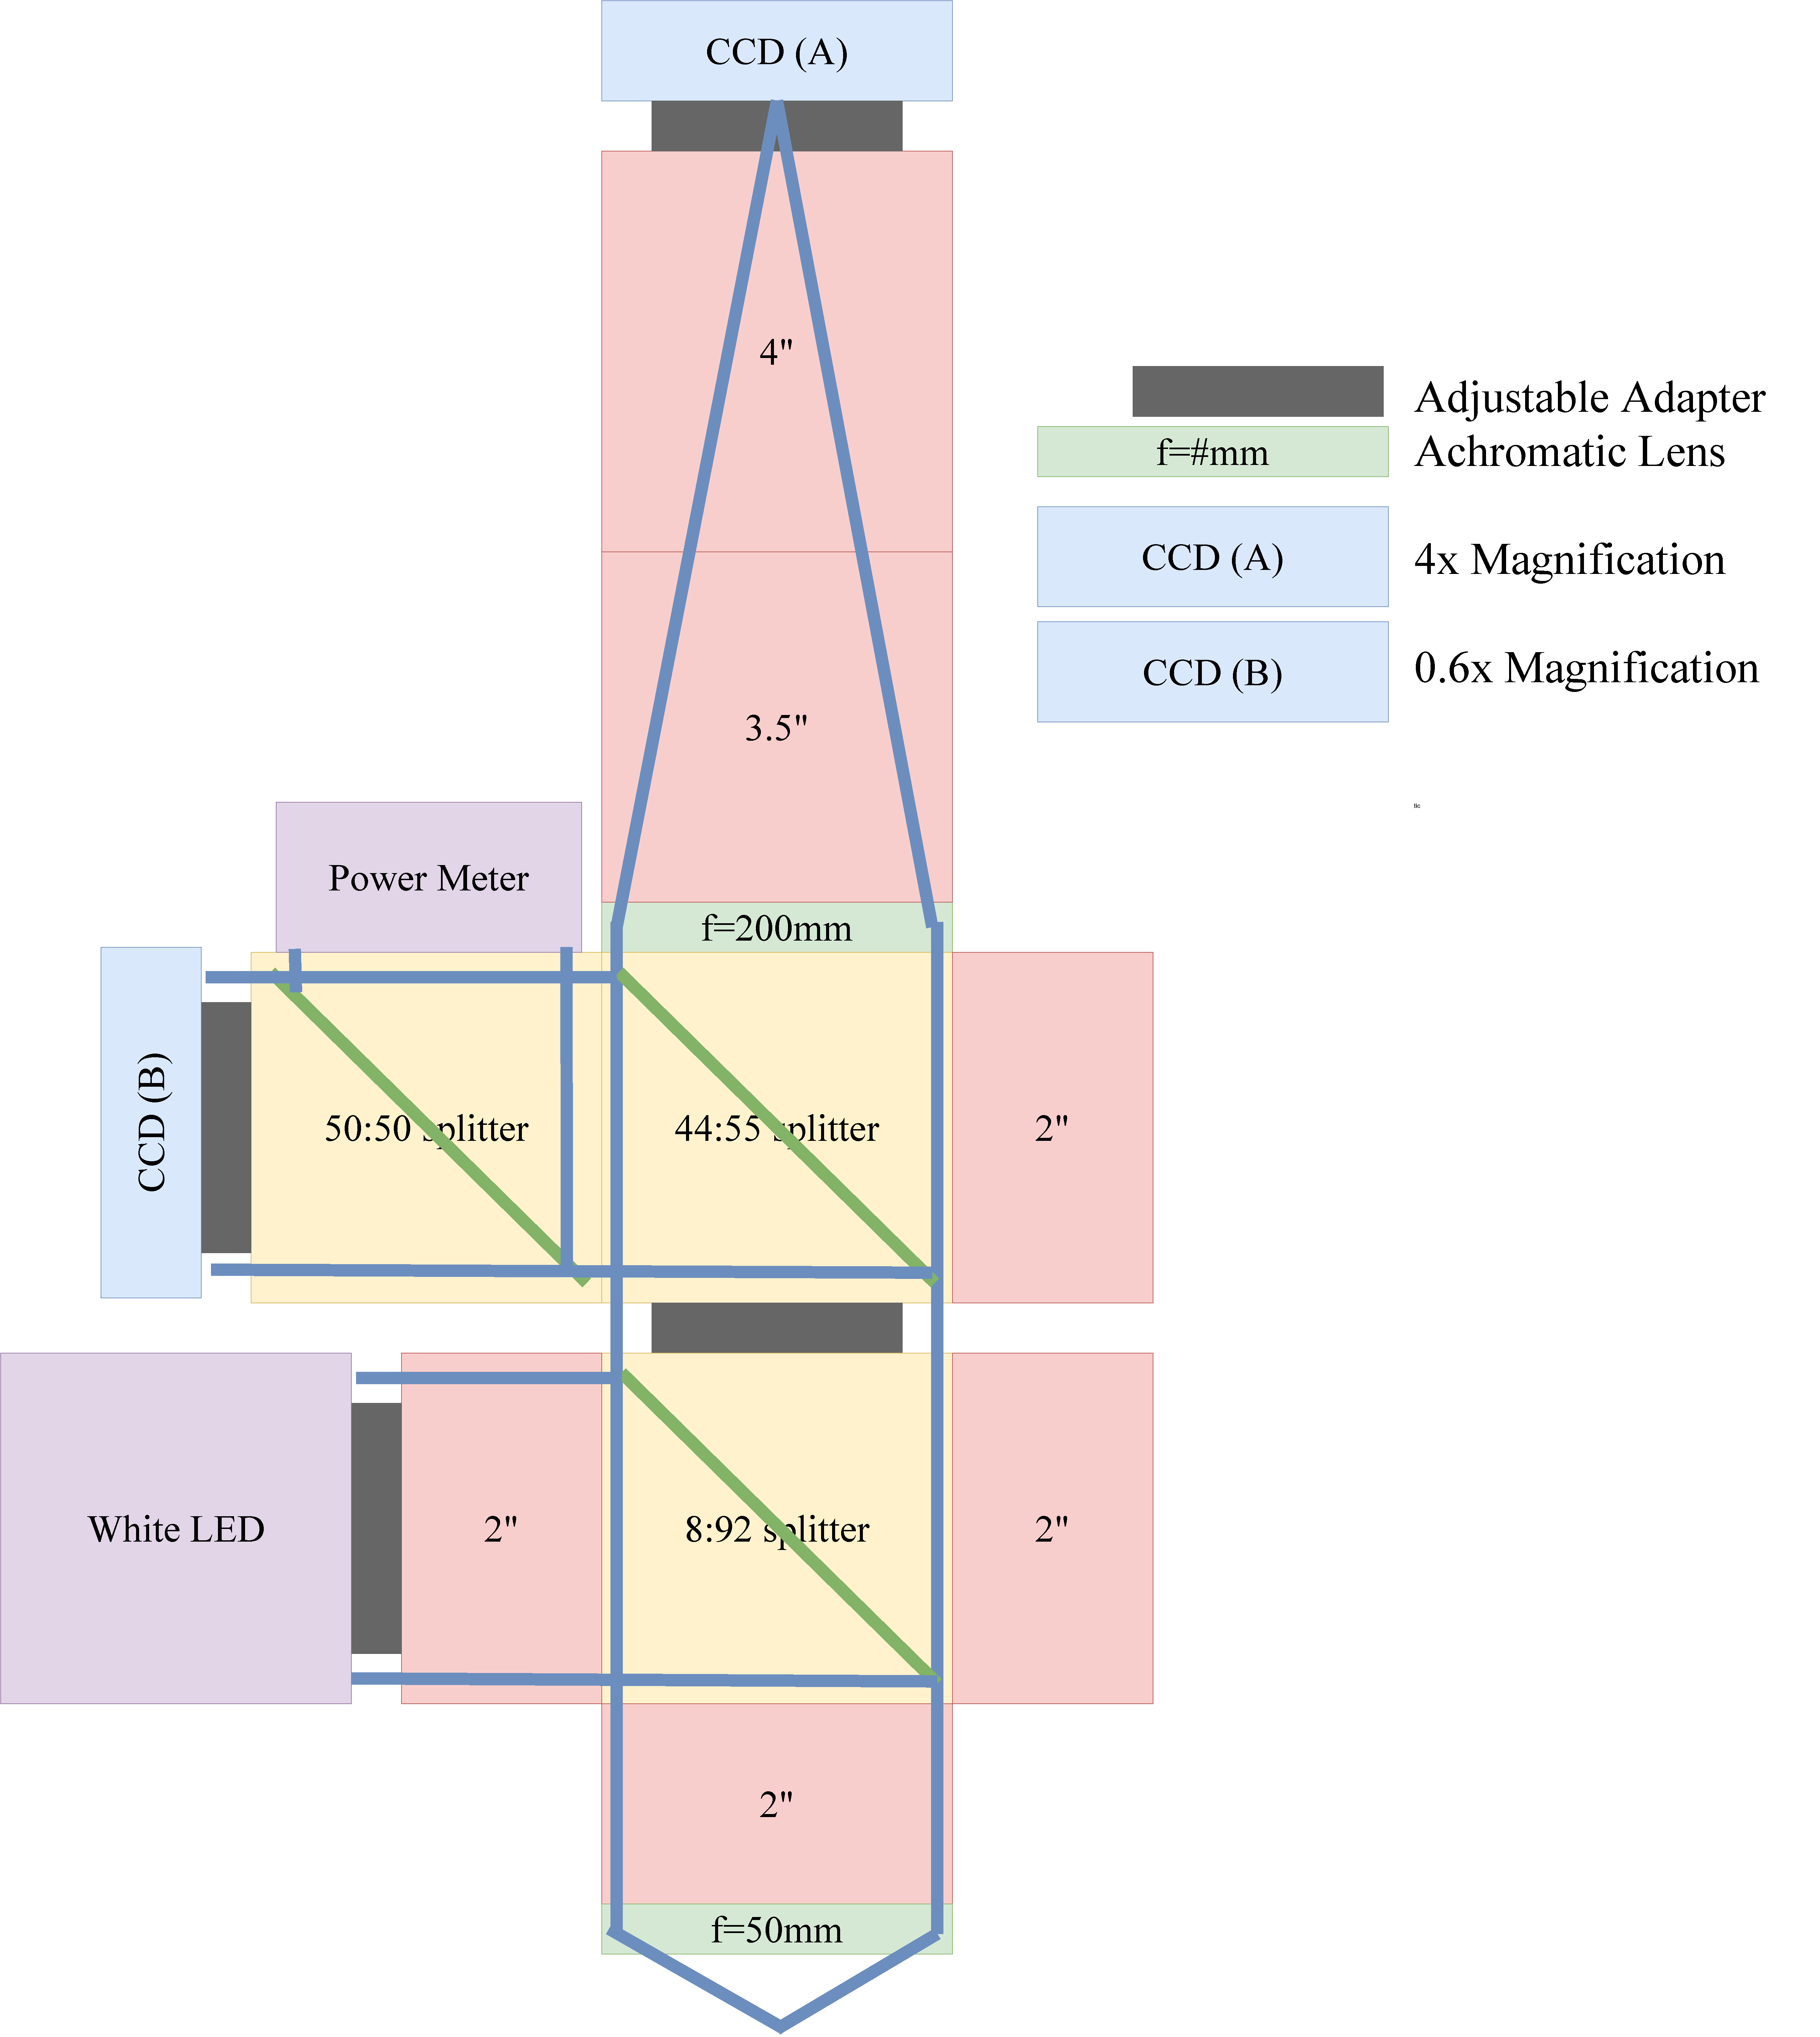
\includegraphics[width=0.6\textwidth]{Figures/angus_bruce/apparatus_microandnano1.pdf}
  \caption{Schematic of the Test Apparatus. The device to be tested is placed at the focal point below the lens with a focal length of $50mm$}
  \label{fig:apparatus}
\end{figure}

Figure \ref{fig:apparatus} shows a schematic of the apparatus used to test the LED. The measured power on the power meter will not be absolute but rather as an indication relative to other measurements on the same apparatus. This is true for two reasons. The light goes through beam splitters before being measured. Also, the light from the LED emits light in all directions so only a fraction of the light pass through the apparatus in the first place.


\subsection{I-V Characteristics}
\label{sec:test:iv}

% \hl{6.25\%
%
% Plot the forward and reverse bias VI characteristics of one of your diodes. Describe the salient features of the graphs [150 words max + Figures]}

\begin{figure*}[!htb]
  \centering
  \begin{subfigure}[t]{0.5\textwidth}
      \input{Figures/angus_bruce/plotting/iv_forward.tex}
  \end{subfigure}%
  ~
  \begin{subfigure}[t]{0.5\textwidth}
      \input{Figures/angus_bruce/plotting/iv_reverse.tex}
  \end{subfigure}
  \caption{IV}
  \label{fig:iv}
  \end{figure*}


Figure \ref{fig:iv} shows the forward and reverse current plots for this LED. The forward voltage turns on at $1.8V$ and increases to $2.5V$ at $300mA$. The reverse voltage doe not show a great deal. The voltage was limited to a range of $-5V$ to $5V$ and the first data point at $-1mA$ required more than $-5V$. As such, it shows a $-5V$ for all measured currents.


\subsection{LI Characteristics}
\label{sec:test:li}

6.25\%

Plot the output light power as a function of forward bias for one of your LEDs (or the standard). Describe the salient features of the graph. [150 words max + Figures].

\begin{figure}[!htb]
\begin{center}
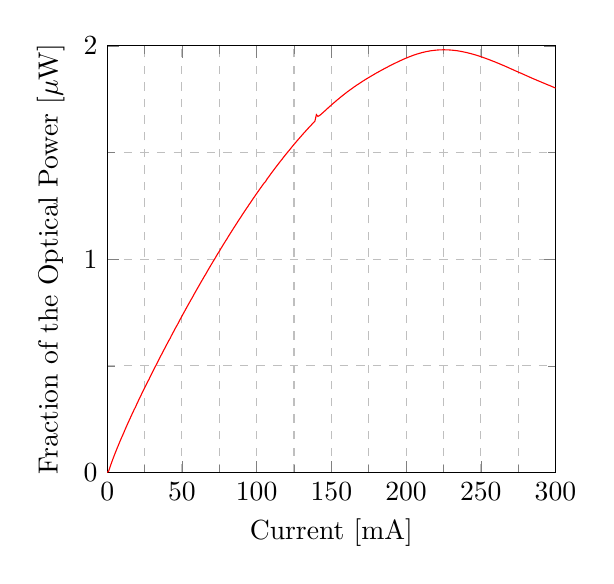
\begin{tikzpicture}

\begin{axis}[
    %title={Temperature dependence of CuSO$_4\cdot$5H$_2$O solubility},
    xlabel={Current [mA]},
    ylabel={Fraction of the Optical Power [$\mu$W]},
    height=7cm,
    width=0.6\textwidth,
    xmin=0, xmax=300,
    ymin=0, ymax=2,
    xtick={0, 50, 100, 150, 200, 250, 300},
    ytick={0, 1, 2},
    legend pos=south east,
    ymajorgrids=true,
    yminorgrids=true,
    xmajorgrids=true,
    xminorgrids=true,
    minor tick num=1,
    grid style=dashed,
]

\addplot[color=red]
  coordinates {
  (-5,-0.0014759999999999999)
  (-4,-0.000519)
  (-3,-0.0004969999999999999)
  (-2,-0.00052)
  (-1,-0.0006670000000000001)
  (0,0.000783)
  (1,0.00598)
  (2,0.027376)
  (3,0.04754)
  (4,0.066299)
  (5,0.084577)
  (6,0.102171)
  (7,0.11938700000000001)
  (8,0.136461)
  (9,0.153228)
  (10,0.169046)
  (11,0.184622)
  (12,0.20156500000000002)
  (13,0.217405)
  (14,0.233166)
  (15,0.24842799999999998)
  (16,0.26369400000000004)
  (17,0.278968)
  (18,0.29378899999999997)
  (19,0.307402)
  (20,0.323493)
  (21,0.338117)
  (22,0.352659)
  (23,0.36718999999999996)
  (24,0.381472)
  (25,0.395729)
  (26,0.409904)
  (27,0.42409)
  (28,0.436924)
  (29,0.452104)
  (30,0.466092)
  (31,0.479788)
  (32,0.49353600000000003)
  (33,0.506934)
  (34,0.520937)
  (35,0.534549)
  (36,0.548228)
  (37,0.561623)
  (38,0.5751210000000001)
  (39,0.5885130000000001)
  (40,0.601862)
  (41,0.615141)
  (42,0.627264)
  (43,0.641607)
  (44,0.6545989999999999)
  (45,0.6677379999999999)
  (46,0.680899)
  (47,0.692817)
  (48,0.706773)
  (49,0.719723)
  (50,0.732565)
  (51,0.745255)
  (52,0.758158)
  (53,0.7707909999999999)
  (54,0.783367)
  (55,0.795961)
  (56,0.8085800000000001)
  (57,0.820235)
  (58,0.8334119999999999)
  (59,0.845796)
  (60,0.858146)
  (61,0.870276)
  (62,0.882655)
  (63,0.894822)
  (64,0.906878)
  (65,0.919052)
  (66,0.930323)
  (67,0.943036)
  (68,0.954967)
  (69,0.9669690000000001)
  (70,0.978702)
  (71,0.990449)
  (72,1.0013960000000002)
  (73,1.013844)
  (74,1.025509)
  (75,1.03608)
  (76,1.048504)
  (77,1.059928)
  (78,1.0714)
  (79,1.0826360000000002)
  (80,1.093375)
  (81,1.105218)
  (82,1.116314)
  (83,1.127405)
  (84,1.138521)
  (85,1.149475)
  (86,1.1602780000000001)
  (87,1.171338)
  (88,1.182134)
  (89,1.192872)
  (90,1.203456)
  (91,1.214204)
  (92,1.2248050000000001)
  (93,1.235303)
  (94,1.245426)
  (95,1.256145)
  (96,1.266407)
  (97,1.276838)
  (98,1.2870100000000002)
  (99,1.297112)
  (100,1.3073)
  (101,1.31731)
  (102,1.327255)
  (103,1.3371870000000001)
  (104,1.346989)
  (105,1.356678)
  (106,1.364087)
  (107,1.375857)
  (108,1.384767)
  (109,1.3948280000000002)
  (110,1.4043700000000001)
  (111,1.413621)
  (112,1.422941)
  (113,1.4323000000000001)
  (114,1.4414440000000002)
  (115,1.450528)
  (116,1.4595879999999999)
  (117,1.4680039999999999)
  (118,1.477431)
  (119,1.486253)
  (120,1.494891)
  (121,1.503474)
  (122,1.51153)
  (123,1.520628)
  (124,1.529079)
  (125,1.537574)
  (126,1.5458049999999999)
  (127,1.554078)
  (128,1.562252)
  (129,1.570135)
  (130,1.578135)
  (131,1.58621)
  (132,1.593987)
  (133,1.601695)
  (134,1.609449)
  (135,1.6170930000000001)
  (136,1.6240409999999998)
  (137,1.632066)
  (138,1.639457)
  (139,1.646734)
  (140,1.6774170000000002)
  (141,1.6691939999999998)
  (142,1.67268)
  (143,1.6783130000000002)
  (144,1.684519)
  (145,1.690801)
  (146,1.696871)
  (147,1.703634)
  (148,1.709874)
  (149,1.716151)
  (150,1.722398)
  (151,1.72858)
  (152,1.73454)
  (153,1.740612)
  (154,1.7465810000000002)
  (155,1.752078)
  (156,1.758152)
  (157,1.7637779999999998)
  (158,1.76935)
  (159,1.77481)
  (160,1.780345)
  (161,1.785686)
  (162,1.790685)
  (163,1.795912)
  (164,1.800586)
  (165,1.805884)
  (166,1.810724)
  (167,1.81558)
  (168,1.82014)
  (169,1.8247879999999999)
  (170,1.829486)
  (171,1.833919)
  (172,1.838367)
  (173,1.8428360000000001)
  (174,1.847)
  (175,1.851177)
  (176,1.8554599999999999)
  (177,1.8594950000000001)
  (178,1.863529)
  (179,1.867809)
  (180,1.871826)
  (181,1.875663)
  (182,1.879619)
  (183,1.8834730000000002)
  (184,1.887251)
  (185,1.8911010000000001)
  (186,1.894866)
  (187,1.898223)
  (188,1.902201)
  (189,1.905752)
  (190,1.909238)
  (191,1.912906)
  (192,1.9163109999999999)
  (193,1.919673)
  (194,1.923133)
  (195,1.926519)
  (196,1.929702)
  (197,1.932993)
  (198,1.936236)
  (199,1.939221)
  (200,1.9421950000000001)
  (201,1.944989)
  (202,1.948101)
  (203,1.950615)
  (204,1.9534349999999998)
  (205,1.955965)
  (206,1.958264)
  (207,1.9606929999999998)
  (208,1.9627859999999997)
  (209,1.964809)
  (210,1.9668530000000002)
  (211,1.9687070000000002)
  (212,1.970365)
  (213,1.9720060000000001)
  (214,1.973468)
  (215,1.9747480000000002)
  (216,1.976153)
  (217,1.977108)
  (218,1.9779870000000002)
  (219,1.978827)
  (220,1.9795939999999999)
  (221,1.9802180000000003)
  (222,1.980754)
  (223,1.9810219999999998)
  (224,1.981178)
  (225,1.981398)
  (226,1.9812699999999999)
  (227,1.980983)
  (228,1.980873)
  (229,1.9805640000000002)
  (230,1.9799190000000002)
  (231,1.979411)
  (232,1.978652)
  (233,1.977833)
  (234,1.9770360000000002)
  (235,1.9759920000000002)
  (236,1.974693)
  (237,1.9734980000000002)
  (238,1.972148)
  (239,1.9705450000000002)
  (240,1.969024)
  (241,1.967492)
  (242,1.965611)
  (243,1.9639649999999997)
  (244,1.962118)
  (245,1.9600659999999999)
  (246,1.9580579999999999)
  (247,1.95609)
  (248,1.9538149999999999)
  (249,1.9515209999999998)
  (250,1.9492820000000002)
  (251,1.946974)
  (252,1.944379)
  (253,1.941871)
  (254,1.939252)
  (255,1.936618)
  (256,1.9339979999999999)
  (257,1.9312509999999998)
  (258,1.928425)
  (259,1.9257980000000001)
  (260,1.922955)
  (261,1.919951)
  (262,1.9172410000000002)
  (263,1.914196)
  (264,1.911133)
  (265,1.908372)
  (266,1.905305)
  (267,1.9022)
  (268,1.899225)
  (269,1.896101)
  (270,1.8926509999999999)
  (271,1.889729)
  (272,1.886485)
  (273,1.883262)
  (274,1.880274)
  (275,1.877184)
  (276,1.874037)
  (277,1.871232)
  (278,1.8680420000000002)
  (279,1.864937)
  (280,1.8617320000000002)
  (281,1.858662)
  (282,1.855412)
  (283,1.852364)
  (284,1.849227)
  (285,1.846035)
  (286,1.843167)
  (287,1.840312)
  (288,1.837189)
  (289,1.834391)
  (290,1.8313769999999998)
  (291,1.828379)
  (292,1.8254549999999998)
  (293,1.822578)
  (294,1.81952)
  (295,1.8165740000000001)
  (296,1.8140090000000002)
  (297,1.810908)
  (298,1.807922)
  (299,1.804923)
  (300,1.80201)
};
  % \addlegendentry{$16\mu m$}


\end{axis}
\end{tikzpicture}

\caption{Fraction of the optical power plotted against the forward current of the LED showing the optical power peak at $220mA$}
\label{fig:li}
\end{center}
\end{figure}


The optical power was measured against current from $0mA$ to $300mA$. As described in section \ref{sec:test:apparatus}, the power measured is not the total output power but a fraction. The results measurements are plotted in \ref{fig:li}. This figure shows the optical power increase from $0mA$ to $220mA$ before decreasing again as the current increases to $300mA$. The peak power is not of any particular interest since it is not absolute but the current at which it occurs, $200mA$, is.


\subsection{Spectral Characteristics}
\label{sec:test:spectral}

% 6.25\%
%
% Plot the emission spectra of your device as a function of current. Describe the salient features of the graph, and comment on any relationship to previous plots. Comment upon the collected power, system collection efficiency, and emitted power from the LED. [100 words max + Figures]

\begin{figure*}[htb]
  \centering
  \begin{subfigure}[t]{0.5\textwidth}
      \input{Figures/angus_bruce/plotting/spectral_far.tex}
  \end{subfigure}%
  ~
  \begin{subfigure}[t]{0.5\textwidth}
      \input{Figures/angus_bruce/plotting/spectral_close.tex}
  \end{subfigure}
  \caption{Normalised spectral characteristics for currents of $50mA$, $175mA$, and $300mA$}
  \label{fig:spectrum}
  \end{figure*}


The emission spectra of the LED are plotted in figure \ref{fig:spectrum}. The spectrum was measured at $50mA$, $175mA$ and $300mA$. All plots are normalised to better understand the differences in spectrum. The peak optical power is around a wavelength of $630nm$. The exact peak is difficult to determine due to the noise on the measured signal, see figure \ref{fig:spectral_close}, but can be estimated to be approximately $627nm$, $629nm$, and $632nm$ for $50mA$, $175mA$ and $300mA$ respectively. Even without a precise value, it is clear that there is a trend that the peak wavelength increases with the current. It is also noticeable that the lower the current, the tighter the wavelength is around its peak. 


\subsection{Contact Resistance}
\label{sec:test:contact}

\begin{figure}[!htb]
\begin{center}
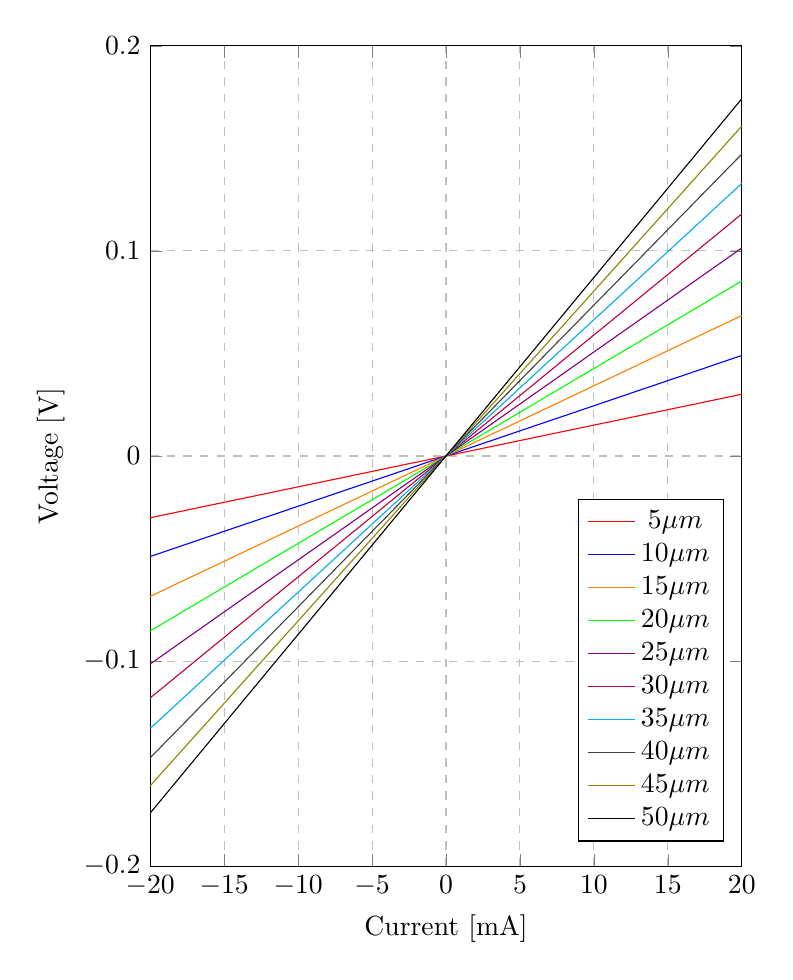
\begin{tikzpicture}

\begin{axis}[
    %title={Temperature dependence of CuSO$_4\cdot$5H$_2$O solubility},
    xlabel={Current [mA]},
    ylabel={Voltage [V]},
    height=12cm,
    width=0.75\textwidth,
    xmin=-20, xmax=20,
    ymin=-0.2, ymax=0.2,
    xtick={-20, -15, -10, -5, 0, 5, 10, 15, 20},
    ytick={-0.2, -0.1, 0, 0.1, 0.2},
    legend pos=south east,
    ymajorgrids=true,
    xmajorgrids=true,
    grid style=dashed,
]

\addplot[color=red]
  coordinates {
  (-20.000000000,-0.030106060)
  (-19.800000000,-0.029834320)
  (-19.600000000,-0.029502170)
  (-19.400000000,-0.029243770)
  (-19.200000000,-0.028904960)
  (-19.000000000,-0.028604000)
  (-18.800000000,-0.028321410)
  (-18.600000000,-0.027993270)
  (-18.400000000,-0.027730100)
  (-18.200000000,-0.027401190)
  (-18.000000000,-0.027122790)
  (-17.800000000,-0.026811620)
  (-17.600000000,-0.026515550)
  (-17.400000000,-0.026201050)
  (-17.200000000,-0.025873040)
  (-17.000000000,-0.025601530)
  (-16.800000000,-0.025270790)
  (-16.600000000,-0.025009270)
  (-16.400000000,-0.024675430)
  (-16.200000000,-0.024386870)
  (-16.000000000,-0.024089180)
  (-15.800000000,-0.023788190)
  (-15.600000000,-0.023492090)
  (-15.400000000,-0.023174160)
  (-15.200000000,-0.022900680)
  (-15.000000000,-0.022555040)
  (-14.800000000,-0.022285900)
  (-14.600000000,-0.021952910)
  (-14.400000000,-0.021677930)
  (-14.200000000,-0.021400330)
  (-14.000000000,-0.021074900)
  (-13.800000000,-0.020809100)
  (-13.600000000,-0.020466820)
  (-13.400000000,-0.020197590)
  (-13.200000000,-0.019878860)
  (-13.000000000,-0.019578650)
  (-12.800000000,-0.019280900)
  (-12.600000000,-0.018967320)
  (-12.400000000,-0.018688730)
  (-12.200000000,-0.018350630)
  (-12.000000000,-0.018089970)
  (-11.800000000,-0.017764520)
  (-11.600000000,-0.017494540)
  (-11.400000000,-0.017169810)
  (-11.200000000,-0.016848560)
  (-11.000000000,-0.016563480)
  (-10.800000000,-0.016233800)
  (-10.600000000,-0.015964600)
  (-10.400000000,-0.015660120)
  (-10.200000000,-0.015387690)
  (-10.000000000,-0.015047020)
  (-9.800000000,-0.014755250)
  (-9.600000000,-0.014452450)
  (-9.400000000,-0.014156350)
  (-9.200000000,-0.013884710)
  (-9.000000000,-0.013545790)
  (-8.800000000,-0.013270000)
  (-8.600000000,-0.012938530)
  (-8.400000000,-0.012656890)
  (-8.200000000,-0.012359900)
  (-8.000000000,-0.012042070)
  (-7.800000000,-0.011768720)
  (-7.600000000,-0.011444020)
  (-7.400000000,-0.011175730)
  (-7.200000000,-0.010848550)
  (-7.000000000,-0.010570180)
  (-6.800000000,-0.010258150)
  (-6.600000000,-0.009958734)
  (-6.400000000,-0.009645030)
  (-6.200000000,-0.009322094)
  (-6.000000000,-0.009053774)
  (-5.800000000,-0.008728319)
  (-5.600000000,-0.008459984)
  (-5.400000000,-0.008136192)
  (-5.200000000,-0.007836758)
  (-5.000000000,-0.007551670)
  (-4.800000000,-0.007221994)
  (-4.600000000,-0.006941887)
  (-4.400000000,-0.006613061)
  (-4.200000000,-0.006332992)
  (-4.000000000,-0.006019269)
  (-3.800000000,-0.005726597)
  (-3.600000000,-0.005432208)
  (-3.400000000,-0.005126086)
  (-3.200000000,-0.004852739)
  (-3.000000000,-0.004499509)
  (-2.800000000,-0.004230380)
  (-2.600000000,-0.003902373)
  (-2.400000000,-0.003620612)
  (-2.200000000,-0.003337186)
  (-2.000000000,-0.003018418)
  (-1.800000000,-0.002738350)
  (-1.600000000,-0.002417075)
  (-1.400000000,-0.002142058)
  (-1.200000000,-0.001826658)
  (-1.000000000,-0.001545745)
  (-0.800000000,-0.001210172)
  (-0.600000000,-0.000935144)
  (-0.400000000,-0.000618917)
  (-0.200000000,-0.000295114)
  (0.000000000,0.000014393)
  (0.200000000,0.000265850)
  (0.400000000,0.000592978)
  (0.600000000,0.000867126)
  (0.800000000,0.001190889)
  (1.000000000,0.001515501)
  (1.200000000,0.001771981)
  (1.400000000,0.002098289)
  (1.600000000,0.002375797)
  (1.800000000,0.002689450)
  (2.000000000,0.003003969)
  (2.200000000,0.003283158)
  (2.400000000,0.003615343)
  (2.600000000,0.003893689)
  (2.800000000,0.004206515)
  (3.000000000,0.004508429)
  (3.200000000,0.004800241)
  (3.400000000,0.005115563)
  (3.600000000,0.005393963)
  (3.800000000,0.005711809)
  (4.000000000,0.005995247)
  (4.200000000,0.006314762)
  (4.400000000,0.006609110)
  (4.600000000,0.006913514)
  (4.800000000,0.007238965)
  (5.000000000,0.007502181)
  (5.200000000,0.007823448)
  (5.400000000,0.008103450)
  (5.600000000,0.008420493)
  (5.800000000,0.008730789)
  (6.000000000,0.009020092)
  (6.200000000,0.009348963)
  (6.400000000,0.009619666)
  (6.600000000,0.009948456)
  (6.800000000,0.010237770)
  (7.000000000,0.010534610)
  (7.200000000,0.010828150)
  (7.400000000,0.011124960)
  (7.600000000,0.011443690)
  (7.800000000,0.011722030)
  (8.000000000,0.012061800)
  (8.200000000,0.012340910)
  (8.400000000,0.012650440)
  (8.600000000,0.012943140)
  (8.800000000,0.013217340)
  (9.000000000,0.013545230)
  (9.200000000,0.013822720)
  (9.400000000,0.014149000)
  (9.600000000,0.014432390)
  (9.800000000,0.014743560)
  (10.000000000,0.015047130)
  (10.200000000,0.015330470)
  (10.400000000,0.015651770)
  (10.600000000,0.015937700)
  (10.800000000,0.016263970)
  (11.000000000,0.016523850)
  (11.200000000,0.016839260)
  (11.400000000,0.017131820)
  (11.600000000,0.017448200)
  (11.800000000,0.017760760)
  (12.000000000,0.018047700)
  (12.200000000,0.018367980)
  (12.400000000,0.018640460)
  (12.600000000,0.018963390)
  (12.800000000,0.019250970)
  (13.000000000,0.019548710)
  (13.200000000,0.019865820)
  (13.400000000,0.020155860)
  (13.600000000,0.020482160)
  (13.800000000,0.020757970)
  (14.000000000,0.021079200)
  (14.200000000,0.021362600)
  (14.400000000,0.021677120)
  (14.600000000,0.021965590)
  (14.800000000,0.022248970)
  (15.000000000,0.022567780)
  (15.200000000,0.022856990)
  (15.400000000,0.023188540)
  (15.600000000,0.023463280)
  (15.800000000,0.023766000)
  (16.000000000,0.024078930)
  (16.200000000,0.024364800)
  (16.400000000,0.024676750)
  (16.600000000,0.024948250)
  (16.800000000,0.025265470)
  (17.000000000,0.025568180)
  (17.200000000,0.025881850)
  (17.400000000,0.026178650)
  (17.600000000,0.026475540)
  (17.800000000,0.026806030)
  (18.000000000,0.027079410)
  (18.200000000,0.027392230)
  (18.400000000,0.027663830)
  (18.600000000,0.027983480)
  (18.800000000,0.028297080)
  (19.000000000,0.028591360)
  (19.200000000,0.028921060)
  (19.400000000,0.029192690)
  (19.600000000,0.029517350)
  (19.800000000,0.029806520)
  (20.000000000,0.030110980)
    };
  \addlegendentry{$5\mu m$}

\addplot[color=blue]
  coordinates {
  (-20.000000000,-0.048996770)
  (-19.800000000,-0.048549300)
  (-19.600000000,-0.048018630)
  (-19.400000000,-0.047562660)
  (-19.200000000,-0.047049750)
  (-19.000000000,-0.046527550)
  (-18.800000000,-0.046080670)
  (-18.600000000,-0.045549230)
  (-18.400000000,-0.045090950)
  (-18.200000000,-0.044606440)
  (-18.000000000,-0.044098870)
  (-17.800000000,-0.043637680)
  (-17.600000000,-0.043117850)
  (-17.400000000,-0.042657830)
  (-17.200000000,-0.042136670)
  (-17.000000000,-0.041667780)
  (-16.800000000,-0.041167380)
  (-16.600000000,-0.040678030)
  (-16.400000000,-0.040190960)
  (-16.200000000,-0.039658600)
  (-16.000000000,-0.039228040)
  (-15.800000000,-0.038692710)
  (-15.600000000,-0.038251370)
  (-15.400000000,-0.037719120)
  (-15.200000000,-0.037228050)
  (-15.000000000,-0.036752810)
  (-14.800000000,-0.036238120)
  (-14.600000000,-0.035770520)
  (-14.400000000,-0.035244770)
  (-14.200000000,-0.034792240)
  (-14.000000000,-0.034274250)
  (-13.800000000,-0.033804890)
  (-13.600000000,-0.033304480)
  (-13.400000000,-0.032826050)
  (-13.200000000,-0.032365130)
  (-13.000000000,-0.031831030)
  (-12.800000000,-0.031368320)
  (-12.600000000,-0.030840460)
  (-12.400000000,-0.030379320)
  (-12.200000000,-0.029894030)
  (-12.000000000,-0.029391910)
  (-11.800000000,-0.028926890)
  (-11.600000000,-0.028422990)
  (-11.400000000,-0.027957240)
  (-11.200000000,-0.027428980)
  (-11.000000000,-0.026963870)
  (-10.800000000,-0.026462010)
  (-10.600000000,-0.025973090)
  (-10.400000000,-0.025494450)
  (-10.200000000,-0.024996570)
  (-10.000000000,-0.024529040)
  (-9.800000000,-0.024006890)
  (-9.600000000,-0.023556720)
  (-9.400000000,-0.023036190)
  (-9.200000000,-0.022551640)
  (-9.000000000,-0.022066540)
  (-8.800000000,-0.021542490)
  (-8.600000000,-0.021089950)
  (-8.400000000,-0.020562660)
  (-8.200000000,-0.020100880)
  (-8.000000000,-0.019592050)
  (-7.800000000,-0.019122890)
  (-7.600000000,-0.018620710)
  (-7.400000000,-0.018134670)
  (-7.200000000,-0.017686270)
  (-7.000000000,-0.017126190)
  (-6.800000000,-0.016674490)
  (-6.600000000,-0.016148100)
  (-6.400000000,-0.015681180)
  (-6.200000000,-0.015219530)
  (-6.000000000,-0.014709770)
  (-5.800000000,-0.014256400)
  (-5.600000000,-0.013726540)
  (-5.400000000,-0.013271610)
  (-5.200000000,-0.012756960)
  (-5.000000000,-0.012269120)
  (-4.800000000,-0.011782930)
  (-4.600000000,-0.011280870)
  (-4.400000000,-0.010803990)
  (-4.200000000,-0.010292600)
  (-4.000000000,-0.009841848)
  (-3.800000000,-0.009324592)
  (-3.600000000,-0.008856147)
  (-3.400000000,-0.008343101)
  (-3.200000000,-0.007826687)
  (-3.000000000,-0.007365859)
  (-2.800000000,-0.006839307)
  (-2.600000000,-0.006396058)
  (-2.400000000,-0.005872931)
  (-2.200000000,-0.005402779)
  (-2.000000000,-0.004907406)
  (-1.800000000,-0.004397748)
  (-1.600000000,-0.003934320)
  (-1.400000000,-0.003405306)
  (-1.200000000,-0.002948615)
  (-1.000000000,-0.002439780)
  (-0.800000000,-0.001985620)
  (-0.600000000,-0.001456592)
  (-0.400000000,-0.000995703)
  (-0.200000000,-0.000502852)
  (0.000000000,-0.000017567)
  (0.200000000,0.000492906)
  (0.400000000,0.000938607)
  (0.600000000,0.001455785)
  (0.800000000,0.001967918)
  (1.000000000,0.002426238)
  (1.200000000,0.002948468)
  (1.400000000,0.003399230)
  (1.600000000,0.003916400)
  (1.800000000,0.004416751)
  (2.000000000,0.004877617)
  (2.200000000,0.005377123)
  (2.400000000,0.005867376)
  (2.600000000,0.006355136)
  (2.800000000,0.006876527)
  (3.000000000,0.007315500)
  (3.200000000,0.007839410)
  (3.400000000,0.008294345)
  (3.600000000,0.008807332)
  (3.800000000,0.009323655)
  (4.000000000,0.009781969)
  (4.200000000,0.010321010)
  (4.400000000,0.010765050)
  (4.600000000,0.011288120)
  (4.800000000,0.011754830)
  (5.000000000,0.012236690)
  (5.200000000,0.012748030)
  (5.400000000,0.013216420)
  (5.600000000,0.013736090)
  (5.800000000,0.014192700)
  (6.000000000,0.014715830)
  (6.200000000,0.015184230)
  (6.400000000,0.015676130)
  (6.600000000,0.016169800)
  (6.800000000,0.016623860)
  (7.000000000,0.017157840)
  (7.200000000,0.017618750)
  (7.400000000,0.018153650)
  (7.600000000,0.018607670)
  (7.800000000,0.019081970)
  (8.000000000,0.019586570)
  (8.200000000,0.020048290)
  (8.400000000,0.020577160)
  (8.600000000,0.021030580)
  (8.800000000,0.021547760)
  (9.000000000,0.022030400)
  (9.200000000,0.022522310)
  (9.400000000,0.023018420)
  (9.600000000,0.023489350)
  (9.800000000,0.024012480)
  (10.000000000,0.024461710)
  (10.200000000,0.024980580)
  (10.400000000,0.025442910)
  (10.600000000,0.025972660)
  (10.800000000,0.026444360)
  (11.000000000,0.026932210)
  (11.200000000,0.027452770)
  (11.400000000,0.027904300)
  (11.600000000,0.028427430)
  (11.800000000,0.028897560)
  (12.000000000,0.029387750)
  (12.200000000,0.029882300)
  (12.400000000,0.030363260)
  (12.600000000,0.030880400)
  (12.800000000,0.031336240)
  (13.000000000,0.031872000)
  (13.200000000,0.032336100)
  (13.400000000,0.032842430)
  (13.600000000,0.033305820)
  (13.800000000,0.033769050)
  (14.000000000,0.034300590)
  (14.200000000,0.034751590)
  (14.400000000,0.035289540)
  (14.600000000,0.035746200)
  (14.800000000,0.036245700)
  (15.000000000,0.036740990)
  (15.200000000,0.037215330)
  (15.400000000,0.037726580)
  (15.600000000,0.038179740)
  (15.800000000,0.038706280)
  (16.000000000,0.039160420)
  (16.200000000,0.039676200)
  (16.400000000,0.040144260)
  (16.600000000,0.040653910)
  (16.800000000,0.041174480)
  (17.000000000,0.041634440)
  (17.200000000,0.042147420)
  (17.400000000,0.042603300)
  (17.600000000,0.043119440)
  (17.800000000,0.043612500)
  (18.000000000,0.044091690)
  (18.200000000,0.044599530)
  (18.400000000,0.045072350)
  (18.600000000,0.045598600)
  (18.800000000,0.046054390)
  (19.000000000,0.046566400)
  (19.200000000,0.047036710)
  (19.400000000,0.047545410)
  (19.600000000,0.048020520)
  (19.800000000,0.048482550)
  (20.000000000,0.049018070)

    };
  \addlegendentry{$10\mu m$}

\addplot[color=orange]
  coordinates {
  (-20.000000000,-0.068456910)
  (-19.800000000,-0.067766910)
  (-19.600000000,-0.067100920)
  (-19.400000000,-0.066389520)
  (-19.200000000,-0.065725360)
  (-19.000000000,-0.065033320)
  (-18.800000000,-0.064319760)
  (-18.600000000,-0.063671350)
  (-18.400000000,-0.062957310)
  (-18.200000000,-0.062291490)
  (-18.000000000,-0.061614990)
  (-17.800000000,-0.060924540)
  (-17.600000000,-0.060236760)
  (-17.400000000,-0.059545420)
  (-17.200000000,-0.058886600)
  (-17.000000000,-0.058169190)
  (-16.800000000,-0.057504910)
  (-16.600000000,-0.056794920)
  (-16.400000000,-0.056122190)
  (-16.200000000,-0.055460290)
  (-16.000000000,-0.054766240)
  (-15.800000000,-0.054097750)
  (-15.600000000,-0.053392080)
  (-15.400000000,-0.052725160)
  (-15.200000000,-0.052026990)
  (-15.000000000,-0.051338240)
  (-14.800000000,-0.050651310)
  (-14.600000000,-0.049968080)
  (-14.400000000,-0.049290260)
  (-14.200000000,-0.048585460)
  (-14.000000000,-0.047929510)
  (-13.800000000,-0.047227920)
  (-13.600000000,-0.046556890)
  (-13.400000000,-0.045863900)
  (-13.200000000,-0.045161630)
  (-13.000000000,-0.044497230)
  (-12.800000000,-0.043779850)
  (-12.600000000,-0.043119450)
  (-12.400000000,-0.042408990)
  (-12.200000000,-0.041743580)
  (-12.000000000,-0.041058920)
  (-11.800000000,-0.040376880)
  (-11.600000000,-0.039699000)
  (-11.400000000,-0.038998430)
  (-11.200000000,-0.038344040)
  (-11.000000000,-0.037616710)
  (-10.800000000,-0.036948750)
  (-10.600000000,-0.036240560)
  (-10.400000000,-0.035631670)
  (-10.200000000,-0.034933750)
  (-10.000000000,-0.034238030)
  (-9.800000000,-0.033574610)
  (-9.600000000,-0.032877970)
  (-9.400000000,-0.032200220)
  (-9.200000000,-0.031503770)
  (-9.000000000,-0.030825950)
  (-8.800000000,-0.030130350)
  (-8.600000000,-0.029450020)
  (-8.400000000,-0.028765370)
  (-8.200000000,-0.028063970)
  (-8.000000000,-0.027408800)
  (-7.800000000,-0.026700600)
  (-7.600000000,-0.026046390)
  (-7.400000000,-0.025338910)
  (-7.200000000,-0.024649340)
  (-7.000000000,-0.023969800)
  (-6.800000000,-0.023260750)
  (-6.600000000,-0.022606400)
  (-6.400000000,-0.021907520)
  (-6.200000000,-0.021227130)
  (-6.000000000,-0.020541660)
  (-5.800000000,-0.019863690)
  (-5.600000000,-0.019178260)
  (-5.400000000,-0.018487830)
  (-5.200000000,-0.017825110)
  (-5.000000000,-0.017102580)
  (-4.800000000,-0.016436480)
  (-4.600000000,-0.015737540)
  (-4.400000000,-0.015069770)
  (-4.200000000,-0.014401120)
  (-4.000000000,-0.013696330)
  (-3.800000000,-0.013031930)
  (-3.600000000,-0.012323730)
  (-3.400000000,-0.011656800)
  (-3.200000000,-0.010961290)
  (-3.000000000,-0.010266570)
  (-2.800000000,-0.009600441)
  (-2.600000000,-0.008906591)
  (-2.400000000,-0.008237135)
  (-2.200000000,-0.007537378)
  (-2.000000000,-0.006876323)
  (-1.800000000,-0.006173180)
  (-1.600000000,-0.005494483)
  (-1.400000000,-0.004798932)
  (-1.200000000,-0.004101696)
  (-1.000000000,-0.003437269)
  (-0.800000000,-0.002730784)
  (-0.600000000,-0.002066365)
  (-0.400000000,-0.001359034)
  (-0.200000000,-0.000695452)
  (0.000000000,0.000010187)
  (0.200000000,0.000655208)
  (0.400000000,0.001360761)
  (0.600000000,0.002021748)
  (0.800000000,0.002728981)
  (1.000000000,0.003432848)
  (1.200000000,0.004086268)
  (1.400000000,0.004791815)
  (1.600000000,0.005449424)
  (1.800000000,0.006149933)
  (2.000000000,0.006867276)
  (2.200000000,0.007518173)
  (2.400000000,0.008231350)
  (2.600000000,0.008893938)
  (2.800000000,0.009563348)
  (3.000000000,0.010263000)
  (3.200000000,0.010934130)
  (3.400000000,0.011648890)
  (3.600000000,0.012309030)
  (3.800000000,0.012985150)
  (4.000000000,0.013675600)
  (4.200000000,0.014348290)
  (4.400000000,0.015052290)
  (4.600000000,0.015713990)
  (4.800000000,0.016417910)
  (5.000000000,0.017099890)
  (5.200000000,0.017788620)
  (5.400000000,0.018477370)
  (5.600000000,0.019151800)
  (5.800000000,0.019846420)
  (6.000000000,0.020508230)
  (6.200000000,0.021207860)
  (6.400000000,0.021886540)
  (6.600000000,0.022585380)
  (6.800000000,0.023295090)
  (7.000000000,0.023933350)
  (7.200000000,0.024650690)
  (7.400000000,0.025307500)
  (7.600000000,0.025997250)
  (7.800000000,0.026694450)
  (8.000000000,0.027370310)
  (8.200000000,0.028076680)
  (8.400000000,0.028741860)
  (8.600000000,0.029449880)
  (8.800000000,0.030116810)
  (9.000000000,0.030803060)
  (9.200000000,0.031483320)
  (9.400000000,0.032165320)
  (9.600000000,0.032868620)
  (9.800000000,0.033522670)
  (10.000000000,0.034240930)
  (10.200000000,0.034905980)
  (10.400000000,0.035609940)
  (10.600000000,0.036247350)
  (10.800000000,0.036953110)
  (11.000000000,0.037642560)
  (11.200000000,0.038305350)
  (11.400000000,0.039007340)
  (11.600000000,0.039679300)
  (11.800000000,0.040375580)
  (12.000000000,0.041058340)
  (12.200000000,0.041739560)
  (12.400000000,0.042422970)
  (12.600000000,0.043106070)
  (12.800000000,0.043803220)
  (13.000000000,0.044471650)
  (13.200000000,0.045162210)
  (13.400000000,0.045837580)
  (13.600000000,0.046531210)
  (13.800000000,0.047239220)
  (14.000000000,0.047910380)
  (14.200000000,0.048616000)
  (14.400000000,0.049274300)
  (14.600000000,0.049974940)
  (14.800000000,0.050654830)
  (15.000000000,0.051333170)
  (15.200000000,0.052036200)
  (15.400000000,0.052719750)
  (15.600000000,0.053413920)
  (15.800000000,0.054082070)
  (16.000000000,0.054774970)
  (16.200000000,0.055440850)
  (16.400000000,0.056134750)
  (16.600000000,0.056814420)
  (16.800000000,0.057478530)
  (17.000000000,0.058199530)
  (17.200000000,0.058864440)
  (17.400000000,0.059575960)
  (17.600000000,0.060242110)
  (17.800000000,0.060909620)
  (18.000000000,0.061610130)
  (18.200000000,0.062278760)
  (18.400000000,0.062986280)
  (18.600000000,0.063655340)
  (18.800000000,0.064352290)
  (19.000000000,0.065029400)
  (19.200000000,0.065720830)
  (19.400000000,0.066415240)
  (19.600000000,0.067088300)
  (19.800000000,0.067798850)
  (20.000000000,0.068446290)

    };
  \addlegendentry{$15\mu m$}

\addplot[color=green]
  coordinates {
  (-20.000000000,-0.085299010)
  (-19.800000000,-0.084424850)
  (-19.600000000,-0.083592270)
  (-19.400000000,-0.082730090)
  (-19.200000000,-0.081887360)
  (-19.000000000,-0.081046210)
  (-18.800000000,-0.080173540)
  (-18.600000000,-0.079335440)
  (-18.400000000,-0.078466940)
  (-18.200000000,-0.077602980)
  (-18.000000000,-0.076756210)
  (-17.800000000,-0.075876580)
  (-17.600000000,-0.075045770)
  (-17.400000000,-0.074177860)
  (-17.200000000,-0.073338550)
  (-17.000000000,-0.072494630)
  (-16.800000000,-0.071628140)
  (-16.600000000,-0.070787400)
  (-16.400000000,-0.069913650)
  (-16.200000000,-0.069087560)
  (-16.000000000,-0.068204640)
  (-15.800000000,-0.067364440)
  (-15.600000000,-0.066494700)
  (-15.400000000,-0.065660300)
  (-15.200000000,-0.064811940)
  (-15.000000000,-0.063954110)
  (-14.800000000,-0.063122240)
  (-14.600000000,-0.062241700)
  (-14.400000000,-0.061408940)
  (-14.200000000,-0.060540340)
  (-14.000000000,-0.059692320)
  (-13.800000000,-0.058833690)
  (-13.600000000,-0.057963930)
  (-13.400000000,-0.057128850)
  (-13.200000000,-0.056281880)
  (-13.000000000,-0.055419730)
  (-12.800000000,-0.054579560)
  (-12.600000000,-0.053714900)
  (-12.400000000,-0.052877390)
  (-12.200000000,-0.052006770)
  (-12.000000000,-0.051161900)
  (-11.800000000,-0.050302070)
  (-11.600000000,-0.049425940)
  (-11.400000000,-0.048609890)
  (-11.200000000,-0.047737590)
  (-11.000000000,-0.046913400)
  (-10.800000000,-0.046037100)
  (-10.600000000,-0.045185990)
  (-10.400000000,-0.044351340)
  (-10.200000000,-0.043513090)
  (-10.000000000,-0.042645100)
  (-9.800000000,-0.041807390)
  (-9.600000000,-0.040969820)
  (-9.400000000,-0.040077470)
  (-9.200000000,-0.039238730)
  (-9.000000000,-0.038377740)
  (-8.800000000,-0.037538420)
  (-8.600000000,-0.036697300)
  (-8.400000000,-0.035822610)
  (-8.200000000,-0.034987500)
  (-8.000000000,-0.034112810)
  (-7.800000000,-0.033275150)
  (-7.600000000,-0.032425540)
  (-7.400000000,-0.031562780)
  (-7.200000000,-0.030725890)
  (-7.000000000,-0.029862990)
  (-6.800000000,-0.029022120)
  (-6.600000000,-0.028165690)
  (-6.400000000,-0.027316210)
  (-6.200000000,-0.026450810)
  (-6.000000000,-0.025600530)
  (-5.800000000,-0.024749390)
  (-5.600000000,-0.023878890)
  (-5.400000000,-0.023052160)
  (-5.200000000,-0.022179990)
  (-5.000000000,-0.021337220)
  (-4.800000000,-0.020503740)
  (-4.600000000,-0.019629070)
  (-4.400000000,-0.018791400)
  (-4.200000000,-0.017927680)
  (-4.000000000,-0.017046230)
  (-3.800000000,-0.016223700)
  (-3.600000000,-0.015351570)
  (-3.400000000,-0.014532340)
  (-3.200000000,-0.013654290)
  (-3.000000000,-0.012791380)
  (-2.800000000,-0.011948640)
  (-2.600000000,-0.011075680)
  (-2.400000000,-0.010249770)
  (-2.200000000,-0.009374258)
  (-2.000000000,-0.008532396)
  (-1.800000000,-0.007687073)
  (-1.600000000,-0.006828355)
  (-1.400000000,-0.005983991)
  (-1.200000000,-0.005106745)
  (-1.000000000,-0.004287556)
  (-0.800000000,-0.003400258)
  (-0.600000000,-0.002569292)
  (-0.400000000,-0.001702183)
  (-0.200000000,-0.000867862)
  (0.000000000,-0.000017567)
  (0.200000000,0.000842739)
  (0.400000000,0.001691255)
  (0.600000000,0.002554066)
  (0.800000000,0.003389960)
  (1.000000000,0.004260343)
  (1.200000000,0.005093711)
  (1.400000000,0.005964949)
  (1.600000000,0.006814305)
  (1.800000000,0.007663647)
  (2.000000000,0.008543270)
  (2.200000000,0.009356402)
  (2.400000000,0.010220130)
  (2.600000000,0.011081240)
  (2.800000000,0.011925550)
  (3.000000000,0.012800190)
  (3.200000000,0.013620890)
  (3.400000000,0.014486210)
  (3.600000000,0.015322950)
  (3.800000000,0.016192480)
  (4.000000000,0.017065420)
  (4.200000000,0.017893890)
  (4.400000000,0.018768340)
  (4.600000000,0.019587420)
  (4.800000000,0.020456890)
  (5.000000000,0.021314710)
  (5.200000000,0.022158330)
  (5.400000000,0.023034400)
  (5.600000000,0.023869500)
  (5.800000000,0.024744930)
  (6.000000000,0.025585120)
  (6.200000000,0.026432770)
  (6.400000000,0.027288810)
  (6.600000000,0.028133000)
  (6.800000000,0.029005160)
  (7.000000000,0.029839360)
  (7.200000000,0.030711580)
  (7.400000000,0.031560770)
  (7.600000000,0.032406720)
  (7.800000000,0.033252730)
  (8.000000000,0.034087760)
  (8.200000000,0.034968300)
  (8.400000000,0.035805740)
  (8.600000000,0.036683090)
  (8.800000000,0.037523910)
  (9.000000000,0.038369160)
  (9.200000000,0.039224300)
  (9.400000000,0.040060960)
  (9.600000000,0.040933130)
  (9.800000000,0.041759860)
  (10.000000000,0.042631890)
  (10.200000000,0.043481160)
  (10.400000000,0.044343190)
  (10.600000000,0.045168910)
  (10.800000000,0.046039970)
  (11.000000000,0.046904460)
  (11.200000000,0.047731230)
  (11.400000000,0.048597400)
  (11.600000000,0.049437570)
  (11.800000000,0.050291700)
  (12.000000000,0.051173350)
  (12.200000000,0.052009960)
  (12.400000000,0.052887200)
  (12.600000000,0.053723170)
  (12.800000000,0.054592530)
  (13.000000000,0.055428110)
  (13.200000000,0.056273730)
  (13.400000000,0.057141780)
  (13.600000000,0.057987460)
  (13.800000000,0.058857920)
  (14.000000000,0.059690410)
  (14.200000000,0.060567480)
  (14.400000000,0.061400980)
  (14.600000000,0.062255250)
  (14.800000000,0.063111290)
  (15.000000000,0.063938110)
  (15.200000000,0.064815930)
  (15.400000000,0.065666740)
  (15.600000000,0.066544160)
  (15.800000000,0.067380010)
  (16.000000000,0.068223850)
  (16.200000000,0.069085310)
  (16.400000000,0.069925410)
  (16.600000000,0.070783180)
  (16.800000000,0.071616550)
  (17.000000000,0.072489690)
  (17.200000000,0.073338710)
  (17.400000000,0.074205920)
  (17.600000000,0.075056810)
  (17.800000000,0.075910570)
  (18.000000000,0.076780630)
  (18.200000000,0.077600610)
  (18.400000000,0.078489010)
  (18.600000000,0.079308770)
  (18.800000000,0.080171420)
  (19.000000000,0.081042910)
  (19.200000000,0.081876290)
  (19.400000000,0.082755690)
  (19.600000000,0.083587560)
  (19.800000000,0.084466230)
  (20.000000000,0.085308070)

    };
  \addlegendentry{$20\mu m$}

\addplot[color=violet]
  coordinates {
  (-20.000000000,-0.101401000)
  (-19.800000000,-0.100400900)
  (-19.600000000,-0.099369080)
  (-19.400000000,-0.098376050)
  (-19.200000000,-0.097346220)
  (-19.000000000,-0.096327910)
  (-18.800000000,-0.095326610)
  (-18.600000000,-0.094298530)
  (-18.400000000,-0.093301440)
  (-18.200000000,-0.092271830)
  (-18.000000000,-0.091262620)
  (-17.800000000,-0.090232160)
  (-17.600000000,-0.089216530)
  (-17.400000000,-0.088206490)
  (-17.200000000,-0.087172490)
  (-17.000000000,-0.086189830)
  (-16.800000000,-0.085159550)
  (-16.600000000,-0.084166710)
  (-16.400000000,-0.083137390)
  (-16.200000000,-0.082127180)
  (-16.000000000,-0.081101150)
  (-15.800000000,-0.080070140)
  (-15.600000000,-0.079076920)
  (-15.400000000,-0.078045320)
  (-15.200000000,-0.077045570)
  (-15.000000000,-0.076028910)
  (-14.800000000,-0.075027020)
  (-14.600000000,-0.074000940)
  (-14.400000000,-0.072994510)
  (-14.200000000,-0.071994790)
  (-14.000000000,-0.070944920)
  (-13.800000000,-0.069947100)
  (-13.600000000,-0.068918090)
  (-13.400000000,-0.067915890)
  (-13.200000000,-0.066906060)
  (-13.000000000,-0.065895880)
  (-12.800000000,-0.064888930)
  (-12.600000000,-0.063866350)
  (-12.400000000,-0.062862310)
  (-12.200000000,-0.061833670)
  (-12.000000000,-0.060818440)
  (-11.800000000,-0.059785760)
  (-11.600000000,-0.058783910)
  (-11.400000000,-0.057774130)
  (-11.200000000,-0.056749500)
  (-11.000000000,-0.055751950)
  (-10.800000000,-0.054736000)
  (-10.600000000,-0.053723420)
  (-10.400000000,-0.052727690)
  (-10.200000000,-0.051719420)
  (-10.000000000,-0.050714960)
  (-9.800000000,-0.049680580)
  (-9.600000000,-0.048684000)
  (-9.400000000,-0.047651160)
  (-9.200000000,-0.046651030)
  (-9.000000000,-0.045634630)
  (-8.800000000,-0.044628550)
  (-8.600000000,-0.043613200)
  (-8.400000000,-0.042592200)
  (-8.200000000,-0.041600570)
  (-8.000000000,-0.040561120)
  (-7.800000000,-0.039559300)
  (-7.600000000,-0.038521510)
  (-7.400000000,-0.037519950)
  (-7.200000000,-0.036513880)
  (-7.000000000,-0.035500590)
  (-6.800000000,-0.034500350)
  (-6.600000000,-0.033466770)
  (-6.400000000,-0.032473610)
  (-6.200000000,-0.031446600)
  (-6.000000000,-0.030427360)
  (-5.800000000,-0.029412990)
  (-5.600000000,-0.028405340)
  (-5.400000000,-0.027392840)
  (-5.200000000,-0.026364110)
  (-5.000000000,-0.025370920)
  (-4.800000000,-0.024358250)
  (-4.600000000,-0.023349190)
  (-4.400000000,-0.022318760)
  (-4.200000000,-0.021289480)
  (-4.000000000,-0.020288490)
  (-3.800000000,-0.019261610)
  (-3.600000000,-0.018264920)
  (-3.400000000,-0.017242280)
  (-3.200000000,-0.016231250)
  (-3.000000000,-0.015226180)
  (-2.800000000,-0.014195110)
  (-2.600000000,-0.013190160)
  (-2.400000000,-0.012161480)
  (-2.200000000,-0.011162290)
  (-2.000000000,-0.010129460)
  (-1.800000000,-0.009131162)
  (-1.600000000,-0.008111796)
  (-1.400000000,-0.007111821)
  (-1.200000000,-0.006105081)
  (-1.000000000,-0.005070566)
  (-0.800000000,-0.004070572)
  (-0.600000000,-0.003048694)
  (-0.400000000,-0.002048691)
  (-0.200000000,-0.001024300)
  (0.000000000,-0.000023455)
  (0.200000000,0.001015977)
  (0.400000000,0.002016689)
  (0.600000000,0.003048543)
  (0.800000000,0.004046720)
  (1.000000000,0.005049989)
  (1.200000000,0.006089433)
  (1.400000000,0.007093467)
  (1.600000000,0.008119429)
  (1.800000000,0.009117617)
  (2.000000000,0.010121730)
  (2.200000000,0.011136730)
  (2.400000000,0.012139970)
  (2.600000000,0.013166770)
  (2.800000000,0.014196130)
  (3.000000000,0.015199340)
  (3.200000000,0.016225290)
  (3.400000000,0.017217600)
  (3.600000000,0.018244400)
  (3.800000000,0.019244180)
  (4.000000000,0.020268630)
  (4.200000000,0.021285240)
  (4.400000000,0.022299440)
  (4.600000000,0.023314480)
  (4.800000000,0.024330380)
  (5.000000000,0.025351250)
  (5.200000000,0.026354450)
  (5.400000000,0.027365320)
  (5.600000000,0.028372580)
  (5.800000000,0.029382820)
  (6.000000000,0.030423010)
  (6.200000000,0.031426240)
  (6.400000000,0.032458880)
  (6.600000000,0.033460780)
  (6.800000000,0.034458890)
  (7.000000000,0.035475270)
  (7.200000000,0.036480320)
  (7.400000000,0.037509840)
  (7.600000000,0.038514520)
  (7.800000000,0.039542180)
  (8.000000000,0.040552150)
  (8.200000000,0.041567230)
  (8.400000000,0.042583090)
  (8.600000000,0.043580300)
  (8.800000000,0.044598720)
  (9.000000000,0.045606320)
  (9.200000000,0.046633860)
  (9.400000000,0.047642280)
  (9.600000000,0.048670570)
  (9.800000000,0.049695770)
  (10.000000000,0.050692400)
  (10.200000000,0.051717480)
  (10.400000000,0.052712250)
  (10.600000000,0.053745040)
  (10.800000000,0.054747370)
  (11.000000000,0.055747110)
  (11.200000000,0.056777410)
  (11.400000000,0.057778020)
  (11.600000000,0.058812540)
  (11.800000000,0.059803900)
  (12.000000000,0.060845070)
  (12.200000000,0.061833940)
  (12.400000000,0.062858160)
  (12.600000000,0.063872480)
  (12.800000000,0.064863070)
  (13.000000000,0.065899860)
  (13.200000000,0.066889290)
  (13.400000000,0.067942040)
  (13.600000000,0.068944970)
  (13.800000000,0.069960080)
  (14.000000000,0.070972110)
  (14.200000000,0.071978700)
  (14.400000000,0.073005890)
  (14.600000000,0.073997270)
  (14.800000000,0.075029310)
  (15.000000000,0.076025720)
  (15.200000000,0.077051570)
  (15.400000000,0.078066330)
  (15.600000000,0.079094550)
  (15.800000000,0.080127010)
  (16.000000000,0.081112710)
  (16.200000000,0.082148130)
  (16.400000000,0.083141070)
  (16.600000000,0.084163670)
  (16.800000000,0.085182210)
  (17.000000000,0.086186860)
  (17.200000000,0.087216180)
  (17.400000000,0.088217080)
  (17.600000000,0.089249280)
  (17.800000000,0.090247720)
  (18.000000000,0.091281300)
  (18.200000000,0.092286880)
  (18.400000000,0.093307450)
  (18.600000000,0.094305610)
  (18.800000000,0.095311110)
  (19.000000000,0.096342240)
  (19.200000000,0.097343230)
  (19.400000000,0.098377910)
  (19.600000000,0.099378970)
  (19.800000000,0.100410000)
  (20.000000000,0.101420600)

    };
  \addlegendentry{$25\mu m$}

\addplot[color=purple]
  coordinates {
  (-20.000000000,-0.117950800)
  (-19.800000000,-0.116769500)
  (-19.600000000,-0.115582400)
  (-19.400000000,-0.114418400)
  (-19.200000000,-0.113221600)
  (-19.000000000,-0.112042300)
  (-18.800000000,-0.110866300)
  (-18.600000000,-0.109683300)
  (-18.400000000,-0.108519600)
  (-18.200000000,-0.107317600)
  (-18.000000000,-0.106166900)
  (-17.800000000,-0.104968500)
  (-17.600000000,-0.103800900)
  (-17.400000000,-0.102599300)
  (-17.200000000,-0.101407400)
  (-17.000000000,-0.100246000)
  (-16.800000000,-0.099045780)
  (-16.600000000,-0.097888500)
  (-16.400000000,-0.096688460)
  (-16.200000000,-0.095524130)
  (-16.000000000,-0.094342650)
  (-15.800000000,-0.093162350)
  (-15.600000000,-0.091986940)
  (-15.400000000,-0.090796860)
  (-15.200000000,-0.089639460)
  (-15.000000000,-0.088421500)
  (-14.800000000,-0.087271000)
  (-14.600000000,-0.086059120)
  (-14.400000000,-0.084901010)
  (-14.200000000,-0.083705310)
  (-14.000000000,-0.082541030)
  (-13.800000000,-0.081382230)
  (-13.600000000,-0.080179210)
  (-13.400000000,-0.079022980)
  (-13.200000000,-0.077812870)
  (-13.000000000,-0.076650970)
  (-12.800000000,-0.075457740)
  (-12.600000000,-0.074288630)
  (-12.400000000,-0.073095380)
  (-12.200000000,-0.071894220)
  (-12.000000000,-0.070760220)
  (-11.800000000,-0.069551210)
  (-11.600000000,-0.068398880)
  (-11.400000000,-0.067197110)
  (-11.200000000,-0.066022970)
  (-11.000000000,-0.064834740)
  (-10.800000000,-0.063645000)
  (-10.600000000,-0.062481950)
  (-10.400000000,-0.061344940)
  (-10.200000000,-0.060186780)
  (-10.000000000,-0.058977070)
  (-9.800000000,-0.057811290)
  (-9.600000000,-0.056618410)
  (-9.400000000,-0.055442470)
  (-9.200000000,-0.054286840)
  (-9.000000000,-0.053071570)
  (-8.800000000,-0.051920840)
  (-8.600000000,-0.050710760)
  (-8.400000000,-0.049553580)
  (-8.200000000,-0.048366150)
  (-8.000000000,-0.047182630)
  (-7.800000000,-0.046025480)
  (-7.600000000,-0.044834520)
  (-7.400000000,-0.043673090)
  (-7.200000000,-0.042476450)
  (-7.000000000,-0.041300410)
  (-6.800000000,-0.040110410)
  (-6.600000000,-0.038927700)
  (-6.400000000,-0.037755540)
  (-6.200000000,-0.036552940)
  (-6.000000000,-0.035418070)
  (-5.800000000,-0.034217800)
  (-5.600000000,-0.033057250)
  (-5.400000000,-0.031856190)
  (-5.200000000,-0.030664740)
  (-5.000000000,-0.029492030)
  (-4.800000000,-0.028292800)
  (-4.600000000,-0.027138860)
  (-4.400000000,-0.025948690)
  (-4.200000000,-0.024779670)
  (-4.000000000,-0.023598000)
  (-3.800000000,-0.022414730)
  (-3.600000000,-0.021238960)
  (-3.400000000,-0.020051280)
  (-3.200000000,-0.018886520)
  (-3.000000000,-0.017680390)
  (-2.800000000,-0.016517190)
  (-2.600000000,-0.015324730)
  (-2.400000000,-0.014163970)
  (-2.200000000,-0.013001640)
  (-2.000000000,-0.011798970)
  (-1.800000000,-0.010640880)
  (-1.600000000,-0.009429735)
  (-1.400000000,-0.008270737)
  (-1.200000000,-0.007082375)
  (-1.000000000,-0.005931764)
  (-0.800000000,-0.004732466)
  (-0.600000000,-0.003560900)
  (-0.400000000,-0.002367476)
  (-0.200000000,-0.001169804)
  (0.000000000,-0.000010839)
  (0.200000000,0.001172388)
  (0.400000000,0.002358132)
  (0.600000000,0.003521984)
  (0.800000000,0.004690914)
  (1.000000000,0.005885877)
  (1.200000000,0.007077503)
  (1.400000000,0.008256513)
  (1.600000000,0.009422064)
  (1.800000000,0.010585060)
  (2.000000000,0.011812910)
  (2.200000000,0.012954860)
  (2.400000000,0.014146490)
  (2.600000000,0.015318760)
  (2.800000000,0.016482590)
  (3.000000000,0.017699500)
  (3.200000000,0.018856620)
  (3.400000000,0.020056620)
  (3.600000000,0.021218860)
  (3.800000000,0.022389560)
  (4.000000000,0.023570110)
  (4.200000000,0.024734850)
  (4.400000000,0.025942420)
  (4.600000000,0.027103100)
  (4.800000000,0.028300450)
  (5.000000000,0.029482820)
  (5.200000000,0.030651140)
  (5.400000000,0.031828230)
  (5.600000000,0.033001400)
  (5.800000000,0.034198860)
  (6.000000000,0.035361070)
  (6.200000000,0.036558600)
  (6.400000000,0.037723210)
  (6.600000000,0.038918320)
  (6.800000000,0.040113310)
  (7.000000000,0.041253470)
  (7.200000000,0.042467150)
  (7.400000000,0.043613250)
  (7.600000000,0.044810820)
  (7.800000000,0.046006490)
  (8.000000000,0.047190540)
  (8.200000000,0.048377240)
  (8.400000000,0.049530920)
  (8.600000000,0.050730070)
  (8.800000000,0.051887310)
  (9.000000000,0.053076380)
  (9.200000000,0.054254680)
  (9.400000000,0.055432630)
  (9.600000000,0.056627650)
  (9.800000000,0.057783760)
  (10.000000000,0.058993230)
  (10.200000000,0.060157850)
  (10.400000000,0.061347870)
  (10.600000000,0.062486720)
  (10.800000000,0.063689110)
  (11.000000000,0.064862010)
  (11.200000000,0.066025120)
  (11.400000000,0.067226870)
  (11.600000000,0.068396720)
  (11.800000000,0.069588200)
  (12.000000000,0.070769870)
  (12.200000000,0.071941950)
  (12.400000000,0.073128380)
  (12.600000000,0.074293330)
  (12.800000000,0.075489680)
  (13.000000000,0.076649810)
  (13.200000000,0.077847320)
  (13.400000000,0.079010980)
  (13.600000000,0.080216260)
  (13.800000000,0.081418750)
  (14.000000000,0.082582460)
  (14.200000000,0.083774300)
  (14.400000000,0.084935540)
  (14.600000000,0.086128170)
  (14.800000000,0.087296850)
  (15.000000000,0.088476630)
  (15.200000000,0.089655820)
  (15.400000000,0.090836560)
  (15.600000000,0.092029870)
  (15.800000000,0.093190960)
  (16.000000000,0.094398560)
  (16.200000000,0.095561710)
  (16.400000000,0.096755070)
  (16.600000000,0.097923990)
  (16.800000000,0.099086310)
  (17.000000000,0.100276700)
  (17.200000000,0.101446100)
  (17.400000000,0.102647700)
  (17.600000000,0.103816500)
  (17.800000000,0.105009200)
  (18.000000000,0.106188900)
  (18.200000000,0.107358300)
  (18.400000000,0.108551700)
  (18.600000000,0.109719900)
  (18.800000000,0.110916600)
  (19.000000000,0.112076200)
  (19.200000000,0.113267000)
  (19.400000000,0.114449100)
  (19.600000000,0.115636700)
  (19.800000000,0.116847400)
  (20.000000000,0.117982700)

    };
  \addlegendentry{$30\mu m$}

\addplot[color=cyan]
  coordinates {
  (-20.000000000,-0.132848600)
  (-19.800000000,-0.131542000)
  (-19.600000000,-0.130192200)
  (-19.400000000,-0.128888400)
  (-19.200000000,-0.127532300)
  (-19.000000000,-0.126196000)
  (-18.800000000,-0.124894400)
  (-18.600000000,-0.123540800)
  (-18.400000000,-0.122234500)
  (-18.200000000,-0.120882100)
  (-18.000000000,-0.119567100)
  (-17.800000000,-0.118215900)
  (-17.600000000,-0.116893500)
  (-17.400000000,-0.115560900)
  (-17.200000000,-0.114208100)
  (-17.000000000,-0.112919700)
  (-16.800000000,-0.111562900)
  (-16.600000000,-0.110257500)
  (-16.400000000,-0.108900100)
  (-16.200000000,-0.107597400)
  (-16.000000000,-0.106257800)
  (-15.800000000,-0.104909500)
  (-15.600000000,-0.103595000)
  (-15.400000000,-0.102239400)
  (-15.200000000,-0.100940800)
  (-15.000000000,-0.099601840)
  (-14.800000000,-0.098288710)
  (-14.600000000,-0.096945820)
  (-14.400000000,-0.095625120)
  (-14.200000000,-0.094316710)
  (-14.000000000,-0.092949930)
  (-13.800000000,-0.091654670)
  (-13.600000000,-0.090287900)
  (-13.400000000,-0.088988310)
  (-13.200000000,-0.087647140)
  (-13.000000000,-0.086326870)
  (-12.800000000,-0.084998510)
  (-12.600000000,-0.083669710)
  (-12.400000000,-0.082349160)
  (-12.200000000,-0.080991980)
  (-12.000000000,-0.079702790)
  (-11.800000000,-0.078345990)
  (-11.600000000,-0.077037220)
  (-11.400000000,-0.075683440)
  (-11.200000000,-0.074345920)
  (-11.000000000,-0.073027260)
  (-10.800000000,-0.071683270)
  (-10.600000000,-0.070372020)
  (-10.400000000,-0.069092000)
  (-10.200000000,-0.067775850)
  (-10.000000000,-0.066423390)
  (-9.800000000,-0.065106850)
  (-9.600000000,-0.063763370)
  (-9.400000000,-0.062443510)
  (-9.200000000,-0.061142240)
  (-9.000000000,-0.059784110)
  (-8.800000000,-0.058474600)
  (-8.600000000,-0.057117150)
  (-8.400000000,-0.055809140)
  (-8.200000000,-0.054482550)
  (-8.000000000,-0.053147230)
  (-7.800000000,-0.051833060)
  (-7.600000000,-0.050494570)
  (-7.400000000,-0.049170160)
  (-7.200000000,-0.047840170)
  (-7.000000000,-0.046529230)
  (-6.800000000,-0.045177670)
  (-6.600000000,-0.043856350)
  (-6.400000000,-0.042518220)
  (-6.200000000,-0.041169260)
  (-6.000000000,-0.039863050)
  (-5.800000000,-0.038523980)
  (-5.600000000,-0.037218820)
  (-5.400000000,-0.035864670)
  (-5.200000000,-0.034550930)
  (-5.000000000,-0.033220480)
  (-4.800000000,-0.031879760)
  (-4.600000000,-0.030563530)
  (-4.400000000,-0.029214510)
  (-4.200000000,-0.027905860)
  (-4.000000000,-0.026562720)
  (-3.800000000,-0.025253140)
  (-3.600000000,-0.023912610)
  (-3.400000000,-0.022590420)
  (-3.200000000,-0.021286830)
  (-3.000000000,-0.019919260)
  (-2.800000000,-0.018624840)
  (-2.600000000,-0.017255680)
  (-2.400000000,-0.015952840)
  (-2.200000000,-0.014622390)
  (-2.000000000,-0.013288440)
  (-1.800000000,-0.011980740)
  (-1.600000000,-0.010632410)
  (-1.400000000,-0.009327089)
  (-1.200000000,-0.007978098)
  (-1.000000000,-0.006654263)
  (-0.800000000,-0.005314473)
  (-0.600000000,-0.004016737)
  (-0.400000000,-0.002663502)
  (-0.200000000,-0.001338009)
  (0.000000000,-0.000007475)
  (0.200000000,0.001308624)
  (0.400000000,0.002668437)
  (0.600000000,0.003983660)
  (0.800000000,0.005294690)
  (1.000000000,0.006651192)
  (1.200000000,0.007948722)
  (1.400000000,0.009306842)
  (1.600000000,0.010616200)
  (1.800000000,0.011948260)
  (2.000000000,0.013289600)
  (2.200000000,0.014598940)
  (2.400000000,0.015934330)
  (2.600000000,0.017255470)
  (2.800000000,0.018565700)
  (3.000000000,0.019933070)
  (3.200000000,0.021239140)
  (3.400000000,0.022586130)
  (3.600000000,0.023900540)
  (3.800000000,0.025212430)
  (4.000000000,0.026547790)
  (4.200000000,0.027866570)
  (4.400000000,0.029216180)
  (4.600000000,0.030525550)
  (4.800000000,0.031873640)
  (5.000000000,0.033210700)
  (5.200000000,0.034525990)
  (5.400000000,0.035857950)
  (5.600000000,0.037172640)
  (5.800000000,0.038519540)
  (6.000000000,0.039831860)
  (6.200000000,0.041171000)
  (6.400000000,0.042494730)
  (6.600000000,0.043830030)
  (6.800000000,0.045180770)
  (7.000000000,0.046475760)
  (7.200000000,0.047825680)
  (7.400000000,0.049123090)
  (7.600000000,0.050473680)
  (7.800000000,0.051809880)
  (8.000000000,0.053132020)
  (8.200000000,0.054479950)
  (8.400000000,0.055786130)
  (8.600000000,0.057128820)
  (8.800000000,0.058432440)
  (9.000000000,0.059767460)
  (9.200000000,0.061098110)
  (9.400000000,0.062434540)
  (9.600000000,0.063774920)
  (9.800000000,0.065075830)
  (10.000000000,0.066437100)
  (10.200000000,0.067740550)
  (10.400000000,0.069100590)
  (10.600000000,0.070361170)
  (10.800000000,0.071721910)
  (11.000000000,0.073049570)
  (11.200000000,0.074356750)
  (11.400000000,0.075704630)
  (11.600000000,0.077022400)
  (11.800000000,0.078355930)
  (12.000000000,0.079681050)
  (12.200000000,0.081014320)
  (12.400000000,0.082350570)
  (12.600000000,0.083677540)
  (12.800000000,0.085030620)
  (13.000000000,0.086318770)
  (13.200000000,0.087667870)
  (13.400000000,0.088984920)
  (13.600000000,0.090319450)
  (13.800000000,0.091661840)
  (14.000000000,0.092987650)
  (14.200000000,0.094330890)
  (14.400000000,0.095637010)
  (14.600000000,0.096991580)
  (14.800000000,0.098306630)
  (15.000000000,0.099642170)
  (15.200000000,0.100952900)
  (15.400000000,0.102306200)
  (15.600000000,0.103611100)
  (15.800000000,0.104929600)
  (16.000000000,0.106289100)
  (16.200000000,0.107610000)
  (16.400000000,0.108955700)
  (16.600000000,0.110271100)
  (16.800000000,0.111586100)
  (17.000000000,0.112915200)
  (17.200000000,0.114243600)
  (17.400000000,0.115592200)
  (17.600000000,0.116900600)
  (17.800000000,0.118247400)
  (18.000000000,0.119572200)
  (18.200000000,0.120901000)
  (18.400000000,0.122247000)
  (18.600000000,0.123573600)
  (18.800000000,0.124907300)
  (19.000000000,0.126210700)
  (19.200000000,0.127555700)
  (19.400000000,0.128874600)
  (19.600000000,0.130216500)
  (19.800000000,0.131566100)
  (20.000000000,0.132871600)

    };
  \addlegendentry{$35\mu m$}

\addplot[color=darkgray]
  coordinates {
  (-20.000000000,-0.147141900)
  (-19.800000000,-0.145681800)
  (-19.600000000,-0.144205900)
  (-19.400000000,-0.142743100)
  (-19.200000000,-0.141252000)
  (-19.000000000,-0.139779400)
  (-18.800000000,-0.138305800)
  (-18.600000000,-0.136835700)
  (-18.400000000,-0.135374100)
  (-18.200000000,-0.133884300)
  (-18.000000000,-0.132433700)
  (-17.800000000,-0.130943300)
  (-17.600000000,-0.129485000)
  (-17.400000000,-0.127998100)
  (-17.200000000,-0.126520400)
  (-17.000000000,-0.125048200)
  (-16.800000000,-0.123571500)
  (-16.600000000,-0.122116700)
  (-16.400000000,-0.120631700)
  (-16.200000000,-0.119152100)
  (-16.000000000,-0.117692500)
  (-15.800000000,-0.116204900)
  (-15.600000000,-0.114759100)
  (-15.400000000,-0.113272600)
  (-15.200000000,-0.111793400)
  (-15.000000000,-0.110313500)
  (-14.800000000,-0.108848800)
  (-14.600000000,-0.107388100)
  (-14.400000000,-0.105905800)
  (-14.200000000,-0.104450400)
  (-14.000000000,-0.102961900)
  (-13.800000000,-0.101509700)
  (-13.600000000,-0.100036500)
  (-13.400000000,-0.098556150)
  (-13.200000000,-0.097086790)
  (-13.000000000,-0.095606680)
  (-12.800000000,-0.094122880)
  (-12.600000000,-0.092672400)
  (-12.400000000,-0.091187690)
  (-12.200000000,-0.089714420)
  (-12.000000000,-0.088231240)
  (-11.800000000,-0.086779060)
  (-11.600000000,-0.085312050)
  (-11.400000000,-0.083835400)
  (-11.200000000,-0.082373310)
  (-11.000000000,-0.080882320)
  (-10.800000000,-0.079435990)
  (-10.600000000,-0.077942970)
  (-10.400000000,-0.076545160)
  (-10.200000000,-0.075058490)
  (-10.000000000,-0.073582150)
  (-9.800000000,-0.072109770)
  (-9.600000000,-0.070632790)
  (-9.400000000,-0.069170490)
  (-9.200000000,-0.067689870)
  (-9.000000000,-0.066233180)
  (-8.800000000,-0.064758870)
  (-8.600000000,-0.063290230)
  (-8.400000000,-0.061817680)
  (-8.200000000,-0.060341210)
  (-8.000000000,-0.058875630)
  (-7.800000000,-0.057387930)
  (-7.600000000,-0.055917750)
  (-7.400000000,-0.054440650)
  (-7.200000000,-0.052986590)
  (-7.000000000,-0.051514090)
  (-6.800000000,-0.050045560)
  (-6.600000000,-0.048584820)
  (-6.400000000,-0.047098650)
  (-6.200000000,-0.045630060)
  (-6.000000000,-0.044149270)
  (-5.800000000,-0.042687350)
  (-5.600000000,-0.041201130)
  (-5.400000000,-0.039719290)
  (-5.200000000,-0.038265010)
  (-5.000000000,-0.036790730)
  (-4.800000000,-0.035313870)
  (-4.600000000,-0.033856250)
  (-4.400000000,-0.032376800)
  (-4.200000000,-0.030920990)
  (-4.000000000,-0.029432500)
  (-3.800000000,-0.027972300)
  (-3.600000000,-0.026484450)
  (-3.400000000,-0.025013610)
  (-3.200000000,-0.023544160)
  (-3.000000000,-0.022065670)
  (-2.800000000,-0.020614010)
  (-2.600000000,-0.019132030)
  (-2.400000000,-0.017675320)
  (-2.200000000,-0.016190880)
  (-2.000000000,-0.014724070)
  (-1.800000000,-0.013248930)
  (-1.600000000,-0.011771180)
  (-1.400000000,-0.010316200)
  (-1.200000000,-0.008819200)
  (-1.000000000,-0.007391825)
  (-0.800000000,-0.005892292)
  (-0.600000000,-0.004434736)
  (-0.400000000,-0.002949456)
  (-0.200000000,-0.001488559)
  (0.000000000,-0.000012521)
  (0.200000000,0.001450742)
  (0.400000000,0.002938384)
  (0.600000000,0.004403299)
  (0.800000000,0.005866562)
  (1.000000000,0.007349960)
  (1.200000000,0.008802275)
  (1.400000000,0.010293300)
  (1.600000000,0.011767460)
  (1.800000000,0.013218940)
  (2.000000000,0.014711600)
  (2.200000000,0.016157180)
  (2.400000000,0.017644010)
  (2.600000000,0.019114830)
  (2.800000000,0.020598270)
  (3.000000000,0.022079930)
  (3.200000000,0.023529720)
  (3.400000000,0.025012410)
  (3.600000000,0.026472260)
  (3.800000000,0.027948130)
  (4.000000000,0.029417200)
  (4.200000000,0.030886370)
  (4.400000000,0.032369710)
  (4.600000000,0.033824530)
  (4.800000000,0.035315710)
  (5.000000000,0.036785580)
  (5.200000000,0.038264910)
  (5.400000000,0.039713700)
  (5.600000000,0.041177000)
  (5.800000000,0.042656340)
  (6.000000000,0.044122050)
  (6.200000000,0.045607910)
  (6.400000000,0.047077880)
  (6.600000000,0.048562210)
  (6.800000000,0.050024620)
  (7.000000000,0.051486220)
  (7.200000000,0.052958720)
  (7.400000000,0.054419290)
  (7.600000000,0.055908330)
  (7.800000000,0.057366110)
  (8.000000000,0.058854590)
  (8.200000000,0.060311790)
  (8.400000000,0.061794210)
  (8.600000000,0.063282130)
  (8.800000000,0.064730200)
  (9.000000000,0.066202510)
  (9.200000000,0.067670930)
  (9.400000000,0.069157680)
  (9.600000000,0.070620280)
  (9.800000000,0.072090340)
  (10.000000000,0.073567590)
  (10.200000000,0.075047020)
  (10.400000000,0.076525450)
  (10.600000000,0.077954850)
  (10.800000000,0.079460080)
  (11.000000000,0.080916660)
  (11.200000000,0.082401930)
  (11.400000000,0.083845670)
  (11.600000000,0.085319620)
  (11.800000000,0.086781050)
  (12.000000000,0.088257330)
  (12.200000000,0.089735050)
  (12.400000000,0.091198240)
  (12.600000000,0.092696090)
  (12.800000000,0.094150270)
  (13.000000000,0.095640110)
  (13.200000000,0.097098180)
  (13.400000000,0.098576430)
  (13.600000000,0.100045700)
  (13.800000000,0.101514800)
  (14.000000000,0.103000600)
  (14.200000000,0.104452100)
  (14.400000000,0.105942300)
  (14.600000000,0.107420800)
  (14.800000000,0.108883400)
  (15.000000000,0.110369100)
  (15.200000000,0.111839600)
  (15.400000000,0.113322400)
  (15.600000000,0.114773000)
  (15.800000000,0.116264300)
  (16.000000000,0.117719400)
  (16.200000000,0.119195500)
  (16.400000000,0.120659900)
  (16.600000000,0.122132300)
  (16.800000000,0.123623700)
  (17.000000000,0.125082200)
  (17.200000000,0.126582100)
  (17.400000000,0.128027000)
  (17.600000000,0.129499100)
  (17.800000000,0.130969400)
  (18.000000000,0.132439700)
  (18.200000000,0.133917200)
  (18.400000000,0.135391700)
  (18.600000000,0.136881600)
  (18.800000000,0.138343000)
  (19.000000000,0.139826900)
  (19.200000000,0.141279800)
  (19.400000000,0.142760900)
  (19.600000000,0.144236300)
  (19.800000000,0.145700300)
  (20.000000000,0.147178900)

    };
  \addlegendentry{$40\mu m$}

\addplot[color=olive]
  coordinates {
  (-20.000000000,-0.160817700)
  (-19.800000000,-0.159189300)
  (-19.600000000,-0.157610600)
  (-19.400000000,-0.155973900)
  (-19.200000000,-0.154370800)
  (-19.000000000,-0.152762700)
  (-18.800000000,-0.151141100)
  (-18.600000000,-0.149558800)
  (-18.400000000,-0.147926700)
  (-18.200000000,-0.146322600)
  (-18.000000000,-0.144720500)
  (-17.800000000,-0.143090700)
  (-17.600000000,-0.141485900)
  (-17.400000000,-0.139869800)
  (-17.200000000,-0.138286000)
  (-17.000000000,-0.136645800)
  (-16.800000000,-0.135053900)
  (-16.600000000,-0.133439300)
  (-16.400000000,-0.131843100)
  (-16.200000000,-0.130260100)
  (-16.000000000,-0.128622200)
  (-15.800000000,-0.127028500)
  (-15.600000000,-0.125395900)
  (-15.400000000,-0.123804400)
  (-15.200000000,-0.122179400)
  (-15.000000000,-0.120580800)
  (-14.800000000,-0.118970100)
  (-14.600000000,-0.117360400)
  (-14.400000000,-0.115754900)
  (-14.200000000,-0.114127400)
  (-14.000000000,-0.112537300)
  (-13.800000000,-0.110917500)
  (-13.600000000,-0.109326600)
  (-13.400000000,-0.107703700)
  (-13.200000000,-0.106091300)
  (-13.000000000,-0.104485100)
  (-12.800000000,-0.102856600)
  (-12.600000000,-0.101272000)
  (-12.400000000,-0.099636530)
  (-12.200000000,-0.098041710)
  (-12.000000000,-0.096423270)
  (-11.800000000,-0.094834400)
  (-11.600000000,-0.093213890)
  (-11.400000000,-0.091617660)
  (-11.200000000,-0.090030540)
  (-11.000000000,-0.088397230)
  (-10.800000000,-0.086814320)
  (-10.600000000,-0.085182580)
  (-10.400000000,-0.083643810)
  (-10.200000000,-0.082014470)
  (-10.000000000,-0.080423210)
  (-9.800000000,-0.078804470)
  (-9.600000000,-0.077201270)
  (-9.400000000,-0.075591410)
  (-9.200000000,-0.073967500)
  (-9.000000000,-0.072387170)
  (-8.800000000,-0.070757840)
  (-8.600000000,-0.069174320)
  (-8.400000000,-0.067543440)
  (-8.200000000,-0.065943460)
  (-8.000000000,-0.064335070)
  (-7.800000000,-0.062715130)
  (-7.600000000,-0.061114740)
  (-7.400000000,-0.059492230)
  (-7.200000000,-0.057908420)
  (-7.000000000,-0.056272560)
  (-6.800000000,-0.054684080)
  (-6.600000000,-0.053069920)
  (-6.400000000,-0.051468610)
  (-6.200000000,-0.049876440)
  (-6.000000000,-0.048253220)
  (-5.800000000,-0.046658590)
  (-5.600000000,-0.045026970)
  (-5.400000000,-0.043433970)
  (-5.200000000,-0.041817570)
  (-5.000000000,-0.040208860)
  (-4.800000000,-0.038608920)
  (-4.600000000,-0.036996660)
  (-4.400000000,-0.035401250)
  (-4.200000000,-0.033770570)
  (-4.000000000,-0.032187560)
  (-3.800000000,-0.030561950)
  (-3.600000000,-0.028971500)
  (-3.400000000,-0.027343160)
  (-3.200000000,-0.025706540)
  (-3.000000000,-0.024132940)
  (-2.800000000,-0.022496290)
  (-2.600000000,-0.020925190)
  (-2.400000000,-0.019296840)
  (-2.200000000,-0.017700550)
  (-2.000000000,-0.016084920)
  (-1.800000000,-0.014472610)
  (-1.600000000,-0.012868780)
  (-1.400000000,-0.011243880)
  (-1.200000000,-0.009653494)
  (-1.000000000,-0.008051235)
  (-0.800000000,-0.006464200)
  (-0.600000000,-0.004828352)
  (-0.400000000,-0.003239620)
  (-0.200000000,-0.001609676)
  (0.000000000,-0.000031024)
  (0.200000000,0.001611363)
  (0.400000000,0.003196543)
  (0.600000000,0.004818713)
  (0.800000000,0.006421566)
  (1.000000000,0.008013465)
  (1.200000000,0.009659204)
  (1.400000000,0.011242700)
  (1.600000000,0.012863190)
  (1.800000000,0.014454340)
  (2.000000000,0.016051230)
  (2.200000000,0.017675950)
  (2.400000000,0.019261870)
  (2.600000000,0.020891700)
  (2.800000000,0.022518270)
  (3.000000000,0.024106620)
  (3.200000000,0.025739800)
  (3.400000000,0.027315680)
  (3.600000000,0.028945450)
  (3.800000000,0.030537380)
  (4.000000000,0.032145350)
  (4.200000000,0.033764820)
  (4.400000000,0.035373680)
  (4.600000000,0.036991610)
  (4.800000000,0.038581030)
  (5.000000000,0.040213380)
  (5.200000000,0.041798290)
  (5.400000000,0.043415620)
  (5.600000000,0.045007470)
  (5.800000000,0.046607950)
  (6.000000000,0.048240910)
  (6.200000000,0.049829520)
  (6.400000000,0.051466700)
  (6.600000000,0.053058580)
  (6.800000000,0.054672930)
  (7.000000000,0.056267730)
  (7.200000000,0.057862960)
  (7.400000000,0.059495230)
  (7.600000000,0.061074570)
  (7.800000000,0.062698050)
  (8.000000000,0.064302870)
  (8.200000000,0.065931730)
  (8.400000000,0.067524700)
  (8.600000000,0.069139970)
  (8.800000000,0.070767200)
  (9.000000000,0.072339620)
  (9.200000000,0.073976350)
  (9.400000000,0.075554900)
  (9.600000000,0.077180340)
  (9.800000000,0.078788330)
  (10.000000000,0.080393590)
  (10.200000000,0.082020770)
  (10.400000000,0.083618670)
  (10.600000000,0.085198020)
  (10.800000000,0.086804900)
  (11.000000000,0.088443120)
  (11.200000000,0.090032320)
  (11.400000000,0.091646950)
  (11.600000000,0.093245630)
  (11.800000000,0.094833520)
  (12.000000000,0.096464820)
  (12.200000000,0.098057130)
  (12.400000000,0.099695670)
  (12.600000000,0.101287400)
  (12.800000000,0.102903300)
  (13.000000000,0.104507800)
  (13.200000000,0.106114000)
  (13.400000000,0.107727300)
  (13.600000000,0.109316100)
  (13.800000000,0.110953600)
  (14.000000000,0.112540600)
  (14.200000000,0.114170400)
  (14.400000000,0.115767900)
  (14.600000000,0.117390300)
  (14.800000000,0.119024200)
  (15.000000000,0.120603500)
  (15.200000000,0.122233000)
  (15.400000000,0.123822300)
  (15.600000000,0.125440700)
  (15.800000000,0.127045000)
  (16.000000000,0.128643300)
  (16.200000000,0.130273400)
  (16.400000000,0.131874200)
  (16.600000000,0.133494100)
  (16.800000000,0.135076700)
  (17.000000000,0.136719400)
  (17.200000000,0.138313200)
  (17.400000000,0.139932400)
  (17.600000000,0.141528400)
  (17.800000000,0.143120300)
  (18.000000000,0.144753600)
  (18.200000000,0.146336600)
  (18.400000000,0.147983900)
  (18.600000000,0.149581500)
  (18.800000000,0.151198500)
  (19.000000000,0.152807700)
  (19.200000000,0.154406700)
  (19.400000000,0.156026100)
  (19.600000000,0.157609400)
  (19.800000000,0.159244400)
  (20.000000000,0.160830900)

    };
  \addlegendentry{$45\mu m$}

\addplot[color=black]
  coordinates {
  (-20.000000000,-0.174084000)
  (-19.800000000,-0.172340800)
  (-19.600000000,-0.170606700)
  (-19.400000000,-0.168850900)
  (-19.200000000,-0.167145100)
  (-19.000000000,-0.165360100)
  (-18.800000000,-0.163649800)
  (-18.600000000,-0.161881600)
  (-18.400000000,-0.160163100)
  (-18.200000000,-0.158440000)
  (-18.000000000,-0.156671400)
  (-17.800000000,-0.154956700)
  (-17.600000000,-0.153174300)
  (-17.400000000,-0.151459900)
  (-17.200000000,-0.149696100)
  (-17.000000000,-0.147978700)
  (-16.800000000,-0.146221200)
  (-16.600000000,-0.144484200)
  (-16.400000000,-0.142741800)
  (-16.200000000,-0.140969600)
  (-16.000000000,-0.139269400)
  (-15.800000000,-0.137485200)
  (-15.600000000,-0.135791200)
  (-15.400000000,-0.134014700)
  (-15.200000000,-0.132283900)
  (-15.000000000,-0.130533000)
  (-14.800000000,-0.128792900)
  (-14.600000000,-0.127048300)
  (-14.400000000,-0.125299100)
  (-14.200000000,-0.123583200)
  (-14.000000000,-0.121796400)
  (-13.800000000,-0.120090500)
  (-13.600000000,-0.118313600)
  (-13.400000000,-0.116605000)
  (-13.200000000,-0.114877900)
  (-13.000000000,-0.113125700)
  (-12.800000000,-0.111399800)
  (-12.600000000,-0.109635800)
  (-12.400000000,-0.107924600)
  (-12.200000000,-0.106144100)
  (-12.000000000,-0.104427400)
  (-11.800000000,-0.102667600)
  (-11.600000000,-0.100934300)
  (-11.400000000,-0.099192960)
  (-11.200000000,-0.097429490)
  (-11.000000000,-0.095723000)
  (-10.800000000,-0.093954090)
  (-10.600000000,-0.092246760)
  (-10.400000000,-0.090522670)
  (-10.200000000,-0.088811140)
  (-10.000000000,-0.087064410)
  (-9.800000000,-0.085300560)
  (-9.600000000,-0.083585370)
  (-9.400000000,-0.081816490)
  (-9.200000000,-0.080107200)
  (-9.000000000,-0.078329800)
  (-8.800000000,-0.076618430)
  (-8.600000000,-0.074851440)
  (-8.400000000,-0.073132340)
  (-8.200000000,-0.071406560)
  (-8.000000000,-0.069653070)
  (-7.800000000,-0.067932990)
  (-7.600000000,-0.066161560)
  (-7.400000000,-0.064450170)
  (-7.200000000,-0.062683210)
  (-7.000000000,-0.060951820)
  (-6.800000000,-0.059216330)
  (-6.600000000,-0.057465460)
  (-6.400000000,-0.055736230)
  (-6.200000000,-0.053980520)
  (-6.000000000,-0.052269740)
  (-5.800000000,-0.050500530)
  (-5.600000000,-0.048776550)
  (-5.400000000,-0.047016100)
  (-5.200000000,-0.045257420)
  (-5.000000000,-0.043541310)
  (-4.800000000,-0.041767220)
  (-4.600000000,-0.040066130)
  (-4.400000000,-0.038295420)
  (-4.200000000,-0.036571960)
  (-4.000000000,-0.034820930)
  (-3.800000000,-0.033078370)
  (-3.600000000,-0.031344380)
  (-3.400000000,-0.029585710)
  (-3.200000000,-0.027877390)
  (-3.000000000,-0.026101040)
  (-2.800000000,-0.024385200)
  (-2.600000000,-0.022616500)
  (-2.400000000,-0.020901590)
  (-2.200000000,-0.019180810)
  (-2.000000000,-0.017419670)
  (-1.800000000,-0.015703090)
  (-1.600000000,-0.013931810)
  (-1.400000000,-0.012216970)
  (-1.200000000,-0.010449930)
  (-1.000000000,-0.008737541)
  (-0.800000000,-0.006961235)
  (-0.600000000,-0.005252231)
  (-0.400000000,-0.003495293)
  (-0.200000000,-0.001748439)
  (0.000000000,-0.000007475)
  (0.200000000,0.001720685)
  (0.400000000,0.003495919)
  (0.600000000,0.005213980)
  (0.800000000,0.006939616)
  (1.000000000,0.008705567)
  (1.200000000,0.010421950)
  (1.400000000,0.012195530)
  (1.600000000,0.013908450)
  (1.800000000,0.015647590)
  (2.000000000,0.017411910)
  (2.200000000,0.019128240)
  (2.400000000,0.020886710)
  (2.600000000,0.022624180)
  (2.800000000,0.024340430)
  (3.000000000,0.026117350)
  (3.200000000,0.027833720)
  (3.400000000,0.029603030)
  (3.600000000,0.031324510)
  (3.800000000,0.033051870)
  (4.000000000,0.034803480)
  (4.200000000,0.036535010)
  (4.400000000,0.038290850)
  (4.600000000,0.040005890)
  (4.800000000,0.041774100)
  (5.000000000,0.043503020)
  (5.200000000,0.045251440)
  (5.400000000,0.046988740)
  (5.600000000,0.048717890)
  (5.800000000,0.050485420)
  (6.000000000,0.052195060)
  (6.200000000,0.053953630)
  (6.400000000,0.055680710)
  (6.600000000,0.057450330)
  (6.800000000,0.059202510)
  (7.000000000,0.060920550)
  (7.200000000,0.062689220)
  (7.400000000,0.064394700)
  (7.600000000,0.066159670)
  (7.800000000,0.067885330)
  (8.000000000,0.069626090)
  (8.200000000,0.071375390)
  (8.400000000,0.073109230)
  (8.600000000,0.074867050)
  (8.800000000,0.076582630)
  (9.000000000,0.078356560)
  (9.200000000,0.080073830)
  (9.400000000,0.081833120)
  (9.600000000,0.083554930)
  (9.800000000,0.085287280)
  (10.000000000,0.087040540)
  (10.200000000,0.088762800)
  (10.400000000,0.090523550)
  (10.600000000,0.092247490)
  (10.800000000,0.094020200)
  (11.000000000,0.095713080)
  (11.200000000,0.097481140)
  (11.400000000,0.099182790)
  (11.600000000,0.100958800)
  (11.800000000,0.102715600)
  (12.000000000,0.104429500)
  (12.200000000,0.106192200)
  (12.400000000,0.107905500)
  (12.600000000,0.109677100)
  (12.800000000,0.111408700)
  (13.000000000,0.113153700)
  (13.200000000,0.114909500)
  (13.400000000,0.116645700)
  (13.600000000,0.118394200)
  (13.800000000,0.120117400)
  (14.000000000,0.121882700)
  (14.200000000,0.123602600)
  (14.400000000,0.125362400)
  (14.600000000,0.127082900)
  (14.800000000,0.128809100)
  (15.000000000,0.130571000)
  (15.200000000,0.132309400)
  (15.400000000,0.134086800)
  (15.600000000,0.135796700)
  (15.800000000,0.137548200)
  (16.000000000,0.139282400)
  (16.200000000,0.141022900)
  (16.400000000,0.142769700)
  (16.600000000,0.144495300)
  (16.800000000,0.146254100)
  (17.000000000,0.147976700)
  (17.200000000,0.149751900)
  (17.400000000,0.151477100)
  (17.600000000,0.153248500)
  (17.800000000,0.154994800)
  (18.000000000,0.156710300)
  (18.200000000,0.158467800)
  (18.400000000,0.160181400)
  (18.600000000,0.161962900)
  (18.800000000,0.163694200)
  (19.000000000,0.165433200)
  (19.200000000,0.167183000)
  (19.400000000,0.168927800)
  (19.600000000,0.170674400)
  (19.800000000,0.172393900)
  (20.000000000,0.174169300)

    };
  \addlegendentry{$50\mu m$}



\end{axis}
\end{tikzpicture}

\caption{I-V Plot for CTLM Gaps from 5 to 50$\mu m$}
\label{fig:ctlms_iv}
\end{center}
\end{figure}

\begin{figure}[!htb]
\begin{center}
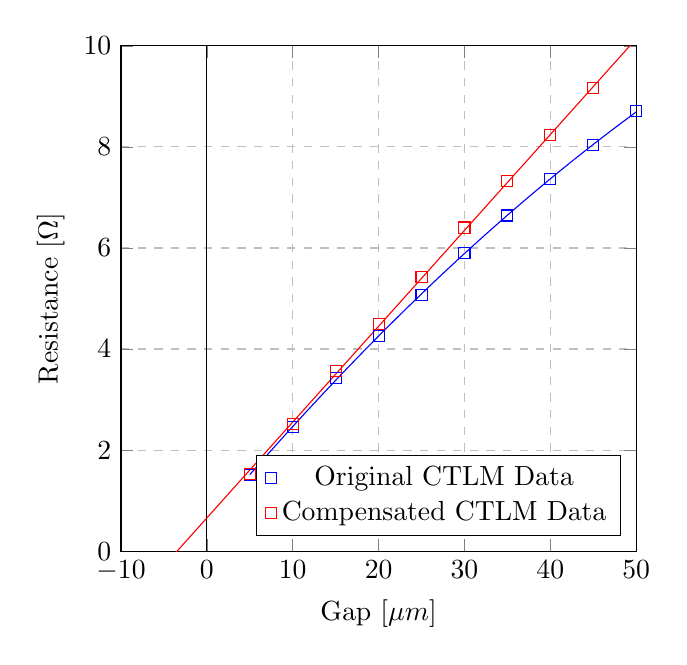
\begin{tikzpicture}

\begin{axis}[
    %title={Temperature dependence of CuSO$_4\cdot$5H$_2$O solubility},
    xlabel={Gap [$\mu m$]},
    ylabel={Resistance [$\Omega$]},
    height=8cm,
    width=0.67\textwidth,
    xmin=-10, xmax=50,
    ymin=0, ymax=10,
    xtick={-10, 0, 10, 20, 30, 40, 50},
    ytick={0, 2, 4, 6, 8, 10},
    % extra y ticks       = 0,
    % extra y tick labels = ,
    % extra y tick style  = { grid = major },
    legend pos=south east,
    ymajorgrids=true,
    xmajorgrids=true,
    grid style=dashed,
]

\addplot[color=blue, mark=square, only marks]
  coordinates {
  (5,1.505363832096823)
  (10,2.449740000726955)
  (15,3.421831099752043)
  (20,4.26394152103118)
  (25,5.070137988413258)
  (30,5.897088680026425)
  (35,6.64208850217324)
  (40,7.356653937259235)
  (45,8.039941315513527)
  (50,8.704528583743103)
};
  \addlegendentry{Original CTLM Data}

\addplot[color=red, mark=square, only marks]
    coordinates {
      (5,1.5245819322833463)
      (10,2.5136557475645573)
      (15,3.5587516564503536)
      (20,4.4966681982956205)
      (25,5.424233303346553)
      (30,6.403332285388977)
      (35,7.323979842935674)
      (40,8.242064238392762)
      (45,9.157502883492521)
      (50,10.085819749510799)
  };
    \addlegendentry{Compensated CTLM Data}

\addplot[color=black]
  coordinates{
    (0,0)
    (0,10)};


\addplot[color=blue,samples=100][domain=5:50]{-0.00077678*x^2 + 0.20218898*x + 0.5225879};

\addplot[color=red,samples=100][domain=-10:50]{0.18961899*x + 0.65853675};

\addplot[color=black] coordinates{(0,0) (10,0)};


\end{axis}
\end{tikzpicture}

\caption{Plot of resistance against CTLM gap size with the as measured data in blue and the data with the correction factor shown in \ref{eq:correction} applied shown in red. From the graph $2L_T = 3.473\mu m$, $2R_c = 0.659\Omega$, and $\rho_0 = $\hl{.......}}
\label{fig:ctlm_res}
\end{center}
\end{figure}


% \hl{6.25\%
%
% Plot CTLM results for one device from your group. Why do we use CTLMs over TLMs? Describe the salient features of the graph, and comment on any relationship to previous plots. Comment on why only the p-contact is analysed. [150 words max + Figures]}

Figures \ref{fig:ctlms_iv} shows the I-V plot for all gap size measurements from the circular transfer length method (CTLM). The CTLMs had a radius of $200\mu m$ and gap sizes from 5 to $50\mu m$ in steps of $5\mu m$. The plots for all gap sizes are close to linear implying that the contacts have an ohmic response.

The average resistance for each gap was found and plotted against the gap sizes, see figure \ref{fig:ctlm_res}. The true gap sizes were not measured and are assumed to be exactly as designed. Due to the nature of CTLMs, the radii of the two contacts cannot be equal. It is therefore necessary to include a correction factor which is found using equation \ref{eq:correction}

\begin{equation}
  C = \frac{1}{R_1}ln(\frac{R_1 + S}{R_1})
  \label{eq:correction}
\end{equation}

When the line of best fit for the corrected resistance values, shown in red, on figure \ref{fig:ctlm_res} are extrapolated it is found that the resistance values when the gap size is $0\mu m$ the resistance is $0.659\Omega$. This is equivalent to $2R_c$.



  \section{Commentary}
\label{sec:comment}

% \hl{15.625\%
%
% Highlight any process steps that you think may need more attention should you repeat the fabrication process.
% How would you redesign the process sequence if the scribe and break at process number 8 could be moved to the end? Comment upon how the LED operation varies with mesa diameter. Suggest how you may make the LED operate more efficiently. [300 words max + Figures].}

If the fabrication process were to be repeated in future, the etch time would be reduced since it etched $~67\%$ deeper than intended. The time would initially be halved then the depth measured before continuing the etching in 5 second periods. If the photomasks were to be redesigned at any point, careful consideration should be given to the alignment markers since they did not align.

If the scribe and break process was moved to the end, there it would be possible to us the CTLM to characterise a much larger number of LEDs with the same amount of measurements. Approximately $25\%$ of the current design is given over to testing whereas the same area could be used on a much larger wafer and drastically increase the yield.

The larger mesa diameters used by other students resulted in both more optically powerful LEDs and a larger current draw.


  \newpage

\pagestyle{empty}
\bibliographystyle{IEEEtran}
\bibliography{references.bib}


\end{document}
